
\documentclass[12pt,openany]{book}
%\usepackage{cclicenses}
\usepackage[letterpaper,  hmargin = { 1in},vmargin = { 1in}]{geometry}
\usepackage{hyperref}
\usepackage[T1]{fontenc}
\usepackage{multicol}
\newcommand{\mytitle}{Scivault Physics}
\usepackage{amsmath}
\usepackage{hyperref}
\usepackage{mathtools}
\usepackage{enumitem}
\usepackage{amssymb}
\usepackage{cleveref}
\usepackage{longtable}
\usepackage{appendix}
\usepackage{makeidx}
\usepackage[makeroom]{cancel}
\usepackage{siunitx}
\usepackage{gensymb}
\usepackage{tikz,bm}
\usepackage{float}
\usetikzlibrary{decorations.pathmorphing}
\usetikzlibrary{decorations.pathreplacing}
\usetikzlibrary{calc,angles,quotes}
\tikzset{
	samples=100,
}
\usetikzlibrary{arrows,shapes,positioning,shadows,arrows.meta}
\usetikzlibrary{decorations.markings}
\tikzstyle arrowstyle=[scale=1]
\tikzstyle directed=[postaction={decorate,decoration={markings,
		mark=at position .65 with {\arrow[arrowstyle]{stealth}}}}]
\tikzstyle reverse directed=[postaction={decorate,decoration={markings,
		mark=at position .65 with {\arrowreversed[arrowstyle]{stealth};}}}]
	
\usepackage[linewidth=1pt]{mdframed}
\setlength{\columnsep}{1cm}



\usepackage{pgfplots}
\pgfplotsset{compat=1.11}

% Variables
\pgfmathsetmacro\T{1}
\pgfmathsetmacro\A{0.2}
\pgfmathsetmacro\N{5}
\pgfmathsetmacro\D{\N*\T}

\makeindex

%%% To make index work,
% 1) Compile
%2) From base directory, run:
%   makeindex "Scivault Physics.idx"
%3) Compile again













\begin{document}
	\frontmatter
	\title{\mytitle}
	\author{Jonas Williamson}
	\date{Version \the\year\the\month\the\day}
	\maketitle

\normalsize
	\copyright \space \the\year\space by Jonas Williamson.  All Rights Reserved. 
	
		\vspace{2 in}	


	\vspace{1 in}

	\tableofcontents


\mainmatter


	
	
	
	
	
	

	
	


\chapter{Introduction}
\section{Dimensional Analysis and SI units}
\subsection{SI Units}
The \textbf{SI}\index{SI system of units} system of units is the standard used by many scientists throughout the world.  There are seven \textit{fundamental} or \textit{base} quantities from which all other measurements are derived.  These quantities are listed below:
 \index{Units, Fundamental}

\begin{center}

	
\begin{table}[ht]\caption{\textbf{SI Units}}% title of Table 
	\centering % used for centering table	
	\begin{tabular}{|c|c|c|}
		\hline \hline
		\textbf{Quantity} & \textbf{Unit} & \textbf{Unit Symbol}\\
		\hline
		time & second & s \\
		\hline
		length & meter & m \\
		\hline
		mass & kilogram & kg \\
		\hline
		electrical current & Ampere & A \\
		\hline
		temperature & Kelvin & K \\
		\hline
		amount of substance & mole & mol \\
		\hline
		luminous intensity & candela & cd \\
		\hline		
	\end{tabular}
	\label{table:nonlin}% is used to refer this table in the text
\end{table}
\end{center}

	Of these quantities, mass, time and length are quite common.  Thus, this system is sometimes called the MKS (meter, kilogram, second) system. In order to use any equations, all measurements must have correct units.  For example, if a time is expressed in hours, it must first be converted into seconds before any calculations can be attempted.  
	
	\subsection{Dimensional Analysis}
	Dimensional analysis \index{Dimensional Analysis} is the process in which the units associated with quantities create \textit{derived units}. \index{Units, Derived} For instance, when a distance is divided by a time, the units will be $ \frac{m}{s}$ (read \textit{meters per second}).  	
	
	Dimensional analysis is an important part of solving physics problems.  Often, correct dimensional analysis can help you determine if a problem has been solved correctly.  One should not even attempt to calculate an answer to a problem until the correct units have been verified. 

	\subsection{Unit Conversions} \index{Unit Conversions}
	Often you will find that you need to convert a measurement from one unit to another.  In order to do this, you must use a \textit{conversion factor.}  A conversion factor is a fraction that is based upon a statement of equality.  For instance, since 60 seconds = 1 minute, a conversion factor will look like either $\frac{60s}{1 min}$ or $\frac{1 min}{60s}$.  You should chose the version of the conversion factor that eliminates the units that you wish to convert.  
	
	
		\begin{mdframed}[backgroundcolor=blue!10!white]
		\begin{center}
			\textbf{Example \thesubsection}	\label{ex113}
		\end{center}
	
		\vspace{0.1in}	
		\textbf{Problem:} Convert 7.241 hours into seconds. 
		\vspace{0.1in}
		
		\textbf{Solution:} Begin by converting 7.241 hours into minutes.  Since 60 minutes = 1 hour, 
			\begin{equation*}
			7.241 \cancel{hr} \frac{60 min}{1 \cancel{hr}} = 434.46 min
			\end{equation*}
		
		Knowing that 1 minute = 60 seconds, we can use a second conversion factor to obtain seconds:
			\begin{equation*}
			434.46 \cancel{min} \frac{60 s}{1 \cancel{min}} = \boxed{26067.6s}
			\end{equation*}
		
		This problem could be solved in one step if you know that 1 hour = 3600 seconds. 
	
	\end{mdframed}


	
\begin{mdframed}[backgroundcolor=blue!10!white]
	\begin{center}
		\textbf{Example \thesubsection.2}	\label{ex1132}
	\end{center}
	
	\vspace{0.1in}	
	\textbf{Problem:} A car travels with a speed of 20 m/s.  What is this in miles per hour? 
	\vspace{0.1in}
	
	\textbf{Solution:} We begin by converting meters per second into meters per hour:
	\begin{equation*}
	20 \frac{m}{\cancel{s}} \cdot \frac{3600 \cancel{s}}{1 {hr}} = 72000 \frac{m}{hr}
	\end{equation*}
	
	We also need to know that 1 mile = 1609.34 meters:
	\begin{equation*}
		72000 \frac{\cancel{m}}{hr} \cdot \frac{1 mile}{1609.34 \cancel{m}} \approx 44.739 \frac{miles}{hr} 
	\end{equation*}
	
	
\end{mdframed}
		


\section{Vectors and Scalars}
In the study of physics, there are two types of quantities that we will deal with on a regular basis: \textit{scalars} and \textit{vectors}.  

A \textbf{scalar} is a quantity that you are already most likely very familiar with, as it is just a number; scalars have only a \textit{magnitude} (a number that represents how big or strong it is), and can sometimes include units.  Examples of scalars might be the number of people in a room, the mass of a car, or your age in years.  

\textbf{Vectors} are different from scalars because in addition to a magnitude, they contain a direction as well.  Examples of vectors might include 50 feet to the north, 5 m/s at a 33$^\circ$ angle, or 200 miles straight up.  
There are many ways of expressing vectors.  Symbollically, they are often written with an arrow over them.  For example, in the equation \color{blue} $\vec{F} = m \vec{a}$ \color{black}  both force and acceleration are vectors - meaning that both force and acceleration have a direction.  Sometimes vectors will be expressed in \textbf{bold} typeface.   Hence, the expression \\ \color{blue} \textbf{F} = m \textbf{a}  \color{black} is equivalent to the expression shown above.

The direction for vectors in 1 dimension is easy - all you need is a positive or a negative.  Usually, 1-dimensional motion takes place along the x-axis (left and right), but sometimes it will take place in the y- (forward and backward) and z- (up and down) dimensions.  For the purposes of this book, positive is to the right and up unless otherwise stated. 
In two dimensions, a vector requires two pieces of information.  One way of expressing a vector is in polar form.  Polar form in two dimensions includes a magnitude of the vector and an angle, usually measured from the x-axis.  There are several ways for writing this.  4 cm @ 15$^\circ$, \\ 4 cm $\angle 15^\circ$ and 4 cm at 15$^\circ$ North of East all represent the following displacement vector:



\begin{figure}[h]
	\caption{A vector represented graphically.} \label{figure:M1}
	\centering
	\begin{tikzpicture}
	
	\draw[thin,gray!40] (0,0) grid (4,2);
	\draw[<->] (0,0)--(4,0) node[right]{$x$};
	\draw[<->] (0,0)--(0,2) node[above]{$y$};
	\draw[line width=2pt,blue,-stealth](0,0)--(3.86,1.035) node[anchor=south west]{$\vec{d}$};
	
	
	
	
	\end{tikzpicture}
	
\end{figure}


	
	
	



	
	The magnitude of the above vector is 4 cm.  Mathematically, the magnitude of a vector can be written several ways, the most common being $\lvert \vec{A} \rvert$, though sometimes the magnitude of a vector can be written as the vector without the vector sign, as in $A$. 
	
	Unit vectors are vectors that have a length of one unit and are oriented along one axis.  The unit vector for the x-direction is written as $\hat{i}$ (pronounced i-hat).  $\hat{i}$ is a 1-unit long vector that is always parallel to the x-axis, and points in the direction of increasing x values.  Likewise, the y-direction and z-direction unit vectors are written as $\hat{j}$ and $\hat{k}$ respectively.  
	
	
	Because the surface of a paper is effectively 2-dimensional, it is very hard to draw lines that are oriented directly into or out of your paper. For this purpose, physicists have agreed to the following convention: vectors that point directly into your paper are notated by $\bigotimes$ .  Vectors that point directly out of your paper are shown by the symbol $\bigodot$.  
	
	Sometimes, vectors may be expressed in Cartesian coordinates.  This vector could either be expressed as an ordered pair (or triple) with square brackets, such as [3, 4, 5] cm, or as a linear combination of the unit vectors shown above, such as $5\hat{i} + 12 \hat{j} + 3 \hat{k}$  In each case, the distances in each direction are given by the numbers shown.  The vector in figure \ref{figure:M1} could be represented as: \color{blue} $\vec{d}  \approx 3.86 \hat{i} + 1.035 \hat{j}$.  \color{black}
	
	When converting between polar and cartesian forms for two dimensional vectors, a little trigonometry shows: 
		\begin{mdframed}[backgroundcolor=orange!20!white]
	
	\color{blue}
	\begin{multicols}{2}
		\begin{center}
			\begin{equation}
			x = r \cos(\theta)
			\label{eq11}
			\end{equation}
			
			\begin{equation}
			y = r \sin(\theta)
			\end{equation}

			\begin{equation}
			r = \sqrt{x^2+y^2}			
			\end{equation}

			\begin{equation}
			\theta=\tan^{-1}(\frac{y}{x})
			\label{eq14}
			\end{equation}		
		\end{center}
	\end{multicols}
	\color{black}
	\end{mdframed}
	
	In three dimensions, polar form comes in two types: \textbf{cylindrical} and \textbf{spherical}.  In cylindrical coordinates, expressed as [r, $\theta$, z],  the above conversions are used, and the z-coordinate remains unchanged from Cartesian form.  In spherical coordinates, the vector [r, $\theta$, $\phi$] includes a radial distance, an azimuthal angle and a polar angle. 

	
	
	
	
\section{Vector Mathematics}
	\subsection{Vector Addition} \index{Vectors, Addition}
	\subsubsection{Graphical Addition of Vectors} 
	When vectors are added graphically, they are added \textbf{head} to \textbf{tail}.  This means that the arrowhead for a first vector becomes the origin for the second vector.  The \textbf{resultant} vector is a straight line between the origin of the first vector and the head of the second.  
	
	
	\begin{mdframed}[backgroundcolor=blue!10!white]
		\begin{center}
			
			
			\textbf{Example \thesubsection}	\label{test}
		\end{center}
		
		\vspace{0.1in}
		\textbf{Problem:}  If $\vec{A} =  \hat{i} + 2 \hat{j} $ and $\vec{B} = 3 \hat{i} - \hat{j} $, 
		find $\vec{C}$ graphically given $\vec{C} = \vec{A} + \vec{B}$ 
		
		\vspace{0.1in}
		
		
		\textbf{Solution:} Begin by drawing $\vec{A}$:
		
		
			
		
		\begin{center}
			\begin{tikzpicture}
			\draw[thin,gray!40] (0,0) grid (4,2);
			\draw[<->] (0,0)--(4,0) node[right]{$x$};
			\draw[<->] (0,0)--(0,2) node[above]{$y$};
			\draw[line width=2pt,blue,-stealth](0,0)--(1,2) node[anchor=south east]{$\vec{A}$};

			\end{tikzpicture}
			
		\end{center}
	
		Now use the head of $\vec{A} $ as the origin for $\vec{B}$:
	
	
		\begin{center}
		
		
		
		
		
		
		\begin{tikzpicture}
		\draw[thin,gray!40] (0,0) grid (4,2);
		\draw[<->] (0,0)--(4,0) node[right]{$x$};
		\draw[<->] (0,0)--(0,2) node[above]{$y$};
		\draw[line width=2pt,blue,-stealth](0,0)--(1,2) node[anchor=south east]{$\vec{A}$};
		\draw[line width=2pt,red,-stealth](1,2)--(4,1) node[anchor=south west]{$\vec{B}$};

		\end{tikzpicture}		
		
	\end{center}
	
	The resulting vector is a straight line from the origin to the end of $\vec{B}$: 
	
	
	\begin{center}
		

		
		
		
		
			\begin{tikzpicture}
			\draw[thin,gray!40] (0,0) grid (4,2);
			\draw[<->] (0,0)--(4,0) node[right]{$x$};
			\draw[<->] (0,0)--(0,2) node[above]{$y$};
			\draw[line width=2pt,blue,-stealth](0,0)--(1,2) node[anchor=south east]{$\vec{A}$};
			\draw[line width=2pt,red,-stealth](1,2)--(4,1) node[anchor=south west]{$\vec{B}$};
			\draw[line width=2pt,green,-stealth](0,0)--(4,1) node[anchor=north west]{$\vec{C}$};
			\end{tikzpicture}
			
			
			
		\end{center}
		
		The resultant vector is given by $\boxed {\vec{C} = 4 \hat{i} + \hat{j}}$
		
	\end{mdframed}
	
	\subsubsection{Mathematical Addition of Vectors}
	Mathematical addition of vectors in Cartesian form is quite easy - simply add corresponding x- and y- values together.  For instance, in Example \ref{test} we are given  $\vec{A} =  \hat{i} + 2 \hat{j} $ and $\vec{B} = 3 \hat{i} - \hat{j} $.  Adding these together would give $\vec{C} = (1 +3) \hat{i} + (2-1)\hat{j} \longrightarrow \vec{C} =  4 \hat{i} + \hat{j} $.
	
	The easiest way to add vectors that are expressed in polar coordinates is to first convert them into cartesian coordinates using Equations \eqref{eq11} through \eqref{eq14} on page \pageref{eq11}.
	
	
	
	\subsection{The Dot Product} \index{Dot Product} \index{Vectors, Dot Product}
	\subsubsection{In Cartesian Form}
	When multiplying vectors, it is sometimes necessary to obtain a scalar result.  This is done through use of a dot product.  A dot product is written as $\vec{A} \cdot \vec{B} $.  This means to only multiply the components of the vectors that are in the same direction.  In cartesian coordinates, this can be done by multiplying corresponding components, then adding the products.  
	
		\begin{mdframed}[backgroundcolor=blue!10!white]
			\begin{center}
				\textbf{Example \thesubsection}	\label{example:dotproduct}
				
				
			\end{center}
		
		\textbf{Problem:} Given the vectors $ \vec{Y} = 2 \hat{i} + 3 \hat{j} $ and $\vec{Z} = -4 \hat{i} + 5 \hat{j}$ find the dot product of vectors Y and Z. 
		
		\vspace{.1in}
		
		\textbf{Solution:} Multiply coefficients from each vector, then add the products together:
		\begin{center}
			$2\times(-4) + 3\times 5 = -8 + 15 = \boxed{7}$ 
		\end{center}
		
		
		\end{mdframed}
	\subsubsection{In Polar Form}
	Often, vectors will be expressed in polar notation.  If this is the case, the dot product can be found my multiplying the magnitude of the first vector times the magnitude of the second vector times the cosine of the angle between:
	
	
	\begin{mdframed}[backgroundcolor=orange!20!white]
		\begin{equation}
			\label{equation:dotproduct}
		\vec{A} \cdot \vec{B} = \lvert \vec{A} \rvert  \lvert \vec{B} \rvert \cos{\theta}
		\end{equation}
		
	\end{mdframed}
	
	
	\vspace{0.1in}
	
	
		\begin{mdframed}[backgroundcolor=blue!10!white]
		\begin{center}
			\textbf{Example \thesubsection.2}	\label{example:dotproduct2}
			\vspace{0.1in}
			
			
		\end{center}
		
		\textbf{Problem:} Given the vectors $ \vec{D} = 3 \angle 30^{\circ} $ and $\vec{E} = 5 \angle 60^{\circ}$ find the dot product of vectors D and E. 
		
		\vspace{.1in}
		
		\textbf{Solution:}  We begin by graphing both vectors starting from a common origin:
		\begin{center}
		\begin{tikzpicture}
		\draw[thin,gray!40] (0,0) grid (3,5);
		\draw[<->] (0,0)--(3,0) node[right]{$x$};
		\draw[<->] (0,0)--(0,5) node[above]{$y$};
		\draw[line width=2pt,blue,-stealth](0,0)--(2.598,1.5) node[anchor=south east]{$\vec{A}$};
		\draw[line width=2pt,red,-stealth](0,0)--(2.5,4.33) node[anchor=south west]{$\vec{B}$};
		
		\end{tikzpicture}	
			

		\end{center}
			
			Noticing that the angle between the two vectors is $30^\circ$, we can use equation 1.5 to calculate:
			
			\begin{center}
				$ 		\vec{D} \cdot \vec{E} = \lvert \vec{D} \rvert  \lvert \vec{E} \rvert \cos{\theta} = (3)(5)\cos30^\circ \approx \boxed{12.990} $
			\end{center}
		
		
		
		
		\begin{center}
			
		\end{center}
		
		
	\end{mdframed}
	
	
	
	\subsection{The Cross Product}  \index{Cross Product} \index{Vectors, Cross Product}
	\subsubsection{Cross Products In Cartesian Form}
	Sometimes two vectors will be multiplied in such a way that they will result in another vector.  This is called a \textbf{Cross Product}.  A cross product is inherently a three-dimensional operation.  A cross product can be found by calculating the determinant of a matrix:  
	
\begin{mdframed}[backgroundcolor=orange!20!white]
\begin{equation}
 \vec{A} \times \vec{B} = 	\begin{vmatrix}
				\hat{i} & \hat{j} & \hat{k}\\
				A_x & A_y & A_z \\
				B_x & B_y & B_z 
				\end{vmatrix} 
				\label{equation:16}
\end{equation}
\end{mdframed}	

	
The most common way to find the determinant of the above matrix is by using minors:
\begin{center}
$
 \vec{A} \times \vec{B} = 	\begin{vmatrix}
	\hat{i} & \hat{j} & \hat{k}\\
	A_x & A_y & A_z \\
	B_x & B_y & B_z 
\end{vmatrix} 
= \hat{i} \begin{vmatrix}
	A_y & A_z \\
	B_y & B_z 
\end{vmatrix} - \hat{j} \begin{vmatrix}
A_x & A_z \\
B_x & B_z 
\end{vmatrix} + \hat{k} \begin{vmatrix}
A_x & A_y \\
B_x & B_y 
\end{vmatrix}
$
\end{center}

This finding the determinate of each of the 2x2 matrices yields:
\begin{center}
	$ \vec{A} \times \vec{B} = 	\hat{i} (A_y B_z - A_z B_y) - \hat{j}(A_x B_z - A_z B_x)+ \hat{k}(A_x B_y - A_y B_x)
$\end{center}



	\begin{mdframed}[backgroundcolor=blue!10!white]
	\begin{center}
		\textbf{Example \thesubsection}	\label{example:crossproductcartesian}
		\vspace{0.1in}
		
		
	\end{center}
	
	\textbf{Problem:} Given the vectors $ \vec{V} = 2 \hat{i} + 3 \hat{j} $ and $\vec{W} = -4 \hat{i} + 5 \hat{j}$ find the cross product of vectors V and W. 
	
	\vspace{.1in}
	
	\textbf{Solution:}  Begin by creating a matrix, as shown in equation \eqref{equation:16}.  Since both vectors lie in the X-Y plane, the Z-components for both vectors are zero:
	
	\begin{center}
		$\vec{V} \times \vec{W} =  \begin{vmatrix}
		\hat{i} & \hat{j} & \hat{k} \\
		2 & 3 & 0\\
		-4 & 5 & 0		
		\end{vmatrix}$

	\end{center}

Now, use expansion by minors to create three two-by-two matrices:

\begin{center}
	$\vec{V} \times \vec{W} =  \begin{vmatrix}
	\hat{i} & \hat{j} & \hat{k} \\
	2 & 3 & 0\\
	-4 & 5 & 0		
	\end{vmatrix} = \hat{i} \begin{vmatrix}
		3 & 0 \\
		5 & 0 
	\end{vmatrix} - \hat{j} \begin{vmatrix}
		2 & 0 \\
		-4 & 0 
	\end{vmatrix} + \hat{k} \begin{vmatrix}
		2 & 3 \\
		-4 & 5 
	\end{vmatrix}
	$
\end{center}

Finding the determinate of each of the two-by-two matricies yields: 
\begin{center}
	$	\vec{V} \times \vec{W} = \hat{i}(3\cdot0-0\cdot5)-\hat{j}(2\cdot0-0\cdot(-4))+\hat{k}(2\cdot5-3\cdot(-4))$
\end{center}

Both the x-component and the y-components of this cross product are zero.  Thus, 
\begin{center}
	$	\boxed{\vec{V} \times \vec{W} = 22 \hat{k}}$
\end{center}


\end{mdframed}
	
	There are some important things you may wish to note.  
	\begin{enumerate}
		\item The cross product is not commutative.  That is, $\vec{A} \times \vec{B} \neq \vec{B} \times \vec{A}$.  In fact, the two cross products are in exactly opposite directions.  
		\item The cross product of two vectors is always a vector that is perpendicular to both of the original vectors.  
	\end{enumerate}


\subsubsection{Cross Products In Polar Form}
	When vectors are expressed in polar form, a cross product can often be found using two steps.  To find the magnitude of the resulting vector, one would use the following equation:
	
\begin{mdframed}[backgroundcolor=orange!20!white]
	\begin{equation}
	\lvert \vec{A} \times \vec{B} \rvert = 	\lvert \vec{A} \rvert \lvert\vec{B} \rvert \sin \theta
	\label{Equation:17}
	\end{equation}
\end{mdframed}	

\label{RHR1}
In Equation \ref{Equation:17}, $\theta$ is the angle between the two vectors.  To find the direction of the resulting vector, use the \textbf{First Right Hand Rule}.  \index{Right Hand Rule, First} \index{First Right Hand Rule} To use this rule, you point your index finger in the direction of the first vector to be multiplied.  Your middle finger is then pointed in the direction of the second vector to be multiplied.  Your thumb will point in the direction of the resultant vector, as shown in the image: 

\begin{center}
	\begin{figure}[h]
		\centering
	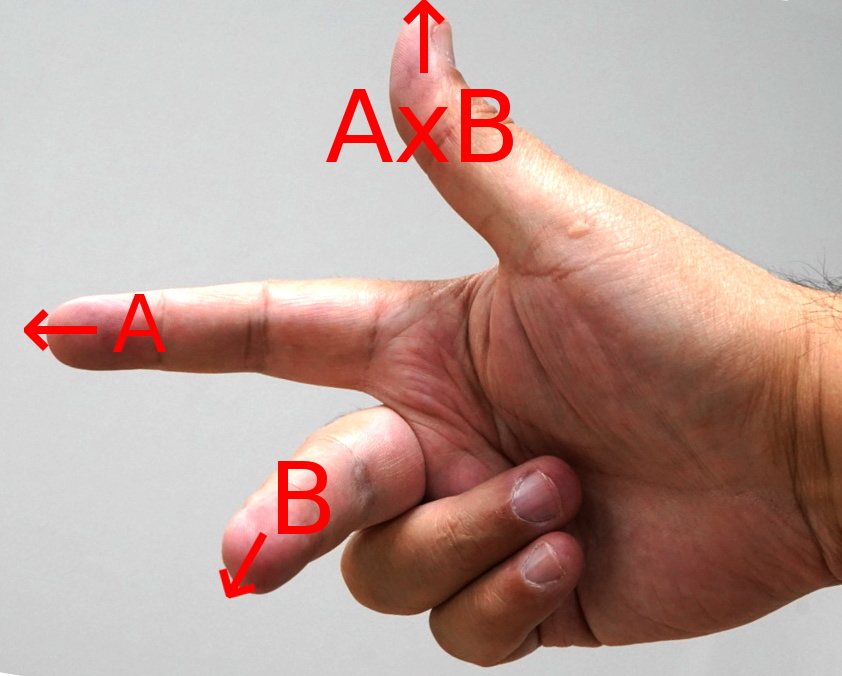
\includegraphics[height=2in]{./Chapters/Ch01-intro/righthandrule.JPG}	
	\caption{The First Right Hand Rule}
	\end{figure}
	
\end{center}

The right had rule is easiest to use when the first two vectors are at $90^\circ$ to each other.  However, even if the first two vectors are not at right angles to each other, the resultant vector of a cross product will always be perpendicular to the plane of the first two vectors.  


\newpage
\section{Exercises for Chapter 1}

\begin{multicols}{2}


	\begin{enumerate}


	\subsection*{Section 1.1: Dimensional Analysis}
		\item What are the units for each of the following?
			\begin{enumerate}
				\item $\frac{5 m}{2 s}$
				\item $\frac{10kg}{5s}$
				\item $\frac{140 kg \cdot 15 m}{23 s} $
				\item $\frac{(\frac{15m}{15s})}{14 s} $
				
			\end{enumerate}
	\subsection*{Section 1.2: Vectors and Scalars}
		\item Given the vector $4\hat{i} - 3 \hat{j}$, represent the vector (a) graphically and (b) in polar form.  
		\item George walks 200 meters north, then walks 400 meters north.  What is the vector from his starting position to his ending position in (a) cartesian form and (b) polar form (take north as 0 degrees).  
	\subsection*{Section 1.3: Vector Mathematics}
		\item Addition - cartesian
		\item Addition - polar
		\item Dot Product - Cartesian
		\item Dot Product - polar
		\item Cross Product - cartesian
		\item Cross Product - polar
		
		
	\end{enumerate}	
\end{multicols}	
	




\chapter{Kinematics in One Dimension}
\section{Distance and Displacement} \index{Distance}

You are probably already familiar with the concept of \textbf{distance} - you might get in your car and drive a total of 1.2 miles to school, turning right after 0.45 miles, according to your car's odometer.  Distance is a scalar that tells you how far something traveled.  The symbol d usually represents distance.

While you may have traveled a total distance of 1.2 miles from your school, you are significantly less than 1.2 miles away from home; in fact, you are approximately 0.874 miles from home, following a direct path directly from your home to the school, at an angle of $59^\circ $(not worrying that this path might take you through someone's back yard or kitchen).


  \textbf{Displacement} \index{Displacement} is a vector that tell you how far something is from the origin, and is independent of the path taken to get there.  The displacement vector is commonly symbolized by $\vec{r}$ though sometimes it may be written as $\vec{d}$ or $\vec{x}$. 

\section{Average and Instantaneous Speed and Velocity}

\textbf{Speed} is a scalar value that represents the change in distance per change in time of an object.  Speed is usually represented with the symbol $v$, without the vector sign.  You are probably already familiar with this quantity, since the speedometer on your family car measures speed.  For the purposes of physics, speed has little value because it is a scalar that tells us nothing of direction.  Much more useful is the concept called velocity.  Velocity and speed are related much like distance and displacement.  

\textbf{Velocity} is the change in displacement of an object per unit time, and as such is a vector.  Positive velocities indicate that the object is moving forward, relative to the axis in question, and negative velocities generally mean that the object is moving backward, relative the the axis.  The average velocity of an object is given by:
\begin{mdframed}[backgroundcolor=orange!20!white]
	\begin{equation}
	\overrightarrow{v_{avg}} = \frac{\Delta\vec{r}}{\Delta t} 
		\label{eqn:velocity}
	\end{equation}
\end{mdframed}

Average velocity is useful if an object's velocity is not changing.  However, many times it is more useful to talk about instantaneous velocity.  Instantaneous velocity tells us how fast an object is moving at a given instant in time.  In order to calculate instantaneous velocity, we must allow our time interval in the above formula to become infinitesimally small.  In this case, a little calculus proves:
\begin{mdframed}[backgroundcolor=orange!20!white]
	\begin{equation}
	\vec{v} = \frac{d\vec{r}}{dt}
	\label{equation:instantaneousvelocity}
	\end{equation}
\end{mdframed}	
	
	Calculation of average velocity is rather straightforward, assuming you know both distance traveled and the time it took.  If an object is not speeding up or slowing down during a specific time interval, the instantaneous velocity at any time during this interval is equal to the average velocity.  If the object does speed up or slow down during the time interval in question, the average velocity and the instantaneous velocity at a certain time during the interval are not necessarily the same. 
	
\begin{mdframed}[backgroundcolor=blue!10!white]
		\begin{center}


		\textbf{Example \thesection.1}	
	\end{center}

\textbf{Problem: }You ride your bicycle in a straight line for a distance of 73 meters in 12.5 second.  What is your average speed?
\vspace{0.1in}

\textbf{Solution:} 
Begin by drawing a diagram:


\begin{equation*}
 v_{avg}  = \frac{d}{t} = \frac{73m \hspace{0.05in} \hat{i}}{12.5s}  = 5.84 \frac{m}{s} \hspace{0.05in} \hat{i}
\end{equation*}

\end{mdframed}
	\vspace{0.1in}
	
\begin{mdframed}[backgroundcolor=blue!10!white]
	\begin{center}
		
		
		\textbf{Example \thesection.2}	
	\end{center}
	
	\textbf{Problem: }A bicyclist rides his bike to the east.  His position (in meters) is given by the following expression:
	\begin{equation*}
	\vec{r} = (0.5 t^2 + 4t) \hat{i}
	\end{equation*}
	\begin{enumerate}[label=\alph*.]
		\item What is his average velocity from t = 0 to t = 5 seconds?
		\item What is his instantaneous velocity at t=3 seconds?
	\end{enumerate}
	\vspace{0.1in}
	\textbf{Solution:} \begin{enumerate}[label=\alph*.]
		\item The total displacement (in meters) after five seconds is given by: 
		\begin{equation*}
		\hat{r} = (0.5 \times (5s)^2+4\times 5s) \hspace{0.05in} m \hspace{0.05in} \hat{i} = 32.5 \hspace{0.05in} m \hspace{0.05in} \hspace{0.05in} \hat{i}
		\end{equation*}
		Thus, the average velocity is - 
	\begin{equation*}
	\overrightarrow{v_{avg}}  = \frac{\vec{d}}{t} = \frac{32.5 m \hspace{0.05in} \hat{i}}{5s}  = \boxed{6.5 \frac{m}{s} \hspace{0.05in} \hat{i}}
	\end{equation*}
	
	
	
	\item The instantaneous velocity of an object is found using a derivative with respect to time.  Thus,
	
	\begin{equation*}
	\vec{v} = \frac{d\vec{r}}{dt} = \frac{d}{dt} (0.5 t^2 + 4t) \hat{i} = (t + 4) \hat{i} 
	\end{equation*}
	
	Evaluating this at t=3s yields:
	
	\begin{equation*}
	\vec{v} = (3 + 4) \hat{i} = 7 \frac{m}{s} \hat{i}
	\end{equation*}
	\end{enumerate}
	
\end{mdframed}

	
	
	
	

\section{Relative Motion at Constant Velocity}


\section{Acceleration}
\subsection{Average Acceleration} \index{Acceleration, Average}
Velocity is not always constant.  For instance, when you are driving through a city, there are times when you might be going 30 mph, and there are times when you might be stopped at a streetlight.  City driving requires you to speed up at some times, and slow down at other times – your velocity changes as a function of time.  Change in velocity per change in time is called acceleration.  
Keep in mind, both speeding up and slowing down are forms of acceleration.  In the case that an object is traveling with a positive velocity, slowing down causes negative acceleration (or deceleration).
Like velocity, acceleration comes in two basic types – average and instantaneous.  To find average velocity, we calculate the change in velocity per change in time:

\begin{mdframed}[backgroundcolor=orange!20!white]
	\begin{equation}
	\overrightarrow{a_{avg}} = \frac{\Delta \vec{v}}{\Delta t} 
	\label{equation:averageacceleration}
	\end{equation}
\end{mdframed}	
Keep in mind that this can be expressed as:
\begin{mdframed}[backgroundcolor=orange!20!white]
	\begin{equation}
	\overrightarrow{a_{avg}} = \frac{\overrightarrow{v_f} - \overrightarrow {v_i}}{\Delta t}
	\label{equation:averageaccelerationalt}
	\end{equation}
\end{mdframed}	


where $v_f$ and $v_i$ are final velocity and initial velocity, respectively.  Sometimes final velocity is expressed as $v$ and initial velocity is symbolized as $v_0$. 

\subsection{Instantaneous Acceleration} \index{Acceleration, Instantaneous}

Instantaneous velocity is found by letting the time interval in question become infinitesimally small.  A little calculus proves that:
\begin{mdframed}[backgroundcolor=orange!20!white]
	\begin{equation}
	\vec{a} = \frac{d \vec{v}}{dt} 
	\end{equation}
\end{mdframed}

Combining this with equation \ref{equation:instantaneousvelocity}, we find:
\begin{mdframed}[backgroundcolor=orange!20!white]
	\begin{equation}
	\vec{a} = \frac{d^2 \vec{r}}{dt^2} 
	\end{equation}
\end{mdframed}


\begin{mdframed}[backgroundcolor=blue!10!white]
	\begin{center}
		
		
		\textbf{Example \thesection}	
	\end{center}
	\vspace{0.1in}
	
	\textbf{Problem: } A car is traveling 20 m/s in the positive x direction.  The driver sees a red light, and applies the brakes, causing the vehicle to come to a stop in 4 seconds.  What is the average acceleration caused by the brakes?
	
	\vspace{0.1in}
	
	\textbf{Solution:} Using the definition of Average Acceleration from Equation \ref{equation:averageaccelerationalt}, we find:
	
	\begin{equation*}
			\overrightarrow{a_{avg}} = \frac{\overrightarrow{v_f} - \overrightarrow {v_i}}{\Delta t} = \frac{0 \frac{m}{s} \hat{i} - 20 \frac{m}{s} \hat{i}}{4 s}   = -5 \frac{m}{s^2} \hat{i}
	\end{equation*}
\end{mdframed}

\section{The Kinematic Equations} 
\subsection{The Kinematic Variables} \index{Kinematic Variables}
There are five variables that are often used to solve problems involving constant acceleration.  These variables are listed below:

\begin{center}
	
	
	\begin{table}[ht]\caption{\textbf{The Kinematic Variable}}% title of Table 
		\centering % used for centering table	
		\begin{tabular}{|c|c|c|}
			\hline \hline
			\textbf{Quantity} & \textbf{Variable} & \textbf{Units} \\
			\hline
			Displacement & $\vec{d}$ or $\vec{x}-\vec{x_0}$  & m \\
			\hline
			
			Initial Velocity & $\vec{v_i}$ or $\vec{v_0}$  & m/s \\
			\hline
			
			Final Velocity & $\vec{v_f}$ or $\vec{v}$  & m/s \\
			\hline
			
			Acceleration & $\vec{a}$   & $m/s^2$ \\
			\hline
			
			time & $t $  & s \\
			\hline
		\end{tabular}
		\label{table:kinematic1d}% is used to refer this table in the text
	\end{table}
\end{center}

\subsection{The Kinematic Equations}

\index{Kinematic Equations} \label{kinematicequations}
Using the definitions above, and a little calculus (or a lot of algebra) we can prove the following four equations:
\begin{mdframed}[backgroundcolor=orange!20!white]
	\begin{center}
		\textbf{The Kinematic Equations}
	\end{center}
	\begin{multicols}{2}
		\begin{equation}
		\vec{d} = \frac{\overrightarrow{v_f} + \overrightarrow{v_i}}{2}  t
		\label{equation:kinematic1}
		\end{equation}
			
		\begin{equation}
		\overrightarrow{v_f} = \overrightarrow{v_i} + \vec{a} t
		\label{equation:kinematic2}
		\end{equation}	
			
		\begin{equation}
		\vec{d} = \overrightarrow{v_i} t + \frac{1}{2}\vec{a}{t}^2
		\label{equation:kinematic3}
		\end{equation}
		
		\begin{equation}
		\overrightarrow{v_f}^2 = \overrightarrow{v_i}^2 + 2\vec{a}\vec{d}
		\label{equation:kinematic4}
		\end{equation}
		
		
			
		\end{multicols}
	\end{mdframed}

These equations enable you to solve the vast majority of kinematic problems.  Keep in mind that these equations should only be applied in one direction at at time – meaning that 2-dimensional and 3-dimensional problems will require you to split all the quantities into component vectors before you can solve these equations in each direction separately. It should also be noted that these equations assume constant acceleration.  If the acceleration of the object is changing, the equations are not valid.



\section{Vertical Motion and Gravity}

One of the most common types of acceleration we experience every day is the acceleration due to gravity.  Acceleration due to gravity is given a special symbol: g.  On Earth, $g \approx  9.81 \frac{m}{s^2}$.  Keep in mind that this value is only useful for calculations involving gravity that take place on the Earth's surface.  All planets, stars, and celestial bodies (in fact, all objects with any mass) have their own gravitational acceleration.  Acceleration due to gravity on the moon, for instance, is $1.62 \frac{m}{s^2}$.    

Objects undergo free fall when they are allowed to continue to accelerate due to gravity until they impact something that breaks their fall (often this is the ground).  In order to make the calculations easier, we often ignore air resistance.

Because gravity at the Earth's surface is downward, sign conventions become a little more important than previously.  If upward is positive, g will have a negative sign attached to it to indicate the direction of acceleration.  


\begin{mdframed}[backgroundcolor=blue!10!white]
	\begin{center}
		
		
		\textbf{Example \thesection}	
	\end{center}
	\vspace{0.1in}
	
	\textbf{Problem: } You are standing on top of a building.  You drop a rock  from the top of the building, and let it free fall until it hits the ground, 3.2 seconds later.  
	\begin{enumerate}[label=\alph*.]
		\item What is the height of the building?
		\item An identical building is build on the moon.  How long does it take the rock to fall in this case?
	\end{enumerate}

	\textbf{Solution:}
	\begin{enumerate}[label=\alph*.]
		\item To solve for distance, we apply equation 1.5.3 in the y-direction, and substitute ay = g and vi = 0 m/s,:
		
		\item Because we know that vi = 0 m/s, and ay = gm = 1.62 m/s2, we can let the final term drop out of equation 1.5.3 to yield:
	\end{enumerate}
\end{mdframed}





\chapter{Graphing Motion}
	\section{Position vs Time Graphs}
		\subsection{Constant Position}
		\subsection{Constant Velocity}
		\subsection{Constant Acceleration}
	\section{Velocity vs Time Graphs}
		\subsection{Constant Position}
		\subsection{Constant Velocity}
		\subsection{Constant Acceleration}
	\section{Acceleration vs Time Graphs}
		\subsection{Constant Position}
		\subsection{Constant Velocity}
		\subsection{Constant Acceleration}	
	

	



\chapter{Kinematics in Two Dimensions}
	\section{Introduction}
	
	When an object is moving in two (or three) dimensions at once - like when it moves both horizontally and vertically at the same time - the motion of the object in each dimension is completely independent.  This means that each dimension will have its own set of kinematic variables.  The only kinematic variable that can be used in all directions is time, since time is a scalar and does not have a direction.  Thus, instead of only five kinematic variables, problems will have sets of five variables in each direction, with time counting for every dimension.  
	
	
{\renewcommand{\arraystretch}{1.2}
\begin{center}
	
	
	\begin{table}[ht]\caption{\textbf{Kinematic Variables in Multiple Dimensions}}% title of Table 
		\centering % used for centering table	
		\begin{tabular}{|c|c||c|c|}
			\hline \hline
			\textbf{Quantity} & \textbf{Variable} & \textbf{Quantity} & \textbf{Variable}  \\
			\hline
			Horizontal Displacement & $\vec{d_x}$ or $\vec{x}-\vec{x_0}$  & Vertical Displacement & $\vec{d_y}$ or $\vec{y}-\vec{y_0}$ \\
			\hline
		
			Horizontal Initial Velocity & $\vec{v_{ix}}$ or $\vec{v_{0x}}$  & Vertical Initial Velocity & $\vec{v_{iy}}$ or $\vec{v_{0y}}$ \\
\hline

			Horizontal Final Velocity & $\vec{v_{fx}}$ or $\vec{v_x}$  & Vertical Final Velocity & $ \vec{v_{fy}}$ or $\vec{v_y}$ \\ 
	\hline
	Horizontal Acceleration & $\vec{a_x}$  &  Vertical Acceleration & $\vec{a_y} $ \\
	\hline
	\multicolumn{2}{|c|}{Time} & \multicolumn{2}{|c|}{$t$} \\
	\hline
		
		\end{tabular}
		\label{table:kinematic2d}% is used to refer this table in the text
	\end{table}
\end{center}

\section{Projectiles}
\index{Projectiles}

A \textbf{projectile} is any object that meets the following critera:
\begin{itemize}
	\item The object is in \textit{free-fall}.  That is, Gravity is the only force that acts on the object (all other forces are negligable).
	\item The object is moving in two dimensions at the same time.  Most often, describe it as moving both horizontally and vertically at the same time.  
\end{itemize}


\subsection{Horizontally Launched Projectiles}
	\index{Projectiles, Launched Horizontally}
Often, projectiles will be launched horizontally, such as when a ball rolls off a table, or when an archer shoots a perfectly level arrow.  In this case, the math is somewhat easier to deal with.  The initial velocity stated in the problem will be entirely horizontal, and the initial vertical velocity will be zero.


\begin{mdframed}[backgroundcolor=blue!10!white]
	\begin{center}
		
		
		\textbf{Example \thesection.1}	
	\end{center}
	
	\textbf{Problem: } A ball is rolling 2.1 m/s when it rolls off the edge of a 1.3 meter high table.
	\begin{enumerate}
		\item How long is the ball in the air?
		\item How far, horizontally, does the ball land from the edge of the table?
		\item What is the magnitude of the final velocity of the ball?
		\item What is the angle of impact?
	\end{enumerate}
	\vspace{0.1in}
	
	\textbf{Solution:} 
	Begin by drawing a diagram:
	
	\begin{tikzpicture}
		% Draw the table
		%\draw[thick] (0,0) rectangle (1,-1.3);
		%\node at (0.5, -1.4) [below] {Table (1.3 m)};
		
		% Draw the ball's initial position
		\filldraw[black] (0.5,0) circle (0.1);
		%\node at (0.4, 0) [left] {Ball};
		
		% Draw the trajectory of the ball
		\draw[->, thick, dashed] (0.5,0) .. controls (3.5,-1) and (5,-2.5) .. (6,-3.3);
		
		 Draw initial velocity components
		\draw[->, thick, red] (0.5,0) -- (2,0);
		\node at (1.25,0) [above,red] {$v_{0} = 2.1\, \text{m/s}$};
		
		% Draw initial downward velocity
		%\draw[->, thick, blue] (0.5,0) -- (0.5,-0.8);
		%\node at (0.5,-0.4) [left] {$v_y = 0\, \text{m/s}$};
		
		% Draw horizontal and vertical distance markers
		\draw[|-|] (6,0) -- (6,-3.3);
		\node at (6.6,-1.65) [right] {$y-y_0 = \SI{1.3} {m}$};
		
		\draw[|-|] (0.5,-3.3) -- (6,-3.3);
		\node at (3.25,-3.6) [below] {$x-x_0$};
		
		%Draw the coordinate system
			\draw[->,blue] (-1.5,1) -- (-1.5,0.5);
		\node at (-1.5,0.4) [below,blue] {+y};
		
			\draw[->,blue] (-1.5,1) -- (-1,1);
			\node at (-0.9,1) [right,blue] {+x};

		
		% Final velocity and angle markers
		%\draw[->, thick, green] (6,-3.3) -- (6.5,-4);
		%\node at (6.5,-3.6) [right] {$\vec{v}$};
		
		%\draw[->] (6,-3.3) -- (7,-3.3);
		%\node at (7,-3.3) [above] {$v_x$};
		
		%\draw[->] (6,-3.3) -- (6,-4.5);
		%\node at (6,-4.5) [left] {$v_y$};
		
		% Draw angle of impact
		%\draw (6,-3.3) arc[start angle=-90, end angle=-60, radius=1];
		%\node at (6.8,-3.8) {$\theta$};
		
	\end{tikzpicture}
	
	You may notice from the coordinate system that the downward direction has been chosen as +y.  This will help us to avoid needing negatives in the problem.
	
	Next, we create a table with each of the kinematic variables for each dimension:
	
	\begin{longtable}{|c l | c l|}
		\hline
		\multicolumn{2}{|c|}{\textbf{Horizontal}} & \multicolumn{2}{|c|}{\textbf{ Vertical}} \\
		\hline
		$\vec{x}-\vec{x_0}$ =&     & $\vec{y}-\vec{y_0} = $ & $\SI{1.3}{m}$ \\
		\hline
		$\vec{v_{0x}} = $ & $\SI{2.1}{m/s}$ & $\vec{v_{0y}} = $ & $\SI{0}{m/s}$ \\
		\hline
		$v_x = $&  & $v_y = $ &  \\
		\hline
		$a_x = $ & $\SI{0}{m/s^2}$ & $a_y = $ & $\SI{9.81}{m/s^2}$ \\ 
		\hline
		\multicolumn{2}{|r}{$t = $} & \multicolumn{2}{l|}{  }  \\
		\hline
	\end{longtable}
	
	\begin{enumerate}
		\item We see that the vertical direction has three variables, and can be used to calculate the time the ball is in the air, using equation \cref{equation:kinematic3}, applied in the vertical direction: 
		\begin{equation*}
			y - y_0 = \cancelto{0}{v_{0y}t} + \frac{1}{2}a_yt^2
		\end{equation*}

	Solving for t yields:
		\begin{equation*}
		t = \sqrt{\frac{2(y-y_0)}{a_y}} = \sqrt{\frac{2(\SI{1.3}{m})}{\SI{9.81}{m/s^2}}} \approx \SI{0.515}{s}
	\end{equation*}

	\item To find the distance the ball has traveled horizontally, we can use the same kinematic equation as the previous step, only this time, applied in the horizontal direction:
	\begin{equation*}
	x - x_0 = v_{0x}t + \cancelto{0}{\frac{1}{2}a_xt^2}
\end{equation*}

	\begin{equation*}
	x - x_0 = (\SI{2.1}{m/s})(\SI{0.515}{s})  \approx \SI{1.081}{m}
\end{equation*}
\item Finding the final velocity of the ball requires finding both the x- and y- components of the final velocity:
	\begin{equation*}
	v_x = v_{0x} + \cancelto{0}{a_x t} = \SI{2.1}{m/s}
\end{equation*}

	\begin{equation*}
	v_y = \cancelto{0}{v_{0y}} + a_y t = \SI{9.81}{m/s^2} \SI{0.515}{s} \approx \SI{5.050}{m/s}
\end{equation*}
	
	
	We can use these components of the final velocity to determine v according to the following diagram:
	
	\begin{tikzpicture}
		% Draw the vertical side (v_x)
		\draw[->, thick] (0,0) -- (0,-3) node[midway, left] {$v_y = \SI{5.050}{m/s}$};
		
		% Draw the horizontal side (v_y)
		\draw[->, thick] (0,-3) -- (2,-3) node[midway, below] {$v_x = \SI{2.1}{m/s}$};
		
		% Draw the hypotenuse (v)
		\draw[->, thick] (0,0) -- (2,-3) node[midway, above right] {$v$};
		
		\node at (1.8,-3) [above left,blue] {$\theta$};
		
	\end{tikzpicture}

		Using the pythagorean theorum, we find:
			\begin{equation*}
			v = \sqrt{v_x^2 + v_y^2} = \sqrt{(\SI{2.1}{m/s})^2+(\SI{5.050}{m/s})^2} \approx \SI{5.470}{m/s}
		\end{equation*}
	
	\item The angle of impact is marked as \color{blue} $\theta$ \color{black} in the diagram for part 3.  We can find the angle of impact by using trigonometry.  Using tangent yields:
	
			\begin{equation*}
	\tan {\theta} = \frac{opp}{adj} 
	\end{equation*}

	\begin{equation*}
	\theta = \tan^{-1} (\frac{opp}{adj}) = \tan^{-1} (\frac{v_y}{v_x}) = \tan^{-1} (\frac{\SI{5.050}{m/s}}{\SI{2.1}{m/s}}) \approx 67.420 \degree
	\end{equation*}

		
	\end{enumerate}

	
\end{mdframed}	
	
	
	
	
	
	\subsection{Projectiles Launched at an Arbitrary Angle}
	\index{Projectiles, Launched at an Arbitrary Angle}
	\subsubsection{Projectiles Launched at an Arbitrary Angle on Level Ground}
	\subsubsection{Projectiles Launched at an Arbitrary Angle on Uneven Ground}
	\subsubsection{Projectiles Launched at an Arbitrary Angle Near a Mountain or Hill}
		
		


	



\chapter{Newtons Laws}
	\section{Newton's First Law}
	\section{Newton's Second Law}
	\section{Newton's Thrid Law}
	\section{Applications of Newton's Laws}
		\subsection{Friction}
		\subsection{Elevators}
		\subsection{Pulleys}
		


	


	
\chapter{Work and Energy}

	
	\section{Energy}
	\index{Energy}
	\gls{energy} is the ability of an object or system to create a change.  In the SI system, the unit for energy is $\frac{kg m^2}{s ^2}$, which is given the name \gls{joule}s (J).  
	
	Though energy can be found in many forms, there are three basic categories of energy: mechanical energy, chemical energy, and Electromagnetic Energy (Light).  This chapter focuses on the forms of \gls{mechanicalenergy} , which is the sum of kinetic energy and potential energy.  
	
	
	
	
	\subsection{Kinetic Energy} \index{Kinetic Energy} \label{Kinetic Energy} \index{Energy, Kinetic}
	\gls{kineticenergy} is energy of motion.  Any object that is moving has kinetic energy.  Kinetic energy cannot be negative.  The formula for kinetic energy is: 
		\begin{mdframed}[backgroundcolor=orange!20!white]
		\begin{equation}
		K = \frac{1}{2}mv^2 
		\label{eqn:kineticenergy}
		\end{equation}
	\end{mdframed}
	
	
	
	\begin{mdframed}[backgroundcolor=blue!10!white]
		\begin{center}
			
			
			\textbf{Example \thesection.1}	
		\end{center}
		
		\textbf{Problem: } A 1000 kg car is traveling at 15 m/s.  What is its kinetic energy?
		\vspace{0.1in}
		
		\textbf{Solution:} 
		Begin by drawing a diagram:
		\vspace{0.1in}
		\begin{center}
			

		\begin{tikzpicture}
			
			% Draw the car
			\draw[fill=blue!30] (0,0) rectangle (2,1); % Car body
			\draw[fill=gray] (0.3,0) circle (0.2); % Rear wheel
			\draw[fill=gray] (1.7,0) circle (0.2); % Front wheel
			\node at (1, 1.2) {1000 kg}; % Car mass label
			
			% Draw the speed arrow
			\draw[->, thick, red] (2,0.5) -- (4,0.5) node[midway, above] {15 m/s};
			
		\draw[->, thick, blue] (-3,2) -- (-2.5,2);
				\node at (-2.5, 2)[blue, right] {+x}; % Car mass label
			
		\end{tikzpicture}
		\end{center}
	
	Since we know both the mass and the speed of the object, we can use equation \eqref{eqn:kineticenergy} to solve the problem:
	
		\begin{equation*}
		K = \frac{1}{2}mv^2 = \frac{1}{2}(\SI{1000}{kg})(\SI{15}{m/s})^2 = \SI{225000}{J}
	\end{equation*}

	
			
	
		
	\end{mdframed}
	
	\subsection{Potential energy} \index{Potential Energy} \index{Energy, Potential}
	\gls{potentialenergy} is energy that is stored.  Though there are many forms of potential energy, we will concentrate on two forms of stored energy in this section: gravitational potential energy and elastic potential energy.  In this text, potential energy is symbolized by the variable $U$, though it is quite common to find potential energy symbolized by the letters $PE$ as well. 
	
	A common misconception is that kinetic energy and potential energy cannot exist at the same time.  This is not the case, and object often have both kinetic energy and potential energy simultaneously.

	\subsubsection{Gravitational Potential Energy} \index{Gravitational Potential Energy} \index{Potential Energy, Gravitational} \index{Energy, Gravitational Potential}
	\gls{gravitationalpotentialenergy} is energy that is stored due to the interaction of an object with gravitational field.  When a relatively small object is in a uniform gravitational field (such as near the surface of a planet), the gravitational potential energy is given by: 
			\begin{mdframed}[backgroundcolor=orange!20!white]
		\begin{equation}
		U_g = mgh
		\label{eqn:gravitationalpotentialenergy}
		\end{equation}
	\end{mdframed}
	
	
 	\begin{mdframed}[backgroundcolor=blue!10!white]
 	\begin{center}
 		
 		
 		\textbf{Example \thesection.1}	
 	\end{center}
 	
 	\textbf{Problem: } A 2 kg block is held 3 meters above the ground. What is the gravitational potential energy of the block?
 	\vspace{0.1in}
 	
 	\textbf{Solution:} 
 	Begin by drawing a diagram:
 	\vspace{0.1in}
 	\begin{center}
 		\begin{tikzpicture}
 			
 			% Draw the ground line
 			\draw[thick] (-1,0) -- (3,0); % Ground line
 			\node at (-2,0) {Ground};
 			
 			% Draw the block positioned above the ground
 			\draw[fill=blue!30] (1,3) rectangle (2,4); % Block as a rectangle
 			\node at (1.5,3.5) {2 kg}; % Label for block
 			
 			% Draw the height indicator
% 			\draw[dashed] (2,3) -- (2,0); % Dashed line to indicate height
 			\draw[<->] (2.5,0.05) -- (2.5,3) node[midway, right] {3 m}; % Height label
 			
 			% Draw the gravitational force arrow
 %			\draw[->, thick, red] (1.5,3) -- (1.5,1.5) node[midway, left] {$F_g = mg$}; % Gravity force arrow
 			\draw[->, thick, blue] (-3,3) -- (-3,4);
 			\node at (-3,4.2) {+y};
 		\end{tikzpicture}
 		
 		We can now calculate potential energy using equation \eqref{eqn:gravitationalpotentialenergy}:
 		
 		\begin{equation*}
 			U_g = mgh = (\SI{2}{kg})(\SI{9.81}{\frac{m}{s^2}})(\SI{3}{m}) = \SI{58.86}{J} 
 		\end{equation*}
 		
 	\end{center}
 	
\end{mdframed}
 	
	
	
	
	\subsubsection{Elastic Potential Energy} \index{Elastic Potential Energy} \index{Potential Energy, Elastic}
	
	\index{Potential Energy, Gravitational}
	Springs and other stretchable materials that return to their original shape when not subjected to external forces store \gls{elasticpotentialenergy}.  For an ideal spring, the force the spring exerts is proportional to the distance it has been stretched.  This is called \gls{hookeslaw}: 
	
		\begin{mdframed}[backgroundcolor=orange!20!white]
		\begin{equation}
		\overrightarrow{F_s} = -k\vec{x}
		\label{eqn:hookeslaw}
		\end{equation}
	\end{mdframed}
	where $k$ is the \gls{springconstant}, \index{Spring Constant}  and $x$ is the distance the spring has been stretched or compressed from its equilibrium position.
	
	Some calculus can show that the energy stored in a spring that obeys Hooke's Law is: 
	
	\begin{mdframed}[backgroundcolor=orange!20!white]
		\begin{equation}
		U_s = \frac{1}{2}kx^2
		\label{eqn:elasticpotentialenergy}
		\end{equation}
	\end{mdframed}

	While all real springs convert mechanical energy into heat when stretching or compressing, the amount of energy lost as heat (a process called hysteresis) is usually negligible.  However, some stretchable objects, such as rubber bands, lose significant amounts of energy as heat.  Thus, equations \ref{eqn:hookeslaw} and \ref{eqn:elasticpotentialenergy} are not applicable to these objects.  
	
	
		
	\begin{mdframed}[backgroundcolor=blue!10!white]
		\begin{center}
			
			
			\textbf{Example \thesection.1}	
		\end{center}
		
		\textbf{Problem: } Spring is streched a distance of 0.2 m using a force of 20 N.  
		\begin{enumerate}[label=(\alph*)]
			\item What is the spring constant of the spring?
			\item What is the elastic portential energy stored in the spring?
		\end{enumerate}
		\vspace{0.1in}
		
		\textbf{Solution:} 
		Begin by drawing a diagram:
		\vspace{0.1in}
		\begin{center}
			\begin{tikzpicture}
				% Draw a fixed wall
				\draw[thick] (0,0) -- (0,-1.5) -- (-0.3,-1.5) -- (-0.3,1.5) -- (0,1.5) -- cycle;
				\foreach \y in {-1.4,-1.0,...,1.4}
				\draw (-0.3,\y) -- (-0.5,\y+0.2);
				
				% Draw the spring
				\draw[thick,decorate,decoration={coil,aspect=0.8,amplitude=5pt,segment length=10pt}] (0,0) -- (4,0);
												
				
				% Add labels
				\draw[->,thick,blue] (4,0) -- (5.5,0) node[midway,below] {$x=\SI{0.2}{m}$};
				\draw[->,thick] (-0.3,-1.8) -- (5.5,-1.8) node[midway,below] {+x};
			\end{tikzpicture}
			
		
		\end{center}
		
		It should be noted that $F_s$ is the force exerted \textit{by} the spring, which is directed to the left in the diagram above.  Therefore, $F_s = \SI{-20}{N}$.  
\begin{enumerate}[label=(\alph*)]
	\item To find the spring constant, we can use Hooke's Law, Equation \ref{eqn:hookeslaw}:
	
		\begin{equation*}
			\overrightarrow{F_s} = -k\vec{x} \longrightarrow k = - \frac{\overrightarrow{F_s}}{\vec{x}} = -\frac{\SI{-20}{N}}{\SI{0.2}{m}} = \SI{100}{N/m}
		\end{equation*}
	
	\item Now that the spring constant is known, we can use equation \ref{eqn:elasticpotentialenergy} to find the elastic potential energy.  
	
			\begin{equation*}
		U_s = \frac{1}{2}kx^2 = \frac{1}{2}(\SI{100}{N/m})(\SI{0.2}{m})^2 = \SI{2}{J}
	\end{equation*}
\end{enumerate}
		
		
		
		
		
	\end{mdframed}
	
	
	
	
	\section{Work} 
\index{Work}
\gls{work} is the amount of energy that is transferred into or out of an object due to the application of a force that results in a displacement.  The formula for work is:

\begin{mdframed}[backgroundcolor=orange!20!white]
	\begin{equation}
		W = \vec{F}\cdot\vec{d}  
		\label{eqn:work}
	\end{equation}
\end{mdframed}

Note that both force and displacement are vectors, and work is the dot product of the two vectors.  Thus, referencing equation \ref{equation:dotproduct}
\begin{mdframed}[backgroundcolor=orange!20!white]
	\begin{equation}
		W = \vec{F}\cdot\vec{d}  = |\vec{F}| |\vec{d}| cos (\theta)
		\label{eqn:workdotproduct}
	\end{equation}
\end{mdframed}	
It should also be noted that for work to be done, there must be a non-zero displacement.  No work is done on an object that does not move.  




	\begin{mdframed}[backgroundcolor=blue!10!white]
	\begin{center}
		
		
		\textbf{Example \thesection.1}	
	\end{center}
	
	\textbf{Problem: } A person pulls a 10-kg sled along a flat surface by applying a force of 50 N at an angle of 30° above the horizontal. The sled moves a distance of 5 m. Assume there is no friction. How much work is done on the sled by the person?

	\vspace{0.1in}
	
	\textbf{Solution:} 
	Begin by drawing a diagram:
	\vspace{0.1in}
	\begin{center}
\begin{tikzpicture}
	% Draw the ground
	\draw[thick] (-1,0) -- (8,0);
	
	% Draw the sled
	\draw[thick,fill=gray!30] (3,0) rectangle (4.5,0.5);

	
	% Draw the force vector
	\draw[->,thick,red] (4,0.5) -- ++(3,2) node[midway,above] {$\vec{F}$};
	
	% Label the angle
	\draw[thick] (4.4,0.5) arc[start angle=0, end angle=30, radius=0.5];
	\node at (4.8,0.7) {$30^\circ$};
	
	% Draw the displacement vector
	\draw[->,thick,blue] (3.75,0.25) -- ++(4,0) node[midway,above] {$\vec{d}$};
	
	% Indicate mass of the sled
	\node at (4,-0.5) {\small $m = 10\,\mathrm{kg}$};
\end{tikzpicture}


		
		
	\end{center}
	
The work done on the sled can be found by applying equation \ref{eqn:workdotproduct}.


		\begin{equation*}
		W = \vec{F}\cdot\vec{d}  = |\vec{F}| |\vec{d}| cos (\theta) = (\SI{50}{N})(\SI{5}{m})cos(30 ^\circ) \approx \SI{216.506}{J}
	\end{equation*}
	
	
	
	
	
\end{mdframed}

	
	\section{The Work-Energy Theorem}
	The \textit{Work-Energy Theorem} states that doing work on an object causes that object's energy to change by the same amount as the work done.  This means that an object has 8 Joules of energy, and 2 Joules of work is done on the object, the object will have 10 Joules of work at the end of the process.  	While this is often associated with a change in kinetic energy, the energy change associated with work can also be associated with gravitational potential energy, thermal energy, or any other form of energy.  
	
		\begin{mdframed}[backgroundcolor=orange!20!white]
		\begin{equation}
			W = \Delta E
			\label{equation:workenergy}
		\end{equation}
	\end{mdframed}
	
		\section{Power}
	\index{Power}
	
	
	Power is defined as how quickly work is done.  Power is given by:
	
	\begin{mdframed}[backgroundcolor=orange!20!white]
		\begin{equation}
			P = \frac{W}{t}
			\label{equation:power}
		\end{equation}
	\end{mdframed}
	
	Since the work-energy theorem states that work is a change in energy, power is also used to describe how fast energy is flowing into or out of a system.
	
	\begin{mdframed}[backgroundcolor=orange!20!white]
		\begin{equation}
			P = \frac{\Delta E}{t}
			\label{equation:poweralt}
		\end{equation}
	\end{mdframed}
	

	
	
	\section{The Law of Conservation of Energy}
	\textit{The Law of Conservation of Energy} states that energy cannot be created or destroyed \footnote{This isn't entirely true.  This law will be tweaked in chapter \ref{chap:modern}.  }  This means that for a closed system, the total energy energy a system has in an initial state must be equal to the total energy in its final state.  Though the total energy must remain the same, this energy can change forms.  For instance, when a rock falls, gravitational potential energy turns into kinetic energy - but its total energy remains the same.  
	
	
	
	
	If, however, a system is open, and energy can flow into or out of the system, we must account for the energy that is either gained or lost.  Thus, a simple statement of the law of conservation of energy would be:
	
	
		\begin{mdframed}[backgroundcolor=orange!20!white]
		\begin{equation}
			E_i + \Delta E = E_f
			\label{equation:conservationofenergy}
		\end{equation}
	\end{mdframed}
	
	
	
	
	
	
	
	
	
	
	
	
	
	
	\newpage
	\section{Springs}
	
	We have already seen that springs follow Hooke's Law, given in equation \ref{eqn:hookeslaw}.  They also store elastic potential energy according to equation \ref{eqn:elasticpotentialenergy}.  When a spring is set into oscillatory motion, the period of \gls{oscillation} is given by the following formula.
	
		\begin{mdframed}[backgroundcolor=orange!20!white]
		\begin{equation}
		T_p = 2 \pi \sqrt{\frac{m}{k}}
		\label{eqn:springperiod}
		\end{equation}
	\end{mdframed}
	
	
	\begin{mdframed}[backgroundcolor=blue!10!white]
		\begin{center}
			
			
			\textbf{Example \thesection.1}	
		\end{center}
		
		\textbf{Problem: } A 0.25 kg mass is attached to a spring and set into oscillatory motion.  The period of the spring's motion is 0.45 seconds.  What is the spring constant of the spring? 
		
		\vspace{0.1in}
		
		\textbf{Solution:} 
		We can solve equation \ref{eqn:springperiod} for $k$ to answer this question.  
		
		\begin{equation*}
				T_p = 2 \pi \sqrt{\frac{m}{k}} \longrightarrow k = \frac{4\pi^2m}{{T_p}^2}  = \frac{4\pi^2(\SI{0.25}{kg})}{(\SI{0.45}{s})^2} \approx \SI{48.739}{N/m}
		\end{equation*}
		
		
		
		
		
	\end{mdframed}
	
	\section{Pendulums}
	A pendulum is any weight on the end of an arm that is free to swing back and forth.  You may have seen pendulums in old-fashioned clocks, and the swings at a park also act like a pendulum.  When a pendulum swings at a small angle ($\theta \lessapprox 5 \deg)$, the period of a pendulum is given by:
	
	\begin{mdframed}[backgroundcolor=orange!20!white]
		\begin{equation}
			T_p = 2 \pi \sqrt{\frac{l}{g}}
			\label{eqn:pendulumperiod}
		\end{equation}
	\end{mdframed}
	
	Notice that the period of a pendulum does not depend on the mass of the bob.  The only two variables that affect its period (assuming a small angle) are the length of the arm and gravity.  
	
	
	 
	

		


	



\chapter{Impulse and Momentum}
	\section{Momentum} \label{momentum} \index{Momentum} \index{Momentum, Linear}
	Linear momentum is defined by the following equation:
	\begin{mdframed}[backgroundcolor=orange!20!white]
		\begin{equation}
		\vec{p} \equiv m \vec{v} 
		\label{eqn:momentum}
		\end{equation}
	\end{mdframed}
	 where $\vec{p}$ is momentum, $m$ is mass, and $\vec{v} $ is velocity.  Determining an object's momentum can be extremely useful in solving problems involving collisions or explosions.  
	 
	 \begin{mdframed}[backgroundcolor=blue!10!white]
	 	\begin{center}
	 		
	 		
	 		\textbf{Example \thesection.1}	
	 	\end{center}
	 	
	 	\textbf{Problem: } A 1400 kg car is traveling at 12 m/s.  What is its momentum? 
	 	\vspace{0.1in}
	 	
	 	\textbf{Solution:} 
	 	Begin by drawing a diagram and identifying variables:
	 	
	 	
	 	\begin{equation*}
	 	\vec{p} = m \vec{v} = 1400 kg \times 12 \frac{m}{s} = 16800 \frac{kg\cdot m}{s}
	 	\end{equation*}
	 	
	 \end{mdframed}
	 \vspace{0.1in}
	 You may notice that the units for momentum are $\frac{kg \cdot m} {s}$.  This is read as ``kilogram meters per second,'' and there is no special name for this unit.  
	 
	 
	\section{Impulse} \label{impulse} \index{Impulse}
		When a force is applied to an object for a certain amount of time, an \textit{impulse} is delivered to that object.  Impulse is defined by the following equation:
	\begin{mdframed}[backgroundcolor=orange!20!white]
		\begin{equation}
		\vec{J} \equiv \vec{F} t 
		\label{eqn:Impulse}
		\end{equation}
	\end{mdframed}
	where $\vec{J}$ is impulse, $\vec{F}$ is force, and $t $ is time.  The units for impulse are $\si{N\cdot s}$, which are equivalent to $ \si{\frac{kg \cdot m}{s}}$.
	
	
	\section{The Impulse-Momentum Theorem}
	
	Just as work causes an object's energy to change, Impulse causes an object's momentum to change:
	
		\begin{mdframed}[backgroundcolor=orange!20!white]
		\begin{equation}
		\vec{J} = \Delta \vec{p} 
		\label{eqn:ImpulseMomentumTheorum}
		\end{equation}
	\end{mdframed}
	
	
	
	
	\section{The Law of Conservation of Momentum}
	
	The law of momentum states that momentum cannot be created or destroyed.  Thus, whatever momentum as system has in its initial state, plus any changes in momentum from outside the system (accounted for as impulse) must be the momentum it has in its final state.
	

		


	



\chapter{Circular Motion and Orbits}
	\section{Centripetal Forces and Accelerations}
	\subsection{Centripetal Force} \index{Force, Centripetal}
	We have already learned that an object in motion will continue to move in a straight line, assuming no forces are acting on the object.  In order for an object to move along a circular path, there must therefore be a force acting on the object to keep it from moving in a straight line.  If you whirl a mass on a string around in a circle, tension in the string keeps the mass from continuing to move in a straight line.  As the Moon orbits the Earth, the gravitational attraction between the Moon and the Earth keeps the Moon in its orbit around the Earth.  Any force that keeps an object moving along a circular path is called a \textbf{Centripetal Force} (Centripetal literally translates from Latin as ``center seeking'').  Any centripetal force can be described as:
	
	\begin{mdframed}[backgroundcolor=orange!20!white]
	\begin{equation}
	F_c = \frac{mv^2}{r}
	\label{equation:centripetalforce}
	\end{equation}
		
	\end{mdframed}
	

	The direction of a centripetal force is always toward the center of the circle.  

	
	\subsection{Centripetal Acceleration} \index{Acceleration, Centripetal}
	
	
	
	When an object moves in a circle, even if its speed remains constant, its velocity is constantly changing due to its constant change in direction of motion.  Thus the object must be constantly accelerating in a direction toward the center of the circle.  Using Equation \ref{equation:centripetalforce} and Newton's Second Law, it is possible to prove that centripetal acceleration is given by:			
	\begin{mdframed}[backgroundcolor=orange!20!white]
	\begin{equation}
	a_c = \frac{v^2}{r}
	\end{equation}
	\end{mdframed}
	Just as Centripetal force is always directed toward the center of the circle, centripetal acceleration is also always directed toward the center of the circle.  
	
	
	\begin{mdframed}[backgroundcolor=blue!10!white]
		\begin{center}
			\textbf{Example \thesubsection}
		\end{center}
		\textbf{Problem:} A children's toy consists of a 0.5kg ball attached to the end of a light 0.3 meter rope.  A child grabs the toy from the end of the rope and swings the ball around in a circle above his head.  What is the tension in the rope? 
		
		\vspace{0.1in}
		
		\textbf{Solution:}
		
		\end{mdframed}
	
	
	\section{Kepler's Laws of Planetary Motion}
	\subsection{Kepler's First Law}
	\subsection{Kepler's Second Law}
	\subsection{Kepler's Third Law}
	
	
	
	
	
	\section{Newton's Law of Universal Gravitation}
	
	\section{Orbital Motion}
	

		


	


		
\chapter{Rotational Mechanics}
	\section{Angular Velocity and Acceleration}
	An object that is spinning can be described using angular velocity and angular acceleration.  Angular velocity is a way of expressing how much an object rotates in a given time.  It could be measured in Rotations per Minute (rpms), Degrees per hour, or any other measurement of an angle divided by any measurement of time.  However, it is advantageous to use Radians per Second.
	
	  Just like velocity measures how fast an object is moving in a line, angular velocity measures how fast an object is rotating.    Average angular velocity is given by the following equation:
	  	\begin{mdframed}[backgroundcolor=orange!20!white]
	  \begin{equation}
		\vec{\omega}_{avg} = \frac{\Delta \vec{\theta}}{\Delta t}
	  \end{equation}
	\end{mdframed}
	and instantaneous angular velocity is given by: 
	  	\begin{mdframed}[backgroundcolor=orange!20!white]
	\begin{equation}
	\vec{\omega} = \frac{d \vec{\theta}}{d t}
	\end{equation}
\end{mdframed}


	\section{Angular Kinematics}
	
	Using the definitions of angular velocity and angular acceleration and a little calculus (or a lot of algebra) we can prove the following four equations:
	
	\begin{mdframed}[backgroundcolor=orange!20!white]
		\begin{center}
			\textbf{The Angular Kinematic Equations}
		\end{center}
		\begin{multicols}{2}
			\begin{equation}
				\vec{\theta} = \frac{\overrightarrow{\omega_f} + \overrightarrow{\omega_i}}{2}  t
				\label{equation:akinematic1}
			\end{equation}
			
			\begin{equation}
				\overrightarrow{\omega_f} = \overrightarrow{\omega_i} + \vec{\alpha} t
				\label{equation:akinematic2}
			\end{equation}	
			
			\begin{equation}
				\vec{\theta} = \overrightarrow{\omega_i} t + \frac{1}{2}\vec{\alpha}{t}^2
				\label{equation:akinematic3}
			\end{equation}
			
			\begin{equation}
				\overrightarrow{\omega_f}^2 = \overrightarrow{\omega_i}^2 + 2\vec{\alpha}\vec{\theta}
				\label{equation:akinematic4}
			\end{equation}
			
			
			
		\end{multicols}
	\end{mdframed}
	
	You may notice that the form of the angular kinematic equations is equivalent to the form of the original, linear kinematic equations introduced in \cref{kinematicequations}. This means that all the intuition and skills developed previously are still valid.   
	
	

	\section{Moment of Inertia}
	\index{Moment of Inertia} \index{Inertia, Moment of} \index{rotational inertia}
	The \textbf{Moment of Inertia} (sometimes called \textbf{rotational inertia}), symbolized $I$, of an object can be thought of as the rotational equivalent of mass.  An object of lesser mass will accelerate more than an object of greater mass when the same amount of force is applied.  Likewise, an object with a smaller moment of inertia will tend to have a greater angular acceleration than an object with a greater moment of inertia when the same forces are applied to the objects.  
	
	The moment of inertia of an object depends both on the mass of the object and the way in which the mass is distributed.  Some common moments of inertia can be found in the attached table.  
	
	\begin{longtable}{|c c|c c |}
		\hline
		Solid Sphere & $I=\frac{2}{5}mr^2$ & Hollow Sphere & $I = \frac{2}{3} m r^2 $  \\	
		\hline
		
	\end{longtable}
	
	
	
	\section{Torque}
	\index{Torque}
	\textbf{Torque} is the rotational equivalent to force.  That is, it is a force that is applied to an object somewhere other than the center of mass, causing the object to rotate.  
	
	
		\begin{mdframed}[backgroundcolor=orange!20!white]
		\begin{equation}
			\vec{\tau} = \vec{r} \times \vec{F}
			\label{equation:torque}
		\end{equation}
	\end{mdframed}
	
	
	You may note that the two vectors are multiplied as a cross product.  The magnitude of the torque is given by:
	
		\begin{mdframed}[backgroundcolor=orange!20!white]
		\begin{equation}
			|\vec{\tau}| = r \cdot F \cdot sin (\theta)
			\label{equation:torquemagnitude}
		\end{equation}
	\end{mdframed}
	
	and the direction is given by the 1st Right Hand Rule (see \cref{RHR1}).
	
	\begin{mdframed}[backgroundcolor=blue!10!white]
		\begin{center}
			
			
			\textbf{Example \thesection.1}	
		\end{center}
		\vspace{0.1in}
		\textbf{Problem:} A force of 10N acts tangentially to the right at the top of a wheel for radius r=0.1 m.  What is the torque exerted on the wheel and in what direction? 
		
		\vspace{0.1in}
		
		\textbf{Solution:} 
		Begin by drawing the diagram:
		\vspace{0.1in}
		
		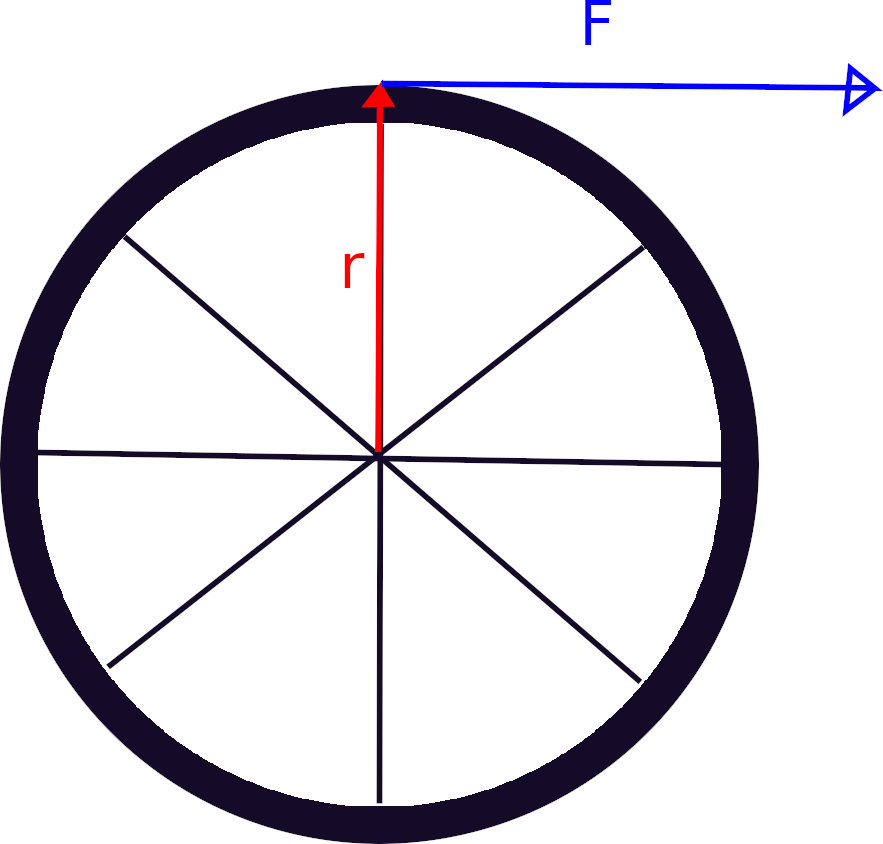
\includegraphics{"./Chapters/Ch09-RotationalMechanics/wheel.png"}
		\vspace{0.1in}
		
		We can use Equation \ref{equation:torquemagnitude} to determine the torque:
		\begin{equation*}
			|\vec{\tau}| = r \cdot F \cdot sin (\theta) = 0.1 \si{m} \cdot 10 \si{N} \cdot \sin( 90 \degree) = \boxed{1 \si{m \times N}}
		\end{equation*}
		
		The direction of the torque is given by the 1st right hand rule.  Your index finger points along the direction of $\vec{r}$.  Your middle finger bends 90 degrees and aligns with $\vec F$.  Your thumb shows the resulting direction of the torque: \textbf{into the page.}
		
	\end{mdframed}
	
	
	
	
	
	
	
	\subsection{Newton's Laws in a Rotational Setting}
	\index{Newton's Laws, Rotational}
	
	\subsubsection{Newton's First Law for Rotation}
	Objects in uniform rotational motion will remain in uniform rotational motion and objects at rotational rest will remain at rotational rest until acted upon by an external, unbalanced torque.  
	
	\subsubsection{Newton's Second Law for Rotation}
			\begin{mdframed}[backgroundcolor=orange!20!white]
		\begin{equation}
			\vec{\tau} = I \cdot \vec{\alpha}
			\label{equation:newtonssecondrotational}
		\end{equation}
	\end{mdframed}
	
	\subsubsection{Newton's Third Law for Rotation}
	For every torque, there is an equal opposite torque.
	
	
	\section{Angular Kinetic Energy}
	\index{Angular Kinetic Energy}
	\index{Kinetic Energy, Angular}
	
	\textbf{Angular Kinetic Energy}, sometimes called rotational kinetic energy, is energy of rotational motion.  An object that is only rotating - like a fan - has angular kinetic energy only.  An object that is rolling - like the wheel of a car - has both translational kinetic energy (found using $k = \frac{1}{2}mv^2$ ) and angular kinetic energy, found using:
	
				\begin{mdframed}[backgroundcolor=orange!20!white]
		\begin{equation}
			K = \frac{1}{2}I\omega^2
			\label{equation:rotationalkineticenergy}
		\end{equation}
	\end{mdframed}
	
	\newpage
	\section{Angular Momentum} \label{angularmomentum} \index{Angular Momentum}
	\subsection{The Definition of Angular Momentum}
	Angular momentum can be calculated using the formula: 
	 	\begin{mdframed}[backgroundcolor=orange!20!white]
		\begin{equation}
		\vec{L} = I \vec{\omega}
		\label{equation:angularmomentum}
				\end{equation}
	\end{mdframed}
where $\vec{L}$ is angular momentum, $I$ is the object's moment of Inertia and $\vec{\omega}$ is the object's angular velocity.  The SI units for angular momentum are  $\frac{kg m^2} {s} $.


\begin{mdframed}[backgroundcolor=blue!10!white]
	\begin{center}
		
		
		\textbf{Example \thesection.1}	
	\end{center}
	\vspace{0.1in}
	\textbf{Problem:} A bicycle wheel has a mass of 0.3 kg, and can be thought of as a thin ring with a radius of 0.33m. When the wheel is turning at a rate of 2 rotations per second, what its its angular momentum?
	\vspace{0.1in}
	
	\textbf{Solution:} 
	Begin by converting the angular velocity $\omega$ to appropriate units:
	\begin{equation*}
	\vec{\omega} = 2 \frac{rotations}{s} = 4\pi \frac{rad}{s}
	\end{equation*}
	
	Then calculate the moment of inertia.  Using the formula for a thin ring: 
	\begin{equation*}
	I  = mr^2 = 0.3 kg  (0.33m)^2 \approx 0.033 kg m^2
	\end{equation*}
	Finally, use equation \ref{equation:angularmomentum} to find the angular momentum. 
	
	\begin{equation*}
	\vec{L}  =  I \vec{\omega} = 0.011 kg m^2 \cdot 4\pi \frac{rad}{s} \approx \boxed{0.411 \frac{kg m^2}{s}}
	\end{equation*}
	
	
	
\end{mdframed}


	\subsection{Conservation of Angular Momentum}
 Just like linear momentum\footnote{see momentum in \cref{angularmomentum}}, angular momentum is a quantity that is conserved.  Thus, whatever angular momentum a closed system has in its initial state will be equal to the angular momentum the system has in its final state.  
 
 The classic example of the Law of Conservation of Momentum is an ice skater who enters a spin.  By changing the positioning of his or her arms and legs, an ice skater can change their moment of inertia.  When they bring their arms and legs closer to their axis of rotation, their moment of inertia decreases.  Since angular momentum is conserved, their angular velocity must increase as their moment of inertia decreases, and thus the ice skater is able to spin very fast. 
 
	
	

		


	


		
\chapter{Waves}
	\section{Fundamentals of Waves} \index{Waves}

	You have probably heard of waves in the context of the ocean, a lake, or other bodies of liquid.  Waves are also found in earthquakes, sound, light, and even at the stadium when people do ``the wave.''  A \textit{wave} is a distortion that transfers energy from one place to another without the permanent transfer of mass. 
	
	The material that a wave travels through is called a \textit{medium}. \index{Medium} \index{Waves, medium} For instance, the medium for an ocean wave is water, while the medium for light could be air, glass, water, or even empty space (no medium).  

		\subsection{Types of Waves}
	 Waves can be categorized into several basic types: 
	\begin{itemize}
		\item \textit{Transverse Waves} - are waves that are displaced perpendicular to the direction of travel.  For instance, ocean waves are a type of transverse wave because their displacement is vertical, though they travel horizontally.
		Normally, a transverse wave is drawn similar to the figure below:
		\begin{center}
		\begin{figure}[h]
			\centering
			\begin{tikzpicture}

				 \draw[thick, red]
				 (3,0) sin (4,1) cos (5,0) sin (6,-1) cos (7,0)
				 sin (8,1) cos (9,0) sin (10,-1) cos (11,0);	
			 \end{tikzpicture}
			 \caption{A simple transverse wave}
		\end{figure}
		\end{center}	
		
		\item \textit{Longitudinal Waves} - are waves that are displaced in the same direction as the direction of travel.  You can think of this as a compression, or shock wave that travels through a medium.  The places where a material is closer together than normal are called compressions, while places that are spaced farther apart are called rarefractions, as seen in figure \ref{tester}
		
		\begin{figure}[h]
			\centering
			\begin{tikzpicture}[font=\sffamily] 
			\begin{scope}[z={(70:1)},y={(110:1)},local bounding box=coil] 
			\draw plot[domain=0:14400,variable=\t,samples=1441,smooth] 
			({\t/1200+0.1*pi*sin(\t/20)},{-0.5*sin(\t)},{0.5*cos(\t)}); 
			\end{scope} 
			\path (coil.south west) -- (coil.south east) 
			node[pos=0.25,below]{Compression} node[pos=0.5,below]{Rarefraction}; 
			
		\end{tikzpicture} 


			
			\caption{A simple longitudinal wave}
			\label{tester}
		\end{figure}	
		
		\item \textit{Electromagnetic Waves} - are waves that are made up of oscillating electric and magnetic fields.  These are usually modeled as transverse waves, but they are just representations of the strength of the electric and magnetic fields. 
		
		
		\begin{figure}[h]
			\centering
			\begin{tikzpicture}[x={(-10:1cm)},y={(90:1cm)},z={(210:1cm)}]
			% Axes
			\draw (-1,0,0) node[above] {$x$} -- (5,0,0);
			\draw (0,0,0) -- (0,2,0) node[above] {$y$};
			\draw (0,0,0) -- (0,0,2) node[left] {$z$};
			% Propagation
			\draw[->,ultra thick] (5,0,0) -- node[above] {$c$} (6,0,0);
			% Waves
			\draw[thick] plot[domain=0:4.5,samples=200] (\x,{sin(deg(pi*\x))},0);
			\draw[gray,thick] plot[domain=0:4.5,samples=200] (\x,0,{cos(deg(pi*\x))});
			% Arrows
			\foreach \x in {0.1,0.3,...,4.4} {
				\draw[->,help lines] (\x,0,0) -- (\x,{sin(deg(pi*\x))},0);
				\draw[->,help lines] (\x,0,0) -- (\x,0,{cos(deg(pi*\x))});
			}
			% Labels
			\node[above right] at (0,1,0) {$\bm{E}$};
			\node[below] at (0,0,1) {$\bm{B}$};
			\end{tikzpicture}	
			\caption{An electromagnetic wave}
		\end{figure}
		 
		Electromagnetic waves are what make up the electromagnetic spectrum.  Radio waves, microwaves, infrared, visible light, ultraviolet, X-rays and $\gamma$-rays are all electromagnetic waves.  They are categorized into different types based on their frequency. 
		 
	\end{itemize}

	There are other types of waves, such as matter waves and gravitational waves that are beyond the scope of this text.  

\newpage
		\subsection{Basic Wave Characteristics and Vocabulary}
		
\begin{center}
	\begin{figure}[h]
		\centering
		\begin{tikzpicture}
		
		\draw[thick, red]
		(3,0) sin (4,1) cos (5,0) sin (6,-1) cos (7,0)
		sin (8,1) cos (9,0) sin (10,-1) cos (11,0) sin (12,1) cos (13,0);	
			\draw[-,ultra thick] (3,0) --  (13,0);
			\draw[->,ultra thick] (4,1) -- node[above] {$\lambda$} (8,1);
			\draw[->,ultra thick] (4,0) -- node[left] {$A$} (4,1);
			\draw[->,ultra thick] (6,0) -- node[left] {$A$} (6,-1);
		 	\draw [blue] (10,-1) circle[radius=2pt] node[below] {Trough};
		 	\fill[blue] (10,-1)  circle[radius=2pt];
	 		\draw [green] (12,1) circle[radius=2pt] node[above] {Crest};
		 	\fill[green] (12,1)  circle[radius=2pt];
		 	
		\end{tikzpicture}
		\caption{The measurements of a wave}
		\label{fig:wavemeasure}
	\end{figure}
\end{center}	
		
	\subsubsection{Extrema} \index{Crest} \index{Trough} \index{Wave, Crest} \index{Wave, Trough} 
	
	\textbf{Crests} are each of the highest points of a wave, and \textbf{troughs} (rhymes with coughs) are the lowest points of a wave, as seen in the diagram \ref{fig:wavemeasure}.  The word \textbf{extrema} refers to all crests and troughs, as they are the most extreme points of the wave. 
	
	\subsubsection{Amplitude} \index{Amplitude} \index{Wave, Amplitude} \textbf{Amplitude} measures how large or how strong a wave is.  It is measured from the center of a wave to one of the extrema - either upward to a crest, or downward to a trough.  For a physical, transverse wave, amplitude can be measured in meters.  The variable for amplitude is $A$.  For sound, we experience the amplitude of the wave as \textit{volume}, and for light, we experience it as \textit{brightness}.
	
	\subsubsection{Wavelength} \index{Wavelength}
	The \textbf{wavelength} of a wave is measured from any point to an identical point on the wave, along the axis of propagation.  Wavelength is measured in meters, and the symbol for wavelength is $\lambda$ (lambda).  The easiest way to measure wavelength is from crest to crest or from trough to trough. 
	
	\subsubsection{Period} \index{Period}
	The \textbf{period} of a wave measures how long it takes a wave to repeat itself.  It is measured in seconds, and uses the variable $T$.  
	
	\subsubsection{Frequency} \index{Frequency} 
	The \textbf{frequency} of a wave measures how many times a wave repeats itself in one second.  The symbol for frequency is $f$ and the units for frequency are $\frac{cycles}{second} $.  We give this unit the name \textit{hertz}, abbreviated Hz. For sound, we experience frequency as \textit{pitch}, and for light we experience frequency as \textit{color}. 
	
	\newpage
	
	The frequency of a wave and the period of a wave are inverses of each other.  Thus:
	
	
	\begin{mdframed}[backgroundcolor=orange!20!white]
		\begin{equation}
		f = \frac{1}{T}
		\label{equation:wavefrequency}
		\end{equation}
	\end{mdframed}	
	
	
	
	\begin{mdframed}[backgroundcolor=blue!10!white]
		\begin{center}
			
			
			\textbf{Example \thesection.1}	
		\end{center}
		
		\textbf{Problem: }A wave has a frequency of 102.1 MHz.  What is the period of the wave?
		\vspace{0.1in}
		
		\textbf{Solution:} 
		
		We know that $f = \SI{102.1}{\mega\hertz} $ Converting into scientific notation gives:
		 
		 	
		 \begin{equation*}
		 f = \SI{102.1}{\mega\hertz} = \SI{102.1e6}{\hertz} = \boxed{ \SI{1.021e8}{\hertz}}
		 \end{equation*}
		 
		
		Begin by using equation \ref{equation:wavefrequency}:
		
		
		\begin{equation*}
		f = \frac{1}{T}
		\end{equation*}
		
		Solving for $T$ yields:
		
		\begin{equation*}
			T = \frac{1}{f}
		\end{equation*}		
		
		Then, substitute numbers: 
		
		\begin{equation*}
		T = \frac{1}{\SI{1.021e8}{\hertz}} \approx \boxed{\SI{9.794e-9}{\s}}
		\end{equation*}		
		
	\end{mdframed}
	
	\subsection{Velocity of a Wave} \index{Velocity of a Wave} \index{Wave, Velocity}
	
	We already know from equation \ref{eqn:velocity} that the average velocity of any object is given by $\overrightarrow{v_{avg}} = \frac{\vec{d}}{\Delta t} $.  In the case of a wave, the time it takes the wave to repeat is the period, $T$, and distance the wave must move in order to repeat is one wavelength, $\lambda$.  Thus, $\overrightarrow{v_{avg}} = \frac{\vec{d}}{\Delta t} = \frac{\vec{\lambda}}{T}$.  Using equation \ref{equation:wavefrequency}, it can be proven that:
	
		\begin{mdframed}[backgroundcolor=orange!20!white]
		\begin{equation}
		v = f\lambda
		\label{equation:wavevelocity}
		\end{equation}
	\end{mdframed}	
	
	
	\newpage
	
	\begin{mdframed}[backgroundcolor=blue!10!white]
	\begin{center}
		
		
		\textbf{Example \thesection.2}	
	\end{center}
	
	\textbf{Problem: }An ocean wave has a period of 15 seconds, and is traveling at a speed of 2 meters per second.  How far is it from one crest of the wave to another? 
	
	\vspace{0.1in}
	
	\textbf{Solution:} 
	The question asks for the distance from one crest to another, which is the wavelength.  
	Given values:  \begin{center}
					$T = \SI{15}{\s}$

					$v = \SI[per-mode = symbol]{2}{\m\per\s} $
					\end{center}

	First, we use equation \ref{equation:wavefrequency} to find the frequency:
		\begin{equation*}
	f = \frac{1}{T} = \frac{1}{\SI{15}{s}} \approx \SI{0.067}{\s}
	\end{equation*}

	We now use equation \ref{equation:wavevelocity}:
	\begin{equation*}
		v = f\lambda
	\end{equation*}
	
	Solving for wavelength gives:
		\begin{equation*}
	\frac{v}{f} = \lambda
	\end{equation*}
	
	Substituting gives: 
	
	
	\begin{equation*}
	\lambda = \frac{v}{f} \approx \frac{\SI[per-mode = symbol]{2}{\m\per\s}}{\SI{.067}{\s}} \approx \boxed{\SI{30}{\m}}
	\end{equation*}		
	
\end{mdframed}
	
		
	
	\newpage
	
	
\section{The Doppler Effect} \index{Doppler Effect}
	We have all experienced a car driving past us while it is honking its horn.  As the car drives past, there is a significant change in the pitch of the horn.  In fact, when either the source of a wave or an observer of a wave is moving, it causes the observer's perception of the frequency of that wave to change.  This is called the \textbf{Doppler Effect}.  
	
	When the source of a wave moves \textit{toward} an observer, its frequency is shifted higher.  
	
	When the source of a wave moves \textit{away} from an observer, its frequency is shifted lower.  
	
	Likewise, when an observer moves \textit{toward} the source of a sound, its frequency is shifted higher.
	
	When an observer moves \textit{away} from a source of sound, its frequency is shifted lower.   
	
	The equation for the doppler effect is given by equation \ref{equation:dopplereffect}:
	
	
	
	
	
	
	
		\begin{mdframed}[backgroundcolor=orange!20!white]
		\begin{equation}
		f_{observed} = f_{source}(\frac{v_{wave} \pm v_{observer}}{v_{wave} \pm v_{source}})
		\label{equation:dopplereffect}
		\end{equation}
	\end{mdframed}	
	
	In this equation, do not consider the $\pm$ sign to represent both operations.  Instead, you must chose which operation to use based on the given situation.  In the numerator of the equation it is exactly what is expected: add for a higher frequency and subtract for a lower frequency.  In the denominator, it is backward - add for lower frequency, and subtract for higher frequency.  
	
	
	
	In the air, the speed of sound depends on air pressure, temperature, and even humidity.  The standard value for speed of sound in air is \textbf{343 m/s}, though in reality this number can change quite significantly depending on atmospheric conditions.  
	
	
	
	
	
	
	
	
	\begin{mdframed}[backgroundcolor=blue!10!white]
	\begin{center}
		
		
		\textbf{Example \thesection.1}	
	\end{center}
	
	\textbf{Problem: } A car's horn has a pitch of 550 Hz.  It is driving at 15 m/s toward a stationary observer.  \begin{enumerate}
		\item[a.] What is the frequency that the observer hears at the car approaches. 
		\item[b.] The car then passes the observer.  What is the frequency that the observer hears as the car travels away from him?  
		
	\end{enumerate}
	
	\vspace{0.1in}
	
	\textbf{Solution:} A car's horn produces sound, therefore the velocity of the wave is the speed of sound. 
  
	\underline{Part a:} Given values:  \begin{center}
		$f_{source} = \SI{550}{\Hz}$
		
		$v = \SI[per-mode = symbol]{343}{\m\per\s} $
		
		$v_{source} = \SI[per-mode = symbol]{15}{\m\per\s} $
		
		$v_{observer} = \SI[per-mode = symbol]{0}{\m\per\s} $
	\end{center}
	
	We can use equation \ref{equation:dopplereffect} to find the frequency the observer hears:

	\begin{equation*}
			f_{observed} = f_{source}(\frac{v_{wave} \pm v_{observer}}{v_{wave} \pm v_{source}})
	\end{equation*}
	
	In this case, the observer is not moving, so it does not matter whether we chose a plus or minus.  The source is moving toward the observer, causing the observer to hear a higher pitch.  Therefore, since the source is in the denominator, we chose a minus.  Substituting numbers and chosing correct signs gives:
	
	\begin{equation*}
	f_{observed} = \SI{550}{Hz}(\frac{\SI[per-mode = symbol]{343}{\m\per\s} + \SI[per-mode = symbol]{0}{\m\per\s}}{{\SI[per-mode = symbol]{343}{\m\per\s} - \SI[per-mode = symbol]{15}{\m\per\s}}})
	\end{equation*}
	
	
	
Evaluating this expression gives: 
	\begin{equation*}
	\boxed{f_{observed} \approx \SI{575.152}{Hz}}
	\end{equation*}
	
	
		\underline{Part b:} After the car has passed the observer, it is now traveling away from the observer.  Thus, the only change that needs to be made is that $v_{source}$ should now have a plus sign:
	
		\begin{equation*}
	f_{observed} = \SI{550}{Hz}(\frac{\SI[per-mode = symbol]{343}{\m\per\s} + \SI[per-mode = symbol]{0}{\m\per\s}}{{\SI[per-mode = symbol]{343}{\m\per\s} + \SI[per-mode = symbol]{15}{\m\per\s}}})
	\end{equation*}
	
	Evaluating this expression yields: 
	
		\begin{equation*}
	\boxed{f_{observed} \approx \SI{526.955}{Hz}}
	\end{equation*}
	
	
	
\end{mdframed}	
	
	
	
	
	
	
	
	
	
	
	
	
	
	
	
	
	
	
	\newpage
	
	
	
	
	
	
	
	
	
	
	
	
	
	
	
	
	
	
	
	
	
	
	
	
	
	
	
	
	
	
	
	
	
	
	
	
	
	
	
	
	
	
	
	
	
	
	\section{Waves and the Principle of Superposition} \index{Superposition} \index{Interference}
	
	The \textbf{Principle of Superposition} is the idea that waves can overlap.  Consider, for instance, a swimming pool where a light breeze creates ripples in the water as shown below: 
	
	
		\begin{figure}[h]
			\centering
			\resizebox{6in}{0.1in}{
		\begin{tikzpicture}
		\pgfmathdeclarefunction{S}{2}{\pgfmathparse{sin(deg(#1*#2*5.2))}}
	
		\begin{axis}
		[
		xtick={
			-6.28318, -4.7123889, -3.14159, -1.5708,
			1.5708, 3.14159, 4.7123889, 6.28318
		},
		xticklabels={
			$-2\pi$, $-\frac{3\pi}{2}$, $-\pi$, $\frac{\pi}{2}$,
			$\frac{\pi}{2}$, $\pi$, $\frac{3\pi}{2}$, $2\pi$
		},
		axis lines = none,
		grid=none,minor tick num=1,
		% xlabel=$x$,ylabel=$y$,
		tick align=inside,
		domain=-2*pi:2*pi,
		samples=200
		]
		\addplot [red,thick] {S(2,x)};
		\end{axis}
		\end{tikzpicture}
	}
	\caption{Ripples on a swimming pool}	
	\end{figure}
	
	You could also imagine in the same swimming pool on a calm day, a person could jump into the water creating waves that look similar to the ones below:
	
			\begin{figure}[h]
		\centering
		\resizebox{6in}{1in}{
			\begin{tikzpicture}
			\pgfmathdeclarefunction{S}{2}{\pgfmathparse{10*sin(deg(#1*#2/2))}}
			
			\begin{axis}
			[
			xtick={
				-6.28318, -4.7123889, -3.14159, -1.5708,
				1.5708, 3.14159, 4.7123889, 6.28318
			},
			xticklabels={
				$-2\pi$, $-\frac{3\pi}{2}$, $-\pi$, $\frac{\pi}{2}$,
				$\frac{\pi}{2}$, $\pi$, $\frac{3\pi}{2}$, $2\pi$
			},
			axis lines = none,
			grid=none,minor tick num=1,
			% xlabel=$x$,ylabel=$y$,
			tick align=inside,
			domain=-2*pi:2*pi,
			samples=200
			]
			\addplot [blue,thick] {S(2,x)};
			\end{axis}
			\end{tikzpicture}
		}
		
	\caption{Large waves in a swimming pool}
	\end{figure}


Thus, we can use the principle of superposition  to predict what the wave will look like should a person jump into the swimming pool on a day when there are ripples in the water.  By combining the two types of waves, we would see something like the figure below:

		\begin{figure}[h]
	\centering
	\resizebox{6in}{1in}{
		\begin{tikzpicture}
		\pgfmathdeclarefunction{S}{2}{\pgfmathparse{(sin(deg(#1*#2*6.2)))}}
			\pgfmathdeclarefunction{C}{2}{\pgfmathparse{10*sin(deg(#1*#2/2))}}
		
		\begin{axis}
		[
		xtick={
			-6.28318, -4.7123889, -3.14159, -1.5708,
			1.5708, 3.14159, 4.7123889, 6.28318
		},
		xticklabels={
			$-2\pi$, $-\frac{3\pi}{2}$, $-\pi$, $\frac{\pi}{2}$,
			$\frac{\pi}{2}$, $\pi$, $\frac{3\pi}{2}$, $2\pi$
		},
		axis lines = none,
		grid=none,minor tick num=1,
		% xlabel=$x$,ylabel=$y$,
		tick align=inside,
		domain=-2*pi:2*pi,
		samples=200
		]
		\addplot [violet,thick] {S(2,x)+C(2,x)};
		\end{axis}
		\end{tikzpicture}
	}
	
	\caption{Ripples and waves combine}
\end{figure}

\newpage

\section{Interference}
\subsection{Constructive Interference}


Sometimes, waves of approximately the same amplitude may overlap, causing the amplitude of the resulting wave to become larger.  This is called \textbf{Constructive Interference}: \index{Interference, Constructive}
\begin{figure}[h]
\newcolumntype{C}{ >{\centering\arraybackslash} m{1.5in} }
\newcolumntype{D}{ >{\centering\arraybackslash} m{.25in} }
\begin{tabular}{C D C D C }
	
	\resizebox{1in}{.25in}{
		\begin{tikzpicture}
		\pgfmathdeclarefunction{S}{2}{\pgfmathparse{(sin(deg(#1*#2)))}}
		
		
		\begin{axis}
		[
		xtick={
			-6.28318, -4.7123889, -3.14159, -1.5708,
			1.5708, 3.14159, 4.7123889, 6.28318
		},
		xticklabels={
			$-2\pi$, $-\frac{3\pi}{2}$, $-\pi$, $\frac{\pi}{2}$,
			$\frac{\pi}{2}$, $\pi$, $\frac{3\pi}{2}$, $2\pi$
		},
		axis lines = none,
		grid=none,minor tick num=1,
		% xlabel=$x$,ylabel=$y$,
		tick align=inside,
		domain=0:pi,
		samples=200
		]
		\addplot [red,thick] {S(2,x)};
		\end{axis}
		\end{tikzpicture}
	}
	
	&
	+
	&
	
	\resizebox{1in}{.5in}{
		\begin{tikzpicture}
		\pgfmathdeclarefunction{S}{2}{\pgfmathparse{(sin(deg(#1*#2)))}}
		
		
		\begin{axis}
		[
		xtick={
			-6.28318, -4.7123889, -3.14159, -1.5708,
			1.5708, 3.14159, 4.7123889, 6.28318
		},
		xticklabels={
			$-2\pi$, $-\frac{3\pi}{2}$, $-\pi$, $\frac{\pi}{2}$,
			$\frac{\pi}{2}$, $\pi$, $\frac{3\pi}{2}$, $2\pi$
		},
		axis lines = none,
		grid=none,minor tick num=1,
		% xlabel=$x$,ylabel=$y$,
		tick align=inside,
		domain=0:pi,
		samples=200
		]
		\addplot [red,thick] {S(2,x)};
		\end{axis}
		\end{tikzpicture}
	}
	&
	$\longrightarrow$
	&
	
	\resizebox{1in}{.75in}{
		\begin{tikzpicture}
		\pgfmathdeclarefunction{S}{2}{\pgfmathparse{(sin(deg(#1*#2)))}}
		
		
		\begin{axis}
		[
		xtick={
			-6.28318, -4.7123889, -3.14159, -1.5708,
			1.5708, 3.14159, 4.7123889, 6.28318
		},
		xticklabels={
			$-2\pi$, $-\frac{3\pi}{2}$, $-\pi$, $\frac{\pi}{2}$,
			$\frac{\pi}{2}$, $\pi$, $\frac{3\pi}{2}$, $2\pi$
		},
		axis lines = none,
		grid=none,minor tick num=1,
		% xlabel=$x$,ylabel=$y$,
		tick align=inside,
		domain=0:pi,
		samples=200
		]
		\addplot [red,thick] {S(2,x)};
		\end{axis}
		\end{tikzpicture}
	}
\end{tabular}
\caption{Constructive interference}
\end{figure}

In order for constructive interference to happen, the two waves must be \textit{in phase} - that is, the displacement of the waves must be in the same direction. 







\subsection{Destructive Interference}

	At other times, waves may overlap while they are \textbf{out of phase} - that is, their displacement is in opposite directions, causing the wave to become smaller. This is called \textbf{destructive interference}.   \index{Interference, Destructive}

	
	\begin{figure}[h]
		\newcolumntype{C}{ >{\centering\arraybackslash} m{1.5in} }
		\newcolumntype{D}{ >{\centering\arraybackslash} m{.25in} }
		\begin{tabular}{C D C D C }
			
			\resizebox{1in}{.75in}{
				\begin{tikzpicture}
				\pgfmathdeclarefunction{S}{2}{\pgfmathparse{(sin(deg(#1*#2)))}}
				
				
				\begin{axis}
				[
				xtick={
					-6.28318, -4.7123889, -3.14159, -1.5708,
					1.5708, 3.14159, 4.7123889, 6.28318
				},
				xticklabels={
					$-2\pi$, $-\frac{3\pi}{2}$, $-\pi$, $\frac{\pi}{2}$,
					$\frac{\pi}{2}$, $\pi$, $\frac{3\pi}{2}$, $2\pi$
				},
				axis lines = none,
				grid=none,minor tick num=1,
				% xlabel=$x$,ylabel=$y$,
				tick align=inside,
				domain=0:pi,
				samples=200
				]
				\addplot [red,thick] {S(2,x)};
				\end{axis}
				\end{tikzpicture}
			}
			
			&
			+
			&
			
			\resizebox{1in}{1in}{
				\begin{tikzpicture}
				\pgfmathdeclarefunction{S}{2}{\pgfmathparse{(sin(deg(#1*#2)))}}
				
				
				\begin{axis}
				[
				xtick={
					-6.28318, -4.7123889, -3.14159, -1.5708,
					1.5708, 3.14159, 4.7123889, 6.28318
				},
				xticklabels={
					$-2\pi$, $-\frac{3\pi}{2}$, $-\pi$, $\frac{\pi}{2}$,
					$\frac{\pi}{2}$, $\pi$, $\frac{3\pi}{2}$, $2\pi$
				},
				axis lines = none,
				grid=none,minor tick num=1,
				% xlabel=$x$,ylabel=$y$,
				tick align=inside,
				domain=0:pi,
				samples=200
				]
				\addplot [red,thick] {-S(2,x)};
				\end{axis}
				\end{tikzpicture}
			}
			&
			$\longrightarrow$
			&
			
			\resizebox{1in}{.25in}{
				\begin{tikzpicture}
				\pgfmathdeclarefunction{S}{2}{\pgfmathparse{(sin(deg(#1*#2)))}}
				
				
				\begin{axis}
				[
				xtick={
					-6.28318, -4.7123889, -3.14159, -1.5708,
					1.5708, 3.14159, 4.7123889, 6.28318
				},
				xticklabels={
					$-2\pi$, $-\frac{3\pi}{2}$, $-\pi$, $\frac{\pi}{2}$,
					$\frac{\pi}{2}$, $\pi$, $\frac{3\pi}{2}$, $2\pi$
				},
				axis lines = none,
				grid=none,minor tick num=1,
				% xlabel=$x$,ylabel=$y$,
				tick align=inside,
				domain=0:pi,
				samples=200
				]
				\addplot [red,thick] {-S(2,x)};
				\end{axis}
				\end{tikzpicture}
			}
		\end{tabular}
		\caption{Destructive Interference}
	\end{figure}
	
	
	
	
	If two waves are displaced by the same amount in opposite directions, they can even cancel out completely.  This would be \textbf{perfectly destructive interference}: 
	
		\begin{figure}[h]
		\newcolumntype{C}{ >{\centering\arraybackslash} m{1.5in} }
		\newcolumntype{D}{ >{\centering\arraybackslash} m{.25in} }
		\begin{tabular}{C D C D C }
			
			\resizebox{1in}{.75in}{
				\begin{tikzpicture}
				\pgfmathdeclarefunction{S}{2}{\pgfmathparse{(sin(deg(#1*#2)))}}
				
				
				\begin{axis}
				[
				xtick={
					-6.28318, -4.7123889, -3.14159, -1.5708,
					1.5708, 3.14159, 4.7123889, 6.28318
				},
				xticklabels={
					$-2\pi$, $-\frac{3\pi}{2}$, $-\pi$, $\frac{\pi}{2}$,
					$\frac{\pi}{2}$, $\pi$, $\frac{3\pi}{2}$, $2\pi$
				},
				axis lines = none,
				grid=none,minor tick num=1,
				% xlabel=$x$,ylabel=$y$,
				tick align=inside,
				domain=0:pi,
				samples=200
				]
				\addplot [red,thick] {S(2,x)};
				\end{axis}
				\end{tikzpicture}
			}
			
			&
			+
			&
			
			\resizebox{1in}{1in}{
				\begin{tikzpicture}
				\pgfmathdeclarefunction{S}{2}{\pgfmathparse{(sin(deg(#1*#2)))}}
				
				
				\begin{axis}
				[
				xtick={
					-6.28318, -4.7123889, -3.14159, -1.5708,
					1.5708, 3.14159, 4.7123889, 6.28318
				},
				xticklabels={
					$-2\pi$, $-\frac{3\pi}{2}$, $-\pi$, $\frac{\pi}{2}$,
					$\frac{\pi}{2}$, $\pi$, $\frac{3\pi}{2}$, $2\pi$
				},
				axis lines = none,
				grid=none,minor tick num=1,
				% xlabel=$x$,ylabel=$y$,
				tick align=inside,
				domain=0:pi,
				samples=200
				]
				\addplot [red,thick] {-S(2,x)};
				\end{axis}
				\end{tikzpicture}
			}
			&
			$\longrightarrow$
			&
			
			\resizebox{1in}{.01in}{
				\begin{tikzpicture}
				\pgfmathdeclarefunction{S}{2}{\pgfmathparse{(sin(deg(#1*#2)))}}
				
				
				\begin{axis}
				[
				xtick={
					-6.28318, -4.7123889, -3.14159, -1.5708,
					1.5708, 3.14159, 4.7123889, 6.28318
				},
				xticklabels={
					$-2\pi$, $-\frac{3\pi}{2}$, $-\pi$, $\frac{\pi}{2}$,
					$\frac{\pi}{2}$, $\pi$, $\frac{3\pi}{2}$, $2\pi$
				},
				axis lines = none,
				grid=none,minor tick num=1,
				% xlabel=$x$,ylabel=$y$,
				tick align=inside,
				domain=0:pi,
				samples=200
				]
				\addplot [red,thick] {0 * S(2,x)};
				\end{axis}
				\end{tikzpicture}
			}
		\end{tabular}
		\caption{Perfectly Destructive Interference}
	\end{figure}
	
	
	
	
	
	
	
	
	

	

	


	
\chapter{Optics}
	\index{Optics} Optics is the study of light and how that light interacts with matter.  There are two general fields of Optics: \textit{Geometric Optics} and \textit{Physical Optics}. Geometric optics studies how rays of light travel, while physical optics studies how multiple rays of light interact as waves.  
	
	An important constant in the field of optics is the speed of light.  The speed of light in empty space is exactly:	\index{Speed of Light}
	\begin{mdframed}[backgroundcolor=green!20!white]
		\begin{equation*}
		c = \SI{299792458}{m/s}
		\label{equation:speedoflight}
		\end{equation*}
	\end{mdframed}	
	
	The symbol used is \textit{c} because the speed of light is constant in all frames of reference.  This fact will be discussed in more detail in \color{red} (Insert REFERENCE  HERE.) \color{black} You will often see this number rounded to $2.998 \times 10^8$ m/s or even $3.0 \times 10^8 $m/s.
	
	
	
	
	\section{Geometric Optics} \index{Geometric Optics}
	
	While light in empty space always travels at the same speed, $c$, light can be slowed down when it travels through a medium.  This leads to some phenomena that we may encounter in everyday life.  
	

	\subsection{Refraction} \index{Refraction}
		
	\textit{Refraction} is a phenomenon associated with how light changes direction as it moves from one medium to another, due to the change in the speed that light travels at in each of the media.  This is often demonstrated by looking at a pencil in a glass of water, or a fish in a pond.  
	
	\subsubsection{The Index of Refraction}
	The index of refraction \index{Index of Refraction} is the ratio of the speed of light in a vacuum to the speed of light in a material.  It can be calculated as follows:
	
	
		
	\begin{mdframed}[backgroundcolor=orange!20!white]
		
		\begin{equation}
		n \equiv \frac{c}{v_m}
		\label{equation:indexofrefraction}
		\end{equation}
	\end{mdframed}
 
 where $n$ is the index of refraction, $c$ is the speed of light in empty space, and $v_m$ is the speed of light in the material.  
 
 
 	\begin{mdframed}[backgroundcolor=blue!10!white]
 	\begin{center}	
 		\textbf{Example \thesection.1}	
 	\end{center}
 	
 	\textbf{Problem: } Light travels at a speed of $2.254 \times 10^8$ m/s in water.  What is the index of refraction of water? 
 	
 	\textbf{Solution:} Using the definition of index of refraction, we find:
 	
 	\begin{equation}
			n \equiv \frac{c}{v_m} = \frac{2.997 \times 10^8 \, \si{m/s}}{2.254 \times 10^8 \, \si{m/s}} = 1.330
 	\end{equation}
 \end{mdframed}
 
 You may notice that the index of refraction is unitless, since all units cancel in the calculation.   A list of indices of refraction can be found in Appendix \ref{tab:refraction} on  \cpageref{tab:refraction}.
 
 
	
		\subsubsection{Snell's Law} \index{Snell's Law}
		\textit{Snell's Law}, named for the Dutch physicist Willebrord Snell, explains that light always takes the path of least time between two points.  When light travels in a single medium of constant optical density, it travels in a straight line.  However, when light changes medium, it will change direction.  	
		
		
		There are several components and measurements that should be included on a diagram in this situation.  		
		\begin{itemize}
			 \setlength\itemsep{0em}
			\item The \textit{interface} is the boundary where the two materials meet.  
			\item The \textit{normal} is an imaginary line perpendicular to the surface.  
			\item The \textit{incident ray} is the ray of light that is traveling toward the interface.
			\item The \textit{refracted ray} is the ray of light traveling away from the interface.  
			\item The \textit{incident angle}, $\theta_i$ is the angle between the incident ray and the normal.
			\item The \textit{refracted angle} $\theta_r$ is the angle between the refracted ray and the normal.  			
		\end{itemize}
		
		
		A diagram that shows a ray of light traveling from air into water might look like this:
		\begin{figure}[H]
			

		\begin{center}
			

		\begin{tikzpicture}[thick,scale=0.5, every node/.style={scale=0.5}]
		
		% define coordinates
		\coordinate (O) at (0,0) ;
		\coordinate (A) at (0,4) ;
		\coordinate (B) at (0,-4) ;
		
		% media
		\fill[blue!15!,opacity=.3] (-4,0) rectangle (4,4);
		\fill[blue!60!,opacity=.3] (-4,0) rectangle (4,-4);
		\node[right] at (2,2) {Air};
		\node[right] at (2,-2) {Water};
		\node[] at (2,0) {Interface};
	
		
		% axis
		\draw[dash pattern=on5pt off3pt] (A) -- (B) ;

		
		% rays
		\draw[red,ultra thick,reverse directed] (O) -- (130:5.2);
		\draw[red,directed,ultra thick] (O) -- (-70:4.24);
		
		% angles
		\draw (0,1) arc (90:130:1);
		\draw (0,-1.4) arc (270:290:1.4) ;
		\node[] at (280:1.8)  {$\theta_{r}$};
		\node[] at (110:1.4)  {$\theta_{i}$};
		
		\end{tikzpicture}
		\caption{A diagram of light traveling from air into water.}
		\end{center}
		\end{figure}		
		
		In a diagram such as above, it can be seen that the path of least time is given by the following mathematical representation of Snell's Law: 
		
		
			\begin{mdframed}[backgroundcolor=orange!20!white]
			
			\begin{equation}
			n_i \sin(\theta_{i}) = n_r \sin(\theta_{r})
			\label{equation:snellslaw}
			\end{equation}
		\end{mdframed}
	
	
		 	\begin{mdframed}[backgroundcolor=blue!10!white]
			\begin{center}	
				\textbf{Example \thesection.2}	
			\end{center}
			
			\textbf{Problem: } Light travels from water (n=1.33) into diamond (n=2.417).  If the angle of incidence is $45 \degree$, what is the refracted angle?  
			
			\textbf{Solution:} Begin by drawing a (partial) diagram:
			
			\begin{center}
			
			
			
			\begin{tikzpicture} [thick,scale=0.5, every node/.style={scale=0.5}]
			
			% define coordinates
			\coordinate (O) at (0,0) ;
			\coordinate (A) at (0,4) ;
			\coordinate (B) at (0,-4) ;
			
			% media
			\fill[blue!15!,opacity=.3] (-4,0) rectangle (4,4);
			\fill[gray!60!,opacity=.3] (-4,0) rectangle (4,-4);
			\node[right] at (2,2) {Water, n=1.33};
			\node[right] at (2,-2) {Diamond, n=2.417};

			
			
			% axis
			\draw[dash pattern=on5pt off3pt] (A) -- (B) ;
			
			
			% rays
			\draw[red,ultra thick,reverse directed] (O) -- (135:5.2);
			
			% angles
			\draw (0,1) arc (90:135:1);


			\node[] at (110:1.4)  {$45 \degree$};
			
			\end{tikzpicture}
			
			
		\end{center}
			
			Snell's law states:
			
			\begin{equation*}
			n_i \sin(\theta_{i}) = n_r \sin(\theta_{r})
			\end{equation*}
	
		
		Solving this for $\theta_{r}$ yields:
		
		\begin{equation}
	  \theta_{r} =	\sin^{-1}(\frac{n_i \sin(\theta_{i})}{n_r}) = \sin^{-1}(\frac{1.33 \sin(45 \degree)}{2.417}) \approx \boxed{22.898 \degree}
		\end{equation}
		
		The completed diagram would look like this:
		
			
		\begin{center}
			
			
			
			\begin{tikzpicture}[thick,scale=0.5, every node/.style={scale=0.5}]
			
			% define coordinates
			\coordinate (O) at (0,0) ;
			\coordinate (A) at (0,4) ;
			\coordinate (B) at (0,-4) ;
			
			% media
			\fill[blue!15!,opacity=.3] (-4,0) rectangle (4,4);
			\fill[gray!60!,opacity=.3] (-4,0) rectangle (4,-4);
			\node[right] at (2,2) {Water, n=1.33};
			\node[right] at (2,-2) {Diamond, n=2.417};
			
			
			
			% axis
			\draw[dash pattern=on5pt off3pt] (A) -- (B) ;
			
			
			% rays
			\draw[red,ultra thick,reverse directed] (O) -- (135:5.2);
			\draw[red,directed,ultra thick] (O) -- (-67.1:4.24);
			
			% angles
			\draw (0,1) arc (90:135:1);
			\draw (0,-2.5) arc (270:292.8:2.5) ;
			
			
			\node[] at (110:1.4)  {$45 \degree$};
			\node[] at (282:3.4)  {$22.898 \degree$};
			
			\end{tikzpicture}
			
			
		\end{center}
		
				
		
	
		
		
		
		
		\end{mdframed}	
	\newpage
		
		\paragraph{Total Internal Reflection} \index{Total Internal Reflection}
			In the specific case that light is traveling from a material with a higher index of refraction into a material with a lower index of refraction, the refracted angle will be larger than the incident angle.  In this case, it is possible that the refracted angle could refract at exactly $90 \degree$.  The incident angle that causes a ray to be refracted at $90 \degree$ is called the \textit{critical angle}\index{critical angle}.  If the angle of the incident ray exceeds the critical angle, the ray does not refract out of the material.  Instead, it reflects back into the material.
			
		\begin{figure}[H]
			

		\begin{center}
		
		\begin{tabular}{c c c}
					
					Refraction & Critical Angle & Total Internal Reflection \\
					
					
						\begin{tikzpicture}[thick,scale=0.5, every node/.style={scale=0.5}]
					
					% define coordinates
					\coordinate (O) at (0,0) ;
					\coordinate (A) at (0,4) ;
					\coordinate (B) at (0,-4) ;
					
					% media
					\fill[gray!25!,opacity=.3] (-4,0) rectangle (4,4);
					\fill[blue!5!,opacity=.3] (-4,0) rectangle (4,-4);
					\node[right] at (2,2) {Glass, n=1.517};
					\node[right] at (2,-2) {Air, n=1};
					
					
					
					% axis
					\draw[dash pattern=on5pt off3pt] (A) -- (B) ;
					
					
					% rays
					\draw[red,ultra thick,reverse directed] (O) -- (125:5.2);
					\draw[red,directed,ultra thick] (O) -- (330:4.5);
					
					% angles
					\draw (0,1) arc (90:125:1);
					\draw (0,-1) arc (270:330:1) ;
					
					
					\node[] at (110:1.9)  {$35 \degree$};
					\node[] at (110:2.5)  {$\theta_{i}$=};
					\node[] at (300:1.5)  {$60.47 \degree$};
					
					\end{tikzpicture} 
					
					&
	\begin{tikzpicture}[thick,scale=0.5, every node/.style={scale=0.5}]
	
	% define coordinates
	\coordinate (O) at (0,0) ;
	\coordinate (A) at (0,4) ;
	\coordinate (B) at (0,-4) ;
	
	% media
	\fill[gray!25!,opacity=.3] (-4,0) rectangle (4,4);
	\fill[blue!5!,opacity=.3] (-4,0) rectangle (4,-4);
	\node[right] at (2,2) {Glass, n=1.517};
	\node[right] at (2,-2) {Air, n=1};
	
	
	
	% axis
	\draw[dash pattern=on5pt off3pt] (A) -- (B) ;
	
	
	% rays
	\draw[red,ultra thick,reverse directed] (O) -- (131:5.2);
	\draw[red,directed,ultra thick] (O) -- (0:4);
	
	% angles
	\draw (0,1) arc (90:135:1);
	\draw (0,-1) arc (270:360:1) ;
	
	
	\node[] at (110:1.9)  {$41.239 \degree$};
		\node[] at (110:2.5)  {$\theta_{c}$=};
	\node[] at (315:1.4)  {$90 \degree$};
	
	\end{tikzpicture} 
	
	
	& 
	
		\begin{tikzpicture}[thick,scale=0.5, every node/.style={scale=0.5}]
	
	% define coordinates
	\coordinate (O) at (0,0) ;
	\coordinate (A) at (0,4) ;
	\coordinate (B) at (0,-4) ;
	
	% media
	\fill[gray!25!,opacity=.3] (-4,0) rectangle (4,4);
	\fill[blue!5!,opacity=.3] (-4,0) rectangle (4,-4);
	\node[right] at (2,2) {Glass, n=1.517};
	\node[right] at (2,-2) {Air, n=1};
	
	
	
	% axis
	\draw[dash pattern=on5pt off3pt] (A) -- (B) ;
	
	
	% rays
	\draw[red,ultra thick,reverse directed] (O) -- (131:5.2);
	\draw[red,directed,ultra thick] (O) -- (45:5.2);
	
	% angles
	\draw (0,1) arc (90:135:1);
	\draw (0,1) arc (90:45:1) ;
	
	
	\node[] at (110:1.9)  {$45 \degree$};
	\node[] at (110:2.5)  {$\theta_{i}$=};
	\node[] at (65:1.4)  {$45 \degree$};
	
	\end{tikzpicture} 
	
	
	
	
	
	 \\
\end{tabular}
	
			\end{center}
		\caption{Total internal reflection occurs when the critical angle is exceeded.}
\end{figure}					




\begin{mdframed}[backgroundcolor=blue!10!white]
	\begin{center}	
		\textbf{Example \thesection.3}	
	\end{center}
	
	\textbf{Problem:} Light travels from glass (n=1.517) into water (n=1.33).  Calculate the critical angle, and draw a diagram of the situation. 
	\vspace{0.1in}
	
	\textbf{Solution:} We know that the refracted ray must travel at a $90 \degree$ angle to the normal, so $\theta_{r} = 90 \degree$.  
	
	Snell's Law states:
	
	\begin{equation*}
		n_i \sin(\theta_i) = n_r \sin(\theta_{r})
	\end{equation*}
	
	Solving for $\theta_{i}$ gives:
	
	
	\begin{equation}
	\theta_{i} = \sin^{-1} (\frac{n_r \sin(\theta_{r})}{n_i}) = \sin^{-1} (\frac{1.33 \sin(90)}{1.517}) \approx \boxed{ 61.250 \degree}
	\end{equation}
	
	
	The corresponding diagram should look like the following:
	\begin{center}
		

	
		\begin{tikzpicture}[thick,scale=0.5, every node/.style={scale=0.5}]
	
	% define coordinates
	\coordinate (O) at (0,0) ;
	\coordinate (A) at (0,4) ;
	\coordinate (B) at (0,-4) ;
	
	% media
	\fill[gray!25!,opacity=.3] (-4,0) rectangle (4,4);
	\fill[blue!25!,opacity=.3] (-4,0) rectangle (4,-4);
	\node[right] at (2,2) {Glass, n=1.517};
	\node[right] at (2,-2) {water, n=1.33};
	
	
	
	% axis
	\draw[dash pattern=on5pt off3pt] (A) -- (B) ;
	
	
	% rays
	\draw[red,ultra thick,reverse directed] (O) -- (151:5.2);
	\draw[red,directed,ultra thick] (O) -- (0:4);
	
	% angles
	\draw (0,1) arc (90:151:1);
	\draw (0,-1) arc (270:360:1) ;
	
	
	\node[] at (110:1.9)  {$61.250 \degree$};
	\node[] at (110:2.5)  {$\theta_{c}$=};
	\node[] at (315:1.4)  {$90 \degree$};
	
	\end{tikzpicture} 
	
	\end{center}	
	
\end{mdframed}

		\subsubsection{Lenses} \index{Lens}

There are two basic types of lenses that are discussed in this text: \index{Lens}
\begin{itemize}
	\item \textit{Convex} lenses, sometimes called \textit{converging} lenses are larger in the center than at the edges.  These lenses are often used as magnifying glasses.  	

	\begin{figure} [H]

		\begin{center}
		\begin{tikzpicture}
		%sets the lens shape
		\pgfmathsetmacro{\lensRadius}{2}
		\pgfmathsetmacro{\lensHeight}{1}
		\pgfmathsetmacro{\startAngle}{asin(\lensHeight/\lensRadius)}
		
		%draws the lens
		\draw (0,\lensHeight) arc[start angle=180-\startAngle,delta angle=2*\startAngle,radius=\lensRadius];
		\draw (0,\lensHeight) arc[start angle=\startAngle,delta angle=-2*\startAngle,radius=\lensRadius];
		
		%draws a dotted line through the middle of the lens
		%\draw[dash pattern=on5pt off3pt] (0,-1) -- (0,1) ;
		\end{tikzpicture}
				\caption{A Simple diagram representation of a convex lens}
	\end{center}
	\end{figure}



\item \textit{Concave} lenses, sometimes called \textit{diverging} lenses are larger at the edges than the center.  They are found in lenses for near-sightedness.  

\begin{center}
	\begin{figure}[H]
		\begin{center}

	\begin{tikzpicture}
	

	
	\draw [thick, fill=white] (-.4,-.9) 	arc[start angle=-35, end angle=35,radius=1.5];
	\draw [thick, fill=white] (.4,-.9) 	arc[start angle=215, end angle=145,radius=1.5];
	
	\begin{scope}[>=latex]
	\draw [] (-.4,-.9) -- (.4,-.9);
	\draw [] (-.4,.82) -- (.4,.82);
	\end{scope}

		\end{tikzpicture}
				\caption{A Simple diagram representation of a concave lens}
				\end{center}
	\end{figure}
\end{center}

\end{itemize}


\paragraph{Convex Lenses} \index{Lens, Convex} \index{Convex Lens}

When parallel rays of light strike a convex lens, the light can be focused into a very small area.  The point at which the light is focused is called the focal point \index{Focal Point}.  

	\begin{figure} [H]
	
	\begin{center}
		\begin{tikzpicture}
		%sets the lens shape
		\pgfmathsetmacro{\lensRadius}{2}
		\pgfmathsetmacro{\lensHeight}{1}
		\pgfmathsetmacro{\startAngle}{asin(\lensHeight/\lensRadius)}
		
		%draws the lens
		\draw (0,\lensHeight) arc[start angle=180-\startAngle,delta angle=2*\startAngle,radius=\lensRadius];
		\draw (0,\lensHeight) arc[start angle=\startAngle,delta angle=-2*\startAngle,radius=\lensRadius];
		
		%draws a dotted line through the middle of the lens
		\draw[dash pattern=on5pt off3pt] (0,-1) -- (0,1) ;
		
		%incident Rays
		\draw[red,directed] (-5,.8) -- (0,.8) ;
		\draw[red,directed] (-5,.4) -- (0,.4) ;
		\draw[red,directed] (-5,.0) -- (0,.0) ;
		\draw[red,directed] (-5,-.4) -- (0,-.4) ;
		\draw[red,directed] (-5,-.8) -- (0,-.8) ;
		
		%Refracted rays
		\draw[red,directed] (0,.8) -- (5,-.8) ;
		\draw[red,directed] (0,.4) -- (5,-.4) ;
		\draw[red,directed] (0,.0) -- (5,.0) ;
		\draw[red,directed] (0,-.4) -- (5,.4) ;
		\draw[red,directed] (0,-.8) -- (5,.8) ;
		
		\node[below] at (2.5,0) {$f$};
		
		\end{tikzpicture}
		\caption{Light focused by a convex lens.  The focal point is labeled $f$.}
	\end{center}
\end{figure}

The distance from the center of the lens to the focal point is called the \textit{Focal Length.} \index{Focal Length}  Because light call pass through the lens either way, lenses have two focal points, both equidistant from the center of the lens.  

\subparagraph{Image Formation with Convex Lenses}
When a lens interacts with an object, an image is normally formed.  There are two often-used methods for determining where images form: \textit{Ray Tracing} and use of \textit{the lens equation.}

The method of ray tracing is performed in the following example: 

\begin{mdframed}[backgroundcolor=blue!10!white]
	\begin{center}	
		\textbf{Example \thesection.}	
	\end{center}
	
	\textbf{Problem:} A 1-cm tall object is placed 4 cm to the left of a lens of focal length $f=2 \si{cm}$.  Use ray-tracing to determine the position, size, and orientation of the image.  

\textbf{Solution}: 


\begin{enumerate}
	\item Begin by drawing a horizontal line across your paper.  This is your optical axis: 
	\vspace{.5 in}
	\begin{center}
		

	\begin{tikzpicture}
	%optical axis
	\draw (-7,0) -- (7,0);
	\end{tikzpicture}
		\end{center}
	\vspace{.5 in}
	
	
	
	\item Draw a lens on the optical axis.  Use a dotted line to represent the center of the lens.  
	

	\begin{center}
		
		
		\begin{tikzpicture}
		%draws the optical axis
		\draw (-7,0) -- (7,0);
		
			
		%sets the lens shape
		\pgfmathsetmacro{\lensRadius}{8}
		\pgfmathsetmacro{\lensHeight}{2}
		\pgfmathsetmacro{\startAngle}{asin(\lensHeight/\lensRadius)}
		
		%draws the lens
		\draw (0,\lensHeight) arc[start angle=180-\startAngle,delta angle=2*\startAngle,radius=\lensRadius];
		\draw (0,\lensHeight) arc[start angle=\startAngle,delta angle=-2*\startAngle,radius=\lensRadius];
		
		%draws a dotted line through the middle of the lens
		\draw[dash pattern=on5pt off3pt] (0,-2) -- (0,2) ;		
		\end{tikzpicture}
	\end{center}

	\item Measure and label focal points from the center of the lens, along the optical axis, and draw the object as an arrow with its base on the optical axis.
		\begin{center}
		
		
		\begin{tikzpicture}[place/.style={circle,fill=red}]
		%draws the optical axis
		\draw (-7,0) -- (7,0);
		
		
		%sets the lens shape
		\pgfmathsetmacro{\lensRadius}{8}
		\pgfmathsetmacro{\lensHeight}{2}
		\pgfmathsetmacro{\startAngle}{asin(\lensHeight/\lensRadius)}
		
		%draws the lens
		\draw (0,\lensHeight) arc[start angle=180-\startAngle,delta angle=2*\startAngle,radius=\lensRadius];
		\draw (0,\lensHeight) arc[start angle=\startAngle,delta angle=-2*\startAngle,radius=\lensRadius];
		
		%draws a dotted line through the middle of the lens
		\draw[dash pattern=on5pt off3pt] (0,-2) -- (0,2) ;	
		
		%draws focal points
		\node (n1) at (-2,0) [place] {};	
		\node (n21) at (2,0) [place] {};
		
			
		
		%draws object
		\draw [->,ultra thick] (-4,0) --(-4,1);
		\end{tikzpicture}
	\end{center}
	
\item The first ray of light will begin on the left of the diagram, graze the top of the object, and continue to the center of the lens.  It will then be directed down, through the far focal point.  

		\begin{center}
	
	
	\begin{tikzpicture}[place/.style={circle,fill=red}]
	%draws the optical axis
	\draw (-7,0) -- (7,0);
	
	
	%sets the lens shape
	\pgfmathsetmacro{\lensRadius}{8}
	\pgfmathsetmacro{\lensHeight}{2}
	\pgfmathsetmacro{\startAngle}{asin(\lensHeight/\lensRadius)}
	
	%draws the lens
	\draw (0,\lensHeight) arc[start angle=180-\startAngle,delta angle=2*\startAngle,radius=\lensRadius];
	\draw (0,\lensHeight) arc[start angle=\startAngle,delta angle=-2*\startAngle,radius=\lensRadius];
	
	%draws a dotted line through the middle of the lens
	\draw[dash pattern=on5pt off3pt] (0,-2) -- (0,2) ;	
	
	%draws focal points
	\node (n1) at (-2,0) [place] {};	
	\node (n21) at (2,0) [place] {};
	
	
	
	%draws object
	\draw [->, ultra thick] (-4,0) --(-4,1);
	
	
	%First Ray
	\draw [directed, ultra thick,red] (-7,1) --(0,1);
	\draw [directed, ultra thick,red] (0,1) --(6,-2);	
	\end{tikzpicture}
\end{center}

\item The second ray of light will graze the top of the object, pass through the near focal point, continuing until it hits the center of the lens.  There, the ray will be directed parallel to the optical axis.  

		\begin{center}
	
	
	\begin{tikzpicture}[place/.style={circle,fill=red}]
	%draws the optical axis
	\draw (-7,0) -- (7,0);
	
	
	%sets the lens shape
	\pgfmathsetmacro{\lensRadius}{8}
	\pgfmathsetmacro{\lensHeight}{2}
	\pgfmathsetmacro{\startAngle}{asin(\lensHeight/\lensRadius)}
	
	%draws the lens
	\draw (0,\lensHeight) arc[start angle=180-\startAngle,delta angle=2*\startAngle,radius=\lensRadius];
	\draw (0,\lensHeight) arc[start angle=\startAngle,delta angle=-2*\startAngle,radius=\lensRadius];
	
	%draws a dotted line through the middle of the lens
	\draw[dash pattern=on5pt off3pt] (0,-2) -- (0,2) ;	
	
	%draws focal points
	\node (n1) at (-2,0) [place] {};	
	\node (n21) at (2,0) [place] {};
	
	
	
	%draws object
	\draw [->, ultra thick] (-4,0) --(-4,1);
	
	
	%First Ray
	\draw [directed, ultra thick,red] (-7,1) --(0,1);
	\draw [directed, ultra thick,red] (0,1) --(6,-2);	
	
	%Second Ray
	\draw [directed, ultra thick,blue] (-6,2) --(0,-1);
	\draw [directed, ultra thick,blue] (0,-1) --(7,-1);	
	
	\end{tikzpicture}
\end{center}
	
	\item The final ray of light will graze the top of the object, directed toward the intersection of center of the lens and the optical axis.  This ray will not change direction.  The intersection of the three rays is where the top of the image will form.  
	
			\begin{center}
		
		
		\begin{tikzpicture}[place/.style={circle,fill=red}]
		%draws the optical axis
		\draw (-7,0) -- (7,0);
		
		
		%sets the lens shape
		\pgfmathsetmacro{\lensRadius}{8}
		\pgfmathsetmacro{\lensHeight}{2}
		\pgfmathsetmacro{\startAngle}{asin(\lensHeight/\lensRadius)}
		
		%draws the lens
		\draw (0,\lensHeight) arc[start angle=180-\startAngle,delta angle=2*\startAngle,radius=\lensRadius];
		\draw (0,\lensHeight) arc[start angle=\startAngle,delta angle=-2*\startAngle,radius=\lensRadius];
		
		%draws a dotted line through the middle of the lens
		\draw[dash pattern=on5pt off3pt] (0,-2) -- (0,2) ;	
		
		%draws focal points
		\node (n1) at (-2,0) [place] {};	
		\node (n21) at (2,0) [place] {};
		
		
		
		%draws object
		\draw [->, ultra thick] (-4,0) --(-4,1);
		
		
		%First Ray
		\draw [directed, ultra thick,red] (-7,1) --(0,1);
		\draw [directed, ultra thick,red] (0,1) --(6,-2);	
		
		%Second Ray
		\draw [directed, ultra thick,blue] (-6,2) --(0,-1);
		\draw [directed, ultra thick,blue] (0,-1) --(7,-1);	
		
		%Third Ray
		\draw [directed, ultra thick,green] (-6,1.5) --(0,0);
		\draw [directed, ultra thick,green] (0,0) --(6,-1.5);	
		
		\draw [->, ultra thick] (4,0) --(4,-1);
		
		
		\end{tikzpicture}
	\end{center}
	
	The diagram can then be measured.  In this case, the image is 4 cm to the right of the lens, inverted, and the same size as the object.  
	
\end{enumerate}


\end{mdframed}

The \textit{lens equation} \index{Lens Equation} can also be used to determine the distance to the image.  The lens equation is:

	\begin{mdframed}[backgroundcolor=orange!20!white]
	
	\begin{equation}
	\frac{1}{f} = \frac{1}{o} + \frac{1}{i}
	\label{equation:lens}
	\end{equation}
\end{mdframed}
 where $f$ is the focal length of the lens, $o$ is the object distance from the lens, and $i$ is the image distance from the lens.  
 
 The magnification of an image can be determined by the following equation:
 	\begin{mdframed}[backgroundcolor=orange!20!white]
 	
 	\begin{equation}
 	m = - \frac{i}{o} = \frac{h_i}{h_o}
 	\label{equation:magnification}
 	\end{equation}
 \end{mdframed}
 
 where $h_i$ is the image height, and $h_o$ is the object height.  
 
 
 
 \begin{mdframed}[backgroundcolor=blue!10!white]
 	\begin{center}	
 		\textbf{Example \thesection.5}	
 	\end{center}
 	
 	\textbf{Problem:} A 1-cm tall object is placed 4 cm to the left of a lens of focal length $f=2 \si{cm}$.  Use the lens equation and the magnification formula to determine the position, size, and orientation of the image.  
 	
 	\textbf{Solution}: In this case, we are given $h_o = 1 \si{cm}$, $o = 4 \si{cm}$ and $f = 2 \si{cm}$.  First, the lens equation is solved for $i$:
 	
 	\begin{equation*}
 	\frac{1}{f} = \frac{1}{o} + \frac{1}{i}  
 	\end{equation*}
 	
 	
 	\begin{equation*}
 	i = \frac{1}{\frac{1}{f}-\frac{1}{o}} = \frac{1}{\frac{1}{2\si{cm}}-\frac{1}{4\si{cm}}} = \boxed{4 \si{cm}}
 	\end{equation*}
 
 	
 	Calculating the magnification gives: 
 	
 	\begin{equation*}
 	m = - \frac{i}{o} = -\frac{4\si{cm}}{4\si{cm}} = \boxed{-1}
 	\end{equation*}
 	The negative magnification means that the image is inverted.  You may also notice that magnification is a unitless quantity.  Finally, calculating the height of the image shows that the image is the same size (thought inverted).  
 	
 	\begin{equation*}
 	m = \frac{h_i}{h_o} \longrightarrow h_i = m h_o = (-1)(1 \si{cm}) = \boxed{-1 \si{cm}}
 	\end{equation*}
 	
 	
 	
 \end{mdframed}
 


\newpage
\paragraph{Concave Lenses} \index{Lens, Concave} \index{Concave Lens}
Instead of being focused to a point, parallel rays of light that are incident upon a concave lens diverge, as shown below:

\begin{center}
	\begin{figure}[H]
		\begin{center}
			
			\begin{tikzpicture}
				
				
				
				\draw [thick, fill=white] (-.4,-.9) 	arc[start angle=-35, end angle=35,radius=1.5];
				\draw [thick, fill=white] (.4,-.9) 	arc[start angle=215, end angle=145,radius=1.5];
				
				\begin{scope}[>=latex]
					\draw [] (-.4,-.9) -- (.4,-.9);
					\draw [] (-.4,.82) -- (.4,.82);
				\end{scope}
				
					%incident Rays
				\draw[red,directed] (-5,.6) -- (0,.6) ;
				\draw[red,directed] (-5,.3) -- (0,.3) ;
				\draw[red,directed] (-5,.0) -- (0,.0) ;
				\draw[red,directed] (-5,-.3) -- (0,-.3) ;
				\draw[red,directed] (-5,-.6) -- (0,-.6) ;
				%center line of lens
				
						\draw[dash pattern=on5pt off3pt] (0,-1) -- (0,1) ;
				
				%Refracted rays
				\draw[red,directed] (0,.6) -- (5,2) ;
				\draw[red,directed] (0,.3) -- (5,1) ;
				\draw[red,directed] (0,.0) -- (5,.0) ;
				\draw[red,directed] (0,-.3) -- (5,-1) ;
				\draw[red,directed] (0,-.6) -- (5,-2) ;
				
				
				
				
				
			\end{tikzpicture}
			\caption{A concave lens causes light rays to diverge.}
			\label{fig:concave}
		\end{center}
	\end{figure}
\end{center}

Though the rays do not converge on the right side of the lens in figure \ref{fig:concave}, the rays can be extended backward to show an apparent focal point on the wrong side of the lens:

\begin{center}
	\begin{figure}[H]
		\begin{center}
			
			\begin{tikzpicture}
			
			
			
			\draw [thick, fill=white] (-.4,-.9) 	arc[start angle=-35, end angle=35,radius=1.5];
			\draw [thick, fill=white] (.4,-.9) 	arc[start angle=215, end angle=145,radius=1.5];
			
			\begin{scope}[>=latex]
			\draw [] (-.4,-.9) -- (.4,-.9);
			\draw [] (-.4,.82) -- (.4,.82);
			\end{scope}
			
			%incident Rays
			\draw[red,directed] (-5,.6) -- (0,.6) ;
			\draw[red,directed] (-5,.3) -- (0,.3) ;
			\draw[red,directed] (-5,.0) -- (0,.0) ;
			\draw[red,directed] (-5,-.3) -- (0,-.3) ;
			\draw[red,directed] (-5,-.6) -- (0,-.6) ;
			%center line of lens
			
			\draw[dash pattern=on5pt off3pt] (0,-1) -- (0,1) ;
			
			%Refracted rays
			\draw[red,directed] (0,.6) -- (5,2) ;
			\draw[red,directed] (0,.3) -- (5,1) ;
			\draw[red,directed] (0,.0) -- (5,.0) ;
			\draw[red,directed] (0,-.3) -- (5,-1) ;
			\draw[red,directed] (0,-.6) -- (5,-2) ;
			
					
			\draw[dash pattern=on5pt off3pt,blue] (-5,-.8) -- (0,.6) ;
			\draw[dash pattern=on5pt off3pt,blue] (-5,.8) -- (0,-.6) ;			
			\draw[dash pattern=on5pt off3pt,blue] (-5,-.4) -- (0,.3) ;			
			\draw[dash pattern=on5pt off3pt,blue] (-5,.4) -- (0,-.3) ;	
			\draw[dash pattern=on5pt off3pt,blue] (-5,0) -- (0,0) ;	
			
			
			\end{tikzpicture}
			\caption{A concave lens appears to have a focal point on the other side of the lens.}
			\label{fig:concave2}
		\end{center}
	\end{figure}
\end{center}

Because concave lenses appear to have a focal point on the wrong side of the lens, their focal length is negative.  



\begin{mdframed}[backgroundcolor=blue!10!white]
	\begin{center}	
		\textbf{Example \thesection.6}	
	\end{center}
	
	\textbf{Problem:} A 1-cm tall object is placed 4 cm to the left of a lens of focal length $f=-2 \si{cm}$.  Use ray-tracing to determine the position, size, and orientation of the image.  
	
	\textbf{Solution}: 
	
	
	\begin{enumerate}
		\item Begin by drawing the optical axis and lens. Note that since the focal length is negative, this is a concave lens.   
		
		\begin{center}
			
			
			\begin{tikzpicture}

			
					
			\draw [thick, fill=blue!10!white] (-.6,-2) 	arc[start angle=-30, end angle=30,radius=4];
			\draw [thick, fill=blue!10!white] (.6,-2) 	arc[start angle=210, end angle=150,radius=4];
			%draws the optical axis
			\draw (-7,0) -- (7,0);
			
			\begin{scope}[>=latex]
			\draw [] (-.6,-2) -- (.6,-2);
			\draw [] (-.6,2) -- (.6,2);
			\end{scope}
		
			
			%draws a dotted line through the middle of the lens
			\draw[dash pattern=on5pt off3pt] (0,-2) -- (0,2) ;		
			\end{tikzpicture}
		\end{center}
		
		\item Measure and label focal points from the center of the lens, along the optical axis, and draw the object as an arrow with its base on the optical axis.  Remember, that because the focal length is negative, the focal point for the right side is on the left, and the focal point for the left side is on the right.  
		\begin{center}
			
			
			\begin{tikzpicture}[place/.style={circle,fill=red}]
			%draws the optical axis
			
	\draw [thick, fill=blue!10!white] (-.6,-2) 	arc[start angle=-30, end angle=30,radius=4];
	\draw [thick, fill=blue!10!white] (.6,-2) 	arc[start angle=210, end angle=150,radius=4];
	%draws the optical axis
	\draw (-7,0) -- (7,0);
	
	\begin{scope}[>=latex]
	\draw [] (-.6,-2) -- (.6,-2);
	\draw [] (-.6,2) -- (.6,2);
	\end{scope}


	%draws a dotted line through the middle of the lens
	\draw[dash pattern=on5pt off3pt] (0,-2) -- (0,2) ;		
			\draw[dash pattern=on5pt off3pt] (0,-2) -- (0,2) ;	
			
			%draws focal points
			\node (n1) at (-2,0) [place] {};	
			\node (n21) at (2,0) [place] {};
			
			
			
			%draws object
			\draw [->,ultra thick] (-4,0) --(-4,1);
			\end{tikzpicture}
		\end{center}
		
		\item The first ray of light will begin on the left of the diagram, graze the top of the object, and continue to the center of the lens.  It will then be directed upward, as if it came from the right focal point (which is actually on the left).  
		
		\begin{center}
			
			
			\begin{tikzpicture}[place/.style={circle,fill=red}]
			%draws the optical axis

		\draw [thick, fill=blue!10!white] (-.6,-2) 	arc[start angle=-30, end angle=30,radius=4];
		\draw [thick, fill=blue!10!white] (.6,-2) 	arc[start angle=210, end angle=150,radius=4];
		%draws the optical axis
		\draw (-7,0) -- (7,0);
		
		\begin{scope}[>=latex]
		\draw [] (-.6,-2) -- (.6,-2);
		\draw [] (-.6,2) -- (.6,2);
		\end{scope}


	%draws a dotted line through the middle of the lens
	\draw[dash pattern=on5pt off3pt] (0,-2) -- (0,2) ;		
	\draw[dash pattern=on5pt off3pt] (0,-2) -- (0,2) ;	

	%draws focal points
	\node (n1) at (-2,0) [place] {};	
	\node (n21) at (2,0) [place] {};



	%draws object
	\draw [->,ultra thick] (-4,0) --(-4,1);
			
			
			%First Ray
			\draw [directed, ultra thick,red] (-7,1) --(0,1);
			\draw[dash pattern=on5pt off3pt,red] (-4,-1) -- (0,1) ;	
			\draw [directed, ultra thick,red] (0,1) --(4,3);	
			\end{tikzpicture}
		\end{center}
		
		\item The second ray of light will graze the top of the object and be directed toward the near focal point (which is on the far side of the lens).  Upon encountering the optical axis, the ray will be directed parallel to the optical axis.  
		
		\begin{center}
			
			
			\begin{tikzpicture}[place/.style={circle,fill=red}]
					%draws the optical axis
		
		\draw [thick, fill=blue!10!white] (-.6,-2) 	arc[start angle=-30, end angle=30,radius=4];
		\draw [thick, fill=blue!10!white] (.6,-2) 	arc[start angle=210, end angle=150,radius=4];
		%draws the optical axis
		\draw (-7,0) -- (7,0);
		
		\begin{scope}[>=latex]
		\draw [] (-.6,-2) -- (.6,-2);
		\draw [] (-.6,2) -- (.6,2);
		\end{scope}
		
		
		%draws a dotted line through the middle of the lens
		\draw[dash pattern=on5pt off3pt] (0,-2) -- (0,2) ;		
		\draw[dash pattern=on5pt off3pt] (0,-2) -- (0,2) ;	
		
		%draws focal points
		\node (n1) at (-2,0) [place] {};	
		\node (n21) at (2,0) [place] {};
		
		
		
		%draws object
		\draw [->,ultra thick] (-4,0) --(-4,1);
		
		
		%First Ray
		\draw [directed, ultra thick,red] (-7,1) --(0,1);
		\draw[dash pattern=on5pt off3pt,red] (-4,-1) -- (0,1) ;	
		\draw [directed, ultra thick,red] (0,1) --(4,3);
			
			%Second Ray
			\draw [directed, ultra thick,blue] (-6,1.333) --(0,.333);
			\draw [directed, ultra thick,blue] (0,.333) --(7,.333);	
			\draw[dash pattern=on5pt off3pt,blue] (-7,.3333) -- (0,.3333) ;				
			\draw[dash pattern=on1pt off1pt,black] (0,.3333) -- (2,0) ;			
			\end{tikzpicture}
		\end{center}
		
		\item The final ray of light will graze the top of the object, directed toward the intersection of center of the lens and the optical axis.  This ray will not change direction.  The intersection of the three rays is where the top of the image will form.  
		
		\begin{center}
			
			
			\begin{tikzpicture}[place/.style={circle,fill=red}]
								%draws the optical axis
			
			\draw [thick, fill=blue!10!white] (-.6,-2) 	arc[start angle=-30, end angle=30,radius=4];
			\draw [thick, fill=blue!10!white] (.6,-2) 	arc[start angle=210, end angle=150,radius=4];
			%draws the optical axis
			\draw (-7,0) -- (7,0);
			
			\begin{scope}[>=latex]
			\draw [] (-.6,-2) -- (.6,-2);
			\draw [] (-.6,2) -- (.6,2);
			\end{scope}
			
			
			%draws a dotted line through the middle of the lens
			\draw[dash pattern=on5pt off3pt] (0,-2) -- (0,2) ;		
			\draw[dash pattern=on5pt off3pt] (0,-2) -- (0,2) ;	
			
			%draws focal points
			\node (n1) at (-2,0) [place] {};	
			\node (n21) at (2,0) [place] {};
			
			
			
			%draws object
			\draw [->,ultra thick] (-4,0) --(-4,1);
			
			
			%First Ray
			\draw [directed, ultra thick,red] (-7,1) --(0,1);
			\draw[dash pattern=on5pt off3pt,red] (-4,-1) -- (0,1) ;	
			\draw [directed, ultra thick,red] (0,1) --(4,3);
			
			%Second Ray
			\draw [directed, ultra thick,blue] (-6,1.333) --(0,.333);
			\draw [directed, ultra thick,blue] (0,.333) --(7,.333);	
			\draw[dash pattern=on5pt off3pt,blue] (-7,.3333) -- (0,.3333) ;				
			\draw[dash pattern=on1pt off1pt,black] (0,.3333) -- (2,0) ;	
			
			%Third Ray
			\draw [directed, ultra thick,green] (-6,1.5) --(0,0);
			\draw [directed, ultra thick,green] (0,0) --(6,-1.5);	
			
			\draw [->, ultra thick,dash pattern=on1pt off1pt,black] (-1.333,0) --(-1.333,.333);
			
			
			\end{tikzpicture}
		\end{center}
		
		In this case, the image is behind the lens, meaning it is virtual.  It is upright, and smaller than the original.  Measuring the image distance yields $i=-1.333\si{cm}$ (that is, the image is 1.333 cm to the left of the lens).
		
		 
		
	\end{enumerate}
	
	
\end{mdframed}


The same problem can be solved using the lens equation as well:

 \begin{mdframed}[backgroundcolor=blue!10!white]
	\begin{center}	
		\textbf{Example \thesection.5}	
	\end{center}
	
	\textbf{Problem:} A 1-cm tall object is placed 4 cm to the left of a lens of focal length $f=-2 \si{cm}$.  Use the lens equation and the magnification formula to determine the position, size, and orientation of the image.  
	
	\textbf{Solution}: In this case, we are given $h_o = 1 \si{cm}$, $o = 4 \si{cm}$ and $f = -2 \si{cm}$.  First, the lens equation is solved for $i$:
	
	\begin{equation*}
	\frac{1}{f} = \frac{1}{o} + \frac{1}{i}  
	\end{equation*}
	
	
	\begin{equation*}
	i = \frac{1}{\frac{1}{f}-\frac{1}{o}} = \frac{1}{\frac{1}{-2\si{cm}}-\frac{1}{4\si{cm}}} = \boxed{-\frac{4}{3} \si{cm} \approx -1.333 \si{cm}}
	\end{equation*}
	
	
	Calculating the magnification gives: 
	
	\begin{equation*}
	m = - \frac{i}{o} = -\frac{-\frac{4}{3}\si{cm}}{4\si{cm}} = \boxed{\frac{1}{3}}
	\end{equation*}
	The positive magnification means that the image is inverted.  Since the magnification of this image is less than one, the image will appear smaller.  Finally, we calculate image height:  
	
	\begin{equation*}
	m = \frac{h_i}{h_o} \longrightarrow h_i = m h_o = (\frac{1}{3}) (1 \si{cm}) = \boxed{\frac{1}{3} \si{cm}}
	\end{equation*}
\end{mdframed}





		

	\subsection{Reflection} \index{Reflection}
	
			\subsubsection{The Law of Reflection} \index{Reflection, Law of} \index{Law of Reflection} 
			Compared to refraction, the law of reflection is quite simple: the angle of incidence is equal to the angle of reflection.  
			
			
					\begin{figure}[H]
				
				
				\begin{center}
					
					
					\begin{tikzpicture}[thick,scale=0.5, every node/.style={scale=0.5}]
					
					% define coordinates
					\coordinate (O) at (0,0) ;
					\coordinate (A) at (0,4) ;
					\coordinate (B) at (0,-.2) ;
					
					% media
					\fill[blue!15!,opacity=.3] (-4,0) rectangle (4,4);
					\fill[gray!60!,opacity=.9] (-4,0) rectangle (4,-.2);

					\node[right] at (4,-0.1) {Mirror};
		
					
					
					% axis
					\draw[dash pattern=on5pt off3pt] (A) -- (B) ;
					
					
					% rays
					\draw[red,ultra thick,reverse directed] (O) -- (130:5.2);
					\draw[red,directed,ultra thick] (O) -- (50:5.2);
					
					% angles
					\draw (0,1) arc (90:130:1);
					\draw (0,1) arc (90:50:1) ;
					\node[] at (70:1.4)  {$\theta_{r}$};
					\node[] at (110:1.4)  {$\theta_{i}$};
					
					\end{tikzpicture}
					\caption{The angle of incidence is equal to the angle of reflection}
				\end{center}
			\end{figure}
			
			This law of reflection can be expressed as the following equation.
			
			
		\begin{mdframed}[backgroundcolor=orange!20!white]		
			\begin{equation}
			\theta_{i} = \theta_{r}
			\label{eqn:lawofreflection}
			\end{equation}
	\end{mdframed}	
						
			
		\subsubsection{Mirrors} \index{Mirrors}		
		\paragraph{Flat Mirrors} \index{Mirrors, Flat}
		Flat mirrors are quite easy to work with.  The images produced by a flat mirror are always virtual, always the same size as the original object, and always upright.  For this reason, flat mirrors are often used in bathrooms and fitting rooms to give an accurate assessment of one's appearance.  		
		\paragraph{Concave Mirrors} \index{Mirrors, Concave}
		
		
				
		\paragraph{Convex Mirrors} \index{Mirrors, Convex}
		
		
	\section{Physical Optics}
		\subsection{Diffraction}
		\subsection{Young's Double Slit Experiment}
		\subsection{Thin Film Interference}
		
		
		
	

	



\chapter{Fluids}
	\section{Density}
	\index{Density}
	\index{Fluids}
	The \gls{density} of an object measures mass per unit volume.  It is calculated using the following formula:
		\begin{mdframed}[backgroundcolor=orange!20!white]
		\begin{equation}
		\rho = \frac{m}{V}
			\label{equation:density}
		\end{equation}
	\end{mdframed}	
	Where $\rho$ is density in $\frac{kg}{m^3}$, $m$ is mass in kg, and $V$ is volume in $m^3$.  The density of an object depends on the material from which it is made.  The density of pure water is $1000 \frac{kg}{m^3}$. The densities for various other materials can be found in Appendix \ref{tab:density} on  \cpageref{tab:density}.
	
	\section{Buoyant Force}
	\index{Buoyant Force}
	\index{Force, Buoyant}
	
	When an object is placed in a fluid, it displaces some of the fluid - that is, it pushes the fluid out of the way.  \textit{Archimedes Principle} \index{Archimedes Principle} states that the weight of the fluid displaced is equal to the buoyant force that acts on an object.  
			\begin{mdframed}[backgroundcolor=orange!20!white]
		\begin{equation}
			F_B = \rho V g
			\label{equation:buoyantforce}
		\end{equation}
	\end{mdframed}	
In this equation, $\rho$ is the density of the \textbf{fluid}, $V$ is the volume displaced by the object, and $g$ is the acceleration due to gravity.  One should note that buoyant force is present whenever an object interacts with a fluid, even when the object is completely immersed or sinks.


\begin{mdframed}[backgroundcolor=blue!10!white]
	\begin{center}
		
		
		\textbf{Example \thesection.1}	
	\end{center}
	
	\textbf{Problem: } A ball has a radius of 0.1 meters, and is held in place completely submerged in a (freshwater) lake.  What is the buoyant force that acts on the ball? 
	\vspace{0.1in}
	
	\textbf{Solution:} 
	First, calculate the volume of the ball.  The volume of a sphere is
	
		\begin{equation*}
		V = \frac{4}{3}\pi r^3 = \frac{4}{3}\pi (\SI{0.1}{m})^3 \approx 4.189 \times 10^{-3}\si{m^3}
	\end{equation*}
	
	
	
	The buoyant force on the ball is given by Equation \ref{equation:buoyantforce}:
	
	
	\begin{equation*}
		F_B = \rho V g = \SI{1000}{\frac{kg}{m^3}} \times 4.189 \times 10^{-3}\si{m^3} \times \SI{9.81}{m/s^2} \approx \SI{41.092}{N}
	\end{equation*}
	
\end{mdframed}
\vspace{0.1in}




	\subsection{Percent Submerged}
	\index{Percent Submerged}
	If the density of a fluid and the density of a solid object are known, one can easily determine if an object will float in the fluid by comparing the densities.  If the density of the fluid is greater than the density of the object, the object will float,  However, if the density of the object is greater than the density of the fluid, the object will sink.  If the density of the object is the same as the density of the fluid, the object will display \textit{neutral buoyancy} - in which the object will neither sink nor float.  Instead it will "hang" in the fluid until its equilibrium is disturbed.  
	
	When an object floats in a fluid, the percentage of the volume of the object that is submerged can be determined using the following formula: 
				\begin{mdframed}[backgroundcolor=orange!20!white]
		\begin{equation}
			\% = \frac{\rho_{solid}}{\rho_{liquid}} \times 100
			\label{equation:percentsubmerged}
		\end{equation}
	\end{mdframed}
	
	\begin{mdframed}[backgroundcolor=blue!10!white]
		\begin{center}
			
			
			\textbf{Example \thesection.2}	
		\end{center}
		
		\textbf{Problem: } You may have heard that "90\% of an iceberg is below the water.  Determine the percentage of an iceberg that is below the waterline.  The density of ice is $\SI{917}{\frac{kg}{m^3}}$ and the density of ocean water is $\SI{1025}{\frac{kg}{m^3}}$.
		\vspace{0.1in}
		
		\textbf{Solution:} Use equation \ref{equation:percentsubmerged} to determine the percent submerged:  
	

		
		\begin{equation*}
		\% = \frac{\rho_{ice}}{\rho_{water}} = \frac{\SI{917}{\frac{kg}{m^3}}}{\SI{1025}{\frac{kg}{m^3}}} \times 100 = 89.463\%
		\end{equation*}
		
	\end{mdframed}
	\vspace{0.1in}
	
	
	
	\section{Pressure}
	\index{Pressure}
	Pressure is defined as force per unit area: 
	
			\begin{mdframed}[backgroundcolor=orange!20!white]
		\begin{equation}
			P = \frac{F}{A}
			\label{equation:pressure}
		\end{equation}
	\end{mdframed}	

The units for pressure are \textit{Pascals} (abbreviated $\si{Pa}$) which are equivalent to $\si{\frac{N}{m^2}}$.
\newpage

	\begin{mdframed}[backgroundcolor=blue!10!white]
	\begin{center}
		
		
		\textbf{Example \thesection.1}	
	\end{center}
	
	\textbf{Problem: } A box has a mass of 2.5 kg.  Its has an area of $\SI{0.2}{m^2}$ at its base.  What is the pressure the box puts on the table?   
	\vspace{0.1in}
	
	\textbf{Solution:} The force due to gravity is:
	\begin{equation*}
		F_g = mg = \SI{2.5}{kg} \SI{9.81}{m/s^2}  = \SI{24.525}{N} 
	\end{equation*}

Using equation \ref{equation:pressure}, we determine:
\begin{equation*}
	P = \frac{F}{A} = \frac{\SI{24.525}{N}}{\SI{0.2}{m^2}} =  \SI{122.625}{Pa}
\end{equation*}
	
	
	
	
\end{mdframed}
\vspace{0.1in}



		\subsection{Hydrostatic Pressure}
		\index{Pressure, Hydrostatic}
		\index{Hydrostatic Pressure}
		\gls{hydrostaticpressure} is the pressure exerted on an object due to a non-moving fluid.  The hydrostatic pressure on a submerged object can be calculated using the following formula.  This is often called \textbf{gauge pressure}. 
		

				\begin{mdframed}[backgroundcolor=orange!20!white]
		\begin{equation}
			P = \rho g h
			\label{equation:hydrostaticpressure}
		\end{equation}
	\end{mdframed}	

There are some important things you should note about this equation.  First, the $h$ represents depth under the surface, not height. Therefore, $h$ should be measured from the surface of the fluid downward.  Secondly, this formula assumes that the fluid is incompressible, and it will not work for compressible fluids like air, because the density of the fluid will change as it compresses.  Finally, the pressure calculated by this formula is the \gls{gaugepressure}.  That is, it is only the pressure due to the fluid, and does not take any additional atmospheric pressure into account.  To find \gls{absolutepressure}, one must add the external atmospheric pressure to the formula:

\begin{mdframed}[backgroundcolor=orange!20!white]
	\begin{equation}
		P_{absolute} = \rho g h + P_{atm}
		\label{equation:absolutepressure}
	\end{equation}
\end{mdframed}	


	\begin{mdframed}[backgroundcolor=blue!10!white]
	\begin{center}
		
		
		\textbf{Example \thesection.2}	
	\end{center}
	
	\textbf{Problem: } A scuba diver is in the ocean, where the density of the water is $\SI{1025}{kg/m^3}$ when he finds his pressure gauge reads $2.56 \times 10^5 \si{Pa}$.  What is the depth of the diver?  
	\vspace{0.1in}
	
	\textbf{Solution:} Normally, a pressure gauge will read 0 Pa at the surface of the water, so we usre the   is Using equation \ref{equation:hydrostaticpressure}, we can solve for $h$.  
	\begin{equation*}
		P = \rho g h  \longrightarrow h = \frac{P}{\rho g} = \frac{2.56 \times 10^5 \si{Pa}}{(\SI{1025}{kg/m^3})(\SI{9.81}{m/s^2})} \approx \SI{25.459}{m}
	\end{equation*}
	
	
\end{mdframed}
\vspace{0.1in}



\section{The Fluid Continuity Equation}

When a an incompressible fluid (ie. a liquid) is flowing through a pipe, and the pipe is completely full, the mass that enters one side of the pipe must be equal to the mass that exits the other side of the pipe.  From the law of conservation of mass, it can be shown that the relationship between the cross-sectional areas and the speed of the fluid are given by the fluid \textit{continuity equation}:
	\index{Fluid Continuity Equation}
			\begin{mdframed}[backgroundcolor=orange!20!white]
	\begin{equation}
		A_1 v_1 = A_2 v_2
		\label{equation:fluidcontinuity}
	\end{equation}
\end{mdframed}	


	\begin{mdframed}[backgroundcolor=blue!10!white]
	\begin{center}
		
		
		\textbf{Example \thesection.1}	
	\end{center}
	
	\textbf{Problem: } Water flows in a pipe with a 2.5 cm diameter at a speed of 1.5 m/s.  It enters a smaller area of pipe, where the diameter is 1 cm in diameter.  What is the speed of the pipe in the smaller section?  
	\vspace{.1in}
	
	\textbf{Solution:} First, draw a diagram:
	
		\vspace{.1in}
			\begin{tikzpicture}
			
			% Large pipe section
			\draw[thick] (-3,0.5) -- (0,0.5);
			\draw[thick] (-3,-0.5) -- (0,-0.5)  node[midway, below] {$v_1 = 1.5$ m/s} ;
			\draw[thick] (-2.5,0) arc[start angle=0, end angle=360, radius=0.5];
			\node[left] at (-3.5,0) {D=2.5 cm};
			
			% Narrowing section
			\draw[thick] (0,0.5) -- (1,0.3);
			\draw[thick] (0,-0.5) -- (1,-0.3);
			
			% Small pipe section
			\draw[thick] (1,0.3) -- (4,0.3);
			\draw[thick] (1,-0.3) -- (4,-0.3)  node[midway, below] {$v_2 = ?$};
			\draw[thick] (4,0.3) arc[start angle=90, end angle=-90, radius=0.3];
			\draw[dotted] (4,0.3) arc[start angle=90, end angle=270, radius=0.3];
			\node[right] at (4.3,0) {D= 1 cm};
			
			% Velocity arrows
			\draw[->,thick,blue] (-2,0) -- (-1,0);
			\draw[->,thick,blue] (1.5,0) -- (3.5,0);
			
			% Water flow direction
		%	\draw[->,thick] (-3.5,0) -- (-3,0) node[left] {Water Flow};
			
		\end{tikzpicture}
		
	\vspace{0.1 in}
	
	In order to apply the continuity equation, we need to know the radius of each side.  Since we are given the diameter, $r_1 = \frac{\SI{2.5}{cm}}{2} = \SI{1.25}{cm}$ and $r_2 = \frac{\SI{1}{cm}}{2} = \SI{0.5}{cm}$.  We can now apply the continuity equation, seen above as equation \ref{equation:fluidcontinuity}.  Solving for $v_2$ yields:
	
	
	\begin{equation*}
		A_1 v_1 = A_2 v_2 \longrightarrow v_2 = \frac{A_1 v_1} {A_2}
	\end{equation*}
	Since both sides have a circular cross section, we can substitude $A=\pi r^2$.  
	
		\begin{equation*}
		v_2 = \frac{A_1 v_1} {A_2} = \frac{\cancel{\pi} {r_1}^2 v_1}{\cancel{\pi} {r_2}^2} = \frac{(\SI{1.25}{cm})^2(\SI{1.5}{m/s})}{(\SI{0.5}{cm})^2} \approx \SI{9.375}{m/s}
	\end{equation*}
	
\end{mdframed}
\vspace{0.1in}



\section{Bernouli's Equation}

Just as the continuity equation is derived from the law of conservation of mass, one can derive another equation from the law of conservation of energy.  This equation is named for Daniel Bernouli, who was the first to derive and publish it.

	\index{Bernouli's Equation}
				\begin{mdframed}[backgroundcolor=orange!20!white]
		\begin{equation}
			\rho g h_1 + \frac{1}{2} \rho v_1^2 + P_1 = \rho g h_2 + \frac{1}{2} \rho v_2^2 + P_2
			\label{equation:bernouli}
		\end{equation}
	\end{mdframed}	
While Bernouli's equation may look intimidating, one should always start by determining if there are equivilant terms on each side of the equation.  Equivalent terms on both side of the equation can be subtracted from both sides, making the equation significantly easier to solve.  



	\begin{mdframed}[backgroundcolor=blue!10!white]
	\begin{center}
		
		
		\textbf{Example \thesection.2}	
	\end{center}
	
	\textbf{Problem:}  
	Water flows through a horizontal pipe with a diameter of \SI{8}{cm} at a speed of \SI{3}{m/s}. The pipe then narrows to a \SI{3}{cm} diameter section. Assuming incompressible, non-viscous flow, what is the pressure difference between the wider and narrower sections of the pipe?
	
	\vspace{0.2in}
	
	\textbf{Solution:}   First, draw a diagram:
	
		\vspace{.1in}
	\begin{tikzpicture}
		
		% Large pipe section
		\draw[thick] (-3,0.5) -- (0,0.5);
		\draw[thick] (-3,-0.5) -- (0,-0.5)  node[midway, below] {$v_1 = 3$ m/s} ;
		\draw[thick] (-2.5,0) arc[start angle=0, end angle=360, radius=0.5];
		\node[left] at (-3.5,0) {D=8 cm};
		
		% Narrowing section
		\draw[thick] (0,0.5) -- (1,0.3);
		\draw[thick] (0,-0.5) -- (1,-0.3);
		
		% Small pipe section
		\draw[thick] (1,0.3) -- (4,0.3);
		\draw[thick] (1,-0.3) -- (4,-0.3)  node[midway, below] {$v_2 = ?$};
		\draw[thick] (4,0.3) arc[start angle=90, end angle=-90, radius=0.3];
		\draw[dotted] (4,0.3) arc[start angle=90, end angle=270, radius=0.3];
		\node[right] at (4.3,0) {D= 3 cm};
		
		% Velocity arrows
		\draw[->,thick,blue] (-2,0) -- (-1,0);
		\draw[->,thick,blue] (1.5,0) -- (3.5,0);
		
		% Water flow direction
		%	\draw[->,thick] (-3.5,0) -- (-3,0) node[left] {Water Flow};
		
	\end{tikzpicture}
	
	\vspace{0.1 in}
	
			
	\textbf{Step 1: Solve for \( v_2 \) using the continuity equation}  
	Since the flow is incompressible, we use the continuity equation:
	
	\begin{equation*}
		A_1 v_1 = A_2 v_2
	\end{equation*}
	
	where the cross-sectional area of a pipe is given by:
	
	\begin{equation*}
		A = \pi \left(\frac{d}{2} \right)^2.
	\end{equation*}
	
	Substituting for both pipe sections:
	
	\begin{equation*}
		\pi \left(\frac{d_1}{2} \right)^2 v_1 = \pi \left(\frac{d_2}{2} \right)^2 v_2.
	\end{equation*}
	
	Canceling \( \pi \) and solving for \( v_2 \):
	
	\begin{equation*}
		v_2 = v_1 \left( \frac{d_1}{d_2} \right)^2
	\end{equation*}
	
	Substituting \( d_1 = \SI{8}{cm} \) and \( d_2 = \SI{3}{cm} \):
	
	\begin{equation*}
		v_2 = (\SI{3}{m/s}) \left( \frac{\SI{8}{cm}}{\SI{3}{cm}} \right)^2  \approx 21.333 \text{ m/s}
	\end{equation*}
	

	
	\textbf{Step 2: Solve for \( P_1 - P_2 \) using Bernoulli’s equation}  
	
	We apply \textbf{Bernoulli’s equation} between the two sections of the pipe:
	
	\begin{equation*}
		 \rho g h_1 +  \frac{1}{2} \rho v_1^2 + P_1 =  \rho g h_2 + \frac{1}{2} \rho v_2^2 + P_2 
	\end{equation*}
	
	Since the pipe is horizontal, there is no change in the height of the pipe.  Therefore, the $rho g h$ can be subtracted from each side.
	
		\begin{equation*}
		\cancel{\rho g h_1} +  \frac{1}{2} \rho v_1^2 +  P_1 =  \cancel{\rho g h_2 }+ \frac{1}{2} \rho v_2^2 + P_2 
	\end{equation*}
	
	
	
	
	
	Rearranging Bernoulli’s equation:
	
	\begin{equation*}
		P_1 - P_2 = \frac{1}{2} \rho \left(v_2^2 - v_1^2 \right).
	\end{equation*}
	
	Substituting known values:
	
	\begin{equation*}
		P_1 - P_2 = \frac{1}{2} (1000) \left( 21.33^2 - 3^2 \right) \approx 2.23 \times 10^5 \text{ Pa}.
	\end{equation*}
	
	Thus, the pressure \textbf{decreases by} \( \mathbf{2.23 \times 10^5} \) \textbf{Pa} in the narrow section of the pipe.
	

	
\end{mdframed}
\vspace{0.1in}


\chapter{Heat and Thermodynamics}
\index{Heat}
\index{Thermodynamics}

	\textit{Heat} is thermal energy that is transferred from one object to another.  Most often, heat energy is symbolized by the variable $Q$.  
	\section{Modes of Heat Transfer}
	\index{Heat Transfer. Modes of}
	There are three modes in which heat is transferred from one object to another.   \begin{itemize}
		\item \textit{Conduction} occurs when objects are physically touching each other.  Metals tend to be good conductors of heat. 
		\item   \textit{Convection} occurs when a moving fluid causes heat to be transferred.  Convection currents in fluids can occur naturally, or they can be forced. 
		\item  \textit{Thermal Radiation} (not to be confused with Ionizing Radiation, which will be studied in chapter \ref{chap:nuclear}) occurs when heat is transferred via electromagnetic waves.  While infrared light is most often associated with heat transfer, all electromagnetic rays transfer energy - and that energy often ends up as thermal energy.  Additionally, thermal radiation is the only mode of heat transfer that does not require a medium - it can happen through empty space.
		\end{itemize}
	
	\section{Laws of Thermodynamics}
	\index{Thermodynamics}
	
	There are a total of four laws of thermodynamics.  Each law of thermodynamics focuses on a particular aspect of how heat can be transferred. 
	
	\subsection{0th Law}
		\index{Thermodynamics, 0th Law of}
	
	The 0th law of thermodynamics deals with the idea of thermal equilibrium.  Let us suppose there are three objects: A, B, and C, and each object has a temperature, $T_A$, $T_B$, and $T_C$, respectively.  If $T_A = T_B$ and $T_B = T_C$, then $T_A = T_C$.  
	
	While this may seem to go without saying, it is important to realize the implications of this law.  First, when objects are in thermal equilibrium (at the same temperature), no heat will flow.  Second, heat energy is fungible, meaning that all heat enery is the same and will have the same effect on the temperature of an object, despite the origin or process that delivers that thermal energy to an object.
	
	\subsection{1st Law}
			\index{Thermodynamics, 1st Law of}
		
		\textbf{The First Law of Thermodynamics} can be thought of as a restatement of the Law of Conservation of Energy. The change in internal thermal energy of a system ($\Delta U$) will be equal to the amount of energy that entered or left the system.  Energy can enter or leave a system as either work ($W$) or heat ($Q$).  Thus,
		
		\begin{mdframed}[backgroundcolor=orange!20!white]
		\begin{equation}
				\Delta U = Q + W
				\label{eqn:firstlawofthermo}
		\end{equation}
		\end{mdframed}
			
This equation is often printed with various sign conventions that can sometimes make it harder to understand.  Rather than memorizing sign conventions, the author of this book suggest developing an understanding that energy entering the system should increase the internal energy and energy exiting the system should decrease the internal energy.  Positives and negatives can then be chosen based on the situation.  

	
	\subsection{2nd Law} 
			\index{Thermodynamics, 2nd Law of}
			\textbf{The Second Law of Thermodynamics} states that systems tend to become more chaotic over time.  That is, the \textit{entropy} of a closed system will always increase.  
			
			This concept is fairly easy to understand.  The probability of an organized stack of books falling down into a disorganized pile is much greater than the probability of a disorganized pile of books spontaneously arranging themselves into an organized stack.  Thus, the Second Law of Thermodynamics merely states that events that are more probable also tend to be more disorganized.  
			
			There are two important implications of the Second Law of Thermodynamics:
			\begin{enumerate}
				\item Heat always flows from objects of higher temperature to objects of lower temperature.  
				\item The direction of time can be determined by the increase in entropy of closed systems.  
			\end{enumerate}
			
			
			
	\subsection{3rd Law}
			\index{Thermodynamics, 3rd Law of}
 \textbf{The Third Law of Thermodynamics} states that the entropy of a system approaches a constant value as the temperature of a system approaches absolute zero.  
 
 
 
 When combined with the 2nd law of thermodynamics, which states that the entropy of a closed system always increases, this means that the temperature of absolute zero can never be reached.  
	
	
	
	\section{Specific Heat Capacity}
	\index{Specific Heat Capacity}
	
	Have you ever gone to the beach and found that the sand is extremely hot, while the water is quite cold?  This is an example of a difference in specific heat capacity.  Different materials respond to heat by warming at different rates; it takes more energy to warm 1 kg of water by $1 \si{\degreeCelsius}$ than it takes to warm 1 kg of sand by $1 \si{\degreeCelsius}$.  Thus, the sand tends to warm up faster than the water.  
	
	The amount of heat, $Q$, needed to cause a mass of $m$ to change its temperature by $\Delta T$ is given by the following formula:
	
					\begin{mdframed}[backgroundcolor=orange!20!white]
		\begin{equation}
			Q = m c \Delta T 
			\label{eqn:specificheat}
		\end{equation}
	\end{mdframed}
	The specific heat capacity of the material is $c$.  A list of specific heat capacities for common materials can be found in Appendix \ref{tab:specificheat} on  \cpageref{tab:specificheat}.
	
	
	\begin{mdframed}[backgroundcolor=blue!10!white]
		\begin{center}
			
			
			\textbf{Example \thesection.1}	
		\end{center}
		
		\textbf{Problem: } How much energy is required to heat 2.5 kg of water from $20 \si{\degreeCelsius}$ to $60 \si{\degreeCelsius}$?
				
		\vspace{0.1in}
		
		\textbf{Solution:} The specific heat of water is $4180 \si{\frac{J}{kg \degreeCelsius}} $.  Applying equation \ref{eqn:specificheat} yields:
		
		\begin{equation*}
			Q = m c \Delta T = (\SI{2.5}{kg}) (4180 \si{\frac{J}{kg \degreeCelsius}}) (60 \si{\degreeCelsius} - 20 \si{\degreeCelsius})= \SI{418000}{J} 
		\end{equation*}
	\end{mdframed}
	
	\section{Phase Changes and Latent Heat}
	\subsection {The States of Matter}
		There are 4 common states of matter that exist abundantly in the universe:
		\begin{enumerate}
			\item \textbf{Solid} - in which matter has both a definite shape and a definite volume.  Subatomically, atoms are packed together tightly, causing them to be stuck in place.  While they can vibrate, they are unable to move significantly.  
			\item \textbf{Liquid} - in which matter has a definite volume, but not a definite shape.  Atoms are still packed together relatively tightly, but are free to move around. 
			\item \textbf{Gas} - in which matter has no definite shape or size; gasses will expand to fill their container.  Individual atoms are far apart and rarely interact with each other.  
			\item \textbf{Plasma} - in which atoms become ionized.  That is, electrons and nuclei are completely separated from each other.  Like gasses, plasmas have no definite shape or volume.  
		\end{enumerate}
		It is important to note that there are other states of matter, such as Bose-Einstein condensates, that are beyond the scope of this text.  
		
		\begin{figure}
			
			\definecolor{topgreen}{RGB}{242,255,225}
			\definecolor{botgreen}{RGB}{220,253,174}
			\definecolor{bordercol}{RGB}{158,174,125}
			\definecolor{arrowcolor1}{RGB}{74,126,186}
			\definecolor{arrowcolor2}{RGB}{255,126,74}
			\tikzset{
				box/.style={draw=bordercol, rectangle, font=\sffamily, top color=topgreen, bottom color=botgreen, drop shadow, minimum width=2cm, inner ysep=4pt},
				myarr/.style={-{Straight Barb[angle=60:2pt 5]}, arrowcolor1},
				myarr2/.style={-{Straight Barb[angle=60:2pt 5]}, arrowcolor2},
				nodarr/.style={midway, fill=white, anchor=center, text=black, font=\sffamily}
			}
		\centering
		\begin{tikzpicture}[auto, node distance=8cm]
			
			\node[box] (Solid) {Solid};
			\node[box, right = of Solid] (Liquid) {Liquid};
			\node[box, above = of Solid] (Gas) {Gas};
			\node[box, above = of Liquid] (Plasma) {Plasma};
			\node[below left = -.15cm of Plasma] (bp){};
			\node[below right = -.15cm of Gas] (bg){};
			\node[above left = -.15cm of Plasma] (ap){};
			\node[above right = -.15cm of Gas] (ag){};
			\node[below right = -.15cm of Solid] (bs){};
			\node[below left = -.15cm of Liquid] (bl){};
			\node[above right = -.15cm of Solid] (as){};
			\node[above left = -.15cm of Liquid] (al){};
			\node[below left = -.15cm of Gas] (bgl){};
			\node[above left = -.15cm of Solid] (asl){};
			\node[above right = -.15cm of Liquid] (alr){};
			\node[below = -.15cm of Gas] (bgc){};
			
			\draw[myarr2] (ag) -- (ap) node[nodarr] {Ionization};
			\draw[myarr] (bp) -- (bg) node[nodarr] {Recombination};
			
			\draw[myarr2] (as) -- (al) node[nodarr] {Melting};
			\draw[myarr] (bl) -- (bs) node[nodarr] {Freezing/Solidification};
			
			\draw[myarr2] (alr) -- (ag) node[nodarr] {Vaporization};
			\draw[myarr] (bgl) -- (bl) node[nodarr] {Condensation};
			
			
			\draw[myarr2] (as) -- (bg) node[nodarr] {Sublimation};
			\draw[myarr] (bgl) -- (asl) node[nodarr] {Deposition};
		\end{tikzpicture}
		\caption{The Phase Changes of Matter}
		\end{figure}
	
	
	\subsection{Latent Heat of Fusion}
	In order change from a solid to a liquid, an object must absorb energy.  This energy does not contribute to a change in temperature.  Instead, it is used to break intermolecular bonds in the solid.  This energy is called the \gls{latentheatfusion}.  One can calculate the energy required to melt an object by using the following equation:
		\begin{mdframed}[backgroundcolor=orange!20!white]
	\begin{equation}
		Q = m L
		\label{eqn:latentheatoffusion}
	\end{equation}
	\end{mdframed}
	
		
	\begin{mdframed}[backgroundcolor=blue!10!white]
	\begin{center}
		
		
		\textbf{Example \thesection.1}	
	\end{center}
	
	\textbf{Problem: } How much energy does it take to turn 0.25 kg of ice at $-20 \si{\degreeCelsius}$ into water at $10 \si{\degreeCelsius}$?  Use the following numbers in your calculation: 
	\vspace{0.1 in}
	\begin{center}
		

	\begin{tabular}{|c|}
		\hline
			$c_{ice} = 2090 \si{\frac{J}{kg \degreeCelsius}}$ \\
			\hline
			$c_{water} = 4090 \si{\frac{J}{kg \degreeCelsius}}$\\
	\hline
	$L_{f_{water}} = 3.34 \times 10^5 \si{\frac{J}{kg}}$
	\\
	\hline

	\end{tabular}
	\end{center}
	
	\vspace{0.1in}
	
	\textbf{Solution:} There are three parts to this transition.  First, the ice heats up from $-10 \si{\degreeCelsius}$ to $0 \si{\degreeCelsius}$, absorbing energy ($Q_{ice}$).  Then the ice melts, absorbing the latent heat of fusion ($Q_{melt}$).  Finally the water warms up from $0 \si{\degreeCelsius}$ to $10 \si{\degreeCelsius}$, absorbing energy ($Q_{water}$).  So the total amount of energy is:
	
	\begin{equation*}
	Q_{total} = Q_{ice} + Q_{melt} + Q_{water}
	\end{equation*}
	Using equations \ref{eqn:specificheat} and \ref{eqn:latentheatoffusion}, we can make the following substitutions:
	
		\begin{equation*}
		Q_{total} = m c_{ice} \Delta T_{ice} + m L_{f_{water}} + m c_{water} \Delta T_{water} 
	\end{equation*}

	\begin{equation*}
		Q_{total} = (\SI{0.25}{kg})(2090 \si{\frac{J}{kg \degreeCelsius}})(20 \si{\degreeCelsius}) + (\SI{0.25}{kg})(3.34 \times 10^5 \si{\frac{J}{kg}}) + (\SI{0.25}{kg})(4180 \si{\frac{J}{kg \degreeCelsius}})(10 \si{\degreeCelsius}) 
	\end{equation*}

Evaluating this expression yields:

\begin{equation*}
	Q_{total} = \SI{104400}{J}
\end{equation*}
\end{mdframed}

	It should be noted that this process is reversible.  Removing $mL_f$ from a liquid that is at its freezing point will cause the liquid to freeze (solidify).  
	
	
	\subsection{Latent Heat of Vaporization}
	The energy required to convert a liquid into a gas is called the latent heat of vaporization, and is symbolized as $L_v$.  Like the latent heat of fusion, adding the latent heat of vaporization to a liquid that is at its boiling point does not cause its temperature to change. Instead, this energy breaks intermolecular bonds, causing the liquid to become a gas at the same temperature.   
	
	\section{Heat Engines}
	



\chapter{Gas Laws}
Unlike liquids, gasses are easily compressible.  Thus, the compressibility of the gasses must be taken into account when discussing how the gasses behave in relation to temperature and pressure.   There are four terms that must be defined with relation to gasses:
\begin{itemize}
	\item An \textbf{\textit{adiabatic}} \index{Adiabatic} process is one in which no heat flows.  Adiabatic processes take place in either a perfectly insulated environment or happen quickly enough that the amount of heat that flows into or out of the surrounding environment is negligible. 
	
	\item An \textit{\textbf{isothermal}} \index{Isothermal} process is one in which the temperature remains constant throughout the process.  This is done by adding or removing heat from the system.  
	
	\item In an \textbf{\textit{isobaric}} \index{isobaric} process, the pressure of the sample remains constant.  
	
	\item Finally, in an \textit{\textbf{isochoric}} \index{isochoric} process, the volume of the gas does not change.  This is sometimes called isovolumetric. 
	\end{itemize}
	
Before we begin our study of gas laws, it is important to note that all temperatures must be on an absolute scale.  This text will use the Kelvin scale.   To convert from celsius to kelvin, simply add 273.15: 
	
		\begin{mdframed}[backgroundcolor=orange!20!white]
		\begin{equation}
			T_K = T_C + 273.15\si{K}
			\label{equation:celsiuskelvinconvertion}
		\end{equation}
	\end{mdframed}	


	\section{Boyle's, Charles's, Gay-Lussac's, and The Combined Gas Law}
	You may remember from chemistry that the temperature (T), pressure (P), and volume (V) of a gas are all related.  In fact, an isothermal process will be governed by \textit{Boyle's Law}: \index{Boyle's Law}
	
	\begin{mdframed}[backgroundcolor=orange!20!white]
		\begin{equation}
			P_1 V_1 = P_2 V_2
			\label{equation:boyleslaw}
		\end{equation}
	\end{mdframed}	

Similarly, an isobaric process is governed by \textit{Charles's Law}: \index{Charles's Law}
	\begin{mdframed}[backgroundcolor=orange!20!white]
	\begin{equation}
		\frac{V_1}{T_1} = \frac{V_2}{T_2}
		\label{equation:charleslaw}
	\end{equation}
\end{mdframed}	

And the \textit{Gay-Lussac Law} describes isochoric processes: \index{Gay-Lussac Law}
\begin{mdframed}[backgroundcolor=orange!20!white]
	\begin{equation}
		\frac{P_1}{T_1} = \frac{P_2}{T_2}
		\label{equation:gaylussaclaw}
	\end{equation}
\end{mdframed}	

After the discovery of these three laws, scientists used these to create the \textbf{\textit{Combined Gas Law}}: \index{Combined Gas Law} \index{Gas Law, Combined}
\begin{mdframed}[backgroundcolor=orange!20!white]
	\begin{equation}
		\frac{P_1V_1}{T_1} = \frac{P_2V_2}{T_2}
		\label{equation:combinedgaslaw}
	\end{equation}
\end{mdframed}

Rather than trying to remember each relationship, it is often easier to always apply the combined gas law to a situation.  Whatever variable is held constant will appear on both sides of the equation, and thus be eliminated.  



\begin{mdframed}[backgroundcolor=blue!10!white]
	\begin{center}
		
		
		\textbf{Example \thesection.1}	
	\end{center}
	
	\textbf{Problem: }A balloon has a volume of $0.1 \si{m^3}$ at room temperature ($20\si{\degreeCelsius}$).  What would its volume be if placed into a blast chiller at $-40\si{\degreeCelsius}$?  
	
	
	\vspace{0.1in}
	
	\textbf{Solution:} Begin by converting all temperatures to kelvin. By Equation \ref{equation:celsiuskelvinconvertion},
	\begin{equation*}
		T_1 = T_{C1} + 273.15\si{K} = 20 \si{\degreeCelsius} + 273.15\si{K} = 293.15 \si{K}
	\end{equation*}
		\begin{equation*}
		T_2 = T_{C2} + 273.15\si{K} = -40 \si{\degreeCelsius} + 273.15\si{K} = 233.15 \si{K}
	\end{equation*}

	Since there is no mention of changing pressure, we can assume that both states occur at atmospheric pressure, and thus the process is isobaric.  Using the combined gas law:
	\begin{equation*}
		\frac{\cancel{P_1}V_1}{T_1} = \frac{\cancel{P_2}V_2}{T_2}
	\end{equation*}	

		Solving for $V_2$ yields:
		
	\begin{equation*}
	V_2= \frac{V_1 T_2}{T_1} = \frac{0.1 \si{m^3} \times 233.15 \si{K}}{293.15 \si{K}} \approx \boxed{7.953 \times 10^{-2} \si{m^3}}
\end{equation*}	
\end{mdframed}

	
	\section{The Ideal Gas Law} \index{Ideal Gas Law} \index {Gas Law, Ideal}
	The ideal gas law states:
	
	\begin{mdframed}[backgroundcolor=orange!20!white]
		\begin{equation}
			PV = nRT
			\label{equation:universalgaslawr}
		\end{equation}
	\end{mdframed}
where P is pressure, V is volume, T is temperature, n is the number of moles of gas that make up the sample and R is the universal gas constant:
\index{Universal Gas Constant}
\index{Gas Constant}

	\begin{mdframed}[backgroundcolor=green!20!white]
	\begin{equation*}
		R = \SI{8.31446261815324}{\frac{J}{mol\cdot K}}
		\label{constant:universalgas}
	\end{equation*}
\end{mdframed}	


Sometimes, it is useful to know the exact number of molecules in a sample without having to convert from moles.  The following formula allows one to determine N, the number of molecules in a sample.
	
		\begin{mdframed}[backgroundcolor=orange!20!white]
		\begin{equation}
			PV = N k_BT
			\label{equation:universalgaslawkb}
		\end{equation}
	\end{mdframed}

In this equation, $k_B$ is known as \textbf{Boltzmann's Constant} \index{Boltzmann's Constant} , which is the Universal Gas Constant divided by Avagadro's Number:


	\begin{mdframed}[backgroundcolor=green!20!white]
	\begin{equation*}
		k_B = 1.380649 \times 10^{-23}\si{\frac{J}{K}}
		\label{constant:boltzman}
	\end{equation*}
\end{mdframed}		
	
\begin{mdframed}[backgroundcolor=blue!10!white]
	\begin{center}
		
		
		\textbf{Example \thesection.1}	
	\end{center}
	
	\textbf{Problem: } A sample of gas occupies $0.5 \si{m^3}$ at a pressure of $101325 \si{Pa}$ and a temperature of $300 \si{K}$.  Find
	\begin{enumerate}[label=(\alph*)]
		\item the number of moles the sample contains.
		\item the number of molecules the sample contains.
	\end{enumerate}
	
	
	\vspace{0.1in}
	
	\textbf{Solution:} 

	
	\begin{enumerate}[label=(\alph*)]
	
		\item begin by using Equation \ref{equation:universalgaslawr}:
		\begin{equation*}
			PV = nRT
		\end{equation*}
		
		Solving for n and substituting gives: 
		
		\begin{equation*}
			n= \frac{PV}{RT} = \frac{(101325 \si{Pa})(0.5 \si{m^3})}{(\SI{8.314}{\frac{J}{mol\cdot K}})(300 \si{K})} \approx \boxed{\SI{20.312}{mol}}
		\end{equation*}
		
		\item to solve for the number of molecules, use Equation \ref{equation:universalgaslawkb}:
		\begin{equation*}
			PV = N k_BT
		\end{equation*}
		
		Solving for N and substituting gives: 
		
			\begin{equation*}
			n= \frac{PV}{k_BT} = \frac{(101325 \si{Pa})(0.5 \si{m^3})}{(	k_B = 1.381 \times 10^{-23}\si{\frac{J}{K}})(300 \si{K})} \approx \boxed{1.228 \times 10^{25} \si{molecules}}
		\end{equation*}
		
	\end{enumerate}

\end{mdframed}	
	
		
	\section{Internal Energy of a Gas}
			\subsection{Absolute Internal Energy}
			\index{Internal Energy}
				The internal energy of an ideal gas can be thought of as the total of the kinetic energies of all molecules in the sample.  The internal energy of the gas is given by:
				
	\begin{mdframed}[backgroundcolor=orange!20!white]
		\begin{equation}
			U = \frac{3}{2}nRT = \frac{3}{2} N k_BT
			\label{equation:internalenergy}
		\end{equation}
	\end{mdframed}

	\subsection{Change in Internal Energy} \index{Internal Energy, Change in}
	
	Removing all the internal energy from a sample of gas would require the sample to reach a temperature of absolute zero, which is prohibited by the 3rd law of thermodynamics.  Therefore, it is often more important to think about the change in internal energy of the sample.  The internal energy of a gas will change when either heat ($Q$) or work ($W$) flow into or out of the system: 
	
		\begin{mdframed}[backgroundcolor=orange!20!white]
		\begin{equation}
			\Delta U = Q + W
			\label{equation:changeinternalenergy}
		\end{equation}
	\end{mdframed}
	
	There are several sign conventions associated with Equation \ref{equation:changeinternalenergy} that are sometimes confusing to students.  The easiest way to remember is that energy that flows \textit{into} a system causes its internal energy to \textit{increase}, and energy that flows \textit{out} of a system causes its energy to decrease.  Positive and negative signs should be assigned to work and heat that cause this to be true, despite any sign conventions of an equation.  Remember to \textit{understand} the process that is occurring, and do not just blindly follow an equation. 
	
	\newpage
	
	\section{PV-Diagrams} \index{PV Diagram}
	\index{Pressure-Volume Diagram}
	A \textbf{PV-Diagram} will show the relationship of pressure and volume for a sample of gas, with pressure on the y-axis and volume on the x-axis.  

\begin{figure}[h]
		\caption{A PV Diagram for a Sample of Gas} \label{figure:pv1}
	\centering
	\begin{tikzpicture}
		
		\draw[thin,gray!40] (0,0) grid (5,5);
		\draw[<->] (0,0)--(5,0) node[right]{$V (\si{m^3})$};
		\draw[<->] (0,0)--(0,5) node[above]{$P (\si{kPa})$};
		\draw[line width=2pt,blue,-stealth](4,1) -- (2.5,1) node[below]{A} -- (1,1) ;
		\draw[line width=2pt,blue,-stealth](1,1)-- (1,2.5) node [left] {B} -- (1,4);
		\draw[line width=2pt,blue,-stealth] plot[blue,variable=\t,samples=1000,domain=-33:0] ({16*sec(\t)-15},{4.6*(tan(\t))+4});
		\draw [blue](2.5,2.5) node[right] {C};
		\draw (0,1) node[left] {1};
		\draw (0,2) node[left] {2};
		\draw (0,3) node[left] {3};
		\draw (0,4) node[left] {4};
		\draw (0,5) node[left] {5};
		
		\draw (1,0) node[below] {1};
		\draw (2,0) node[below] {2};
		\draw (3,0) node[below] {3};
		\draw (4,0) node[below] {4};
		\draw (5,0) node[below] {5};		
		
	\end{tikzpicture}

\end{figure}
	
Different processes will have different characteristic shapes on the PV Diagram.  In figure \ref{figure:pv1}, the process labeled A is isobaric, because the pressure does not change.  Process B is Isochoric, since the volume is constant.  Process C would likely be either adiabatic or isothermal, since pressure and volume follow a hyperbolic curve.


The area under any process on a PV diagram is equal to the amount of work that flows either into or out of the gas.  In general, in processes pointing toward the left, work is done \textit{on} the gas (and thus the internal energy increases), whereas in processes pointing toward the right, work is done \textit{by} the gas (causing the internal energy to decrease). One should note that there is no area under a vertical line.  Thus, in isochoric processes - such as process B in figure \ref{figure:pv1}, in which the volume does not change, there is no work done. 

\begin{mdframed}[backgroundcolor=blue!10!white]
	\begin{center}
		
		
		\textbf{Example \thesection.1}	
	\end{center}
	
	\textbf{Problem: } A sample of Gas is taken through the process ABC, as shown in the PV diagram below: 
	

\begin{center}
		\begin{tikzpicture}
			
			\draw[thin,gray!40] (0,0) grid (5,5);
			\draw[<->] (0,0)--(5,0) node[right]{$V (\si{m^3})$};
			\draw[<->] (0,0)--(0,5) node[above]{$P (\si{kPa})$};
			\draw[line width=2pt,blue,-stealth](4,1) -- (2.5,1) node[below]{A} -- (1,1) ;
			\draw[line width=2pt,blue,-stealth](1,1)-- (1,2.5) node [left] {B} -- (1,4);
			\draw[line width=2pt,blue,-stealth] plot[blue,variable=\t,samples=1000,domain=-33:0] ({16*sec(\t)-15},{4.6*(tan(\t))+4});
			\draw [blue](2.5,2.5) node[right] {C};
			\draw (0,1) node[left] {1};
			\draw (0,2) node[left] {2};
			\draw (0,3) node[left] {3};
			\draw (0,4) node[left] {4};
			\draw (0,5) node[left] {5};
			
			\draw (1,0) node[below] {1};
			\draw (2,0) node[below] {2};
			\draw (3,0) node[below] {3};
			\draw (4,0) node[below] {4};
			\draw (5,0) node[below] {5};		
			
		\end{tikzpicture}
\end{center}		
		
	The temperature of the gas at the starting point is 300K.  Calculate:
		\begin{enumerate}[label=(\alph*)]
			\item The temperature of the gas at the end of Process A.
			\item The number of molecules in the sample.
			\item The amount of work done in process A.
			\item the amount of work done in process B.
		\end{enumerate}
		
	\vspace{0.1in}
	
	\textbf{Solution:} 
	\begin{enumerate}[label=(\alph*)]
		\item Use the combined gas law, Equation \ref{equation:combinedgaslaw} to find the temperature at the end of process A:
		
		\begin{equation*}
			\frac{P_1V_1}{T_1}=\frac{P_2V_2}{T_2}
		\end{equation*}
	Since the pressure does not change, this equation reduces to Charles's Law:
		\begin{equation*}
		\frac{\cancel{P_1}V_1}{T_1}=\frac{\cancel{P_2}V_2}{T_2} \rightarrow \frac{V_1}{T_1}=\frac{V_2}{T_2}
	\end{equation*}

	Solving for $T_2$ gives:
	\begin{equation*}
		T_2 = \frac{V_2T_1}{V_1} =\frac{(1 \si{m^3}) (300 \si{K})}{4 \si{m^3}} = \boxed{75 \si{K}}
	\end{equation*}

	\item The Ideal Gas Law, Equation \ref{equation:universalgaslawkb}, can be applied to the gas at any point on the diagram.  Here, it is applied in the initial state:
	
	\begin{equation*}
		PV=Nk_BT
	\end{equation*}
	Solving for N gives:
		\begin{equation*}
		N=\frac{PV}{k_BT} = \frac{(1 \times 10^3 \si{Pa})(4 \si{m^3})}{(1.381 \times 10^{-23} \si{J/K})(300 \si{K})} \approx \boxed{9.655 \times 10^{23} \si{molecules}}
	\end{equation*}
		
		\item The work done by process A is equal to the area under the line for process A: 
		
		\begin{center}
			\begin{tikzpicture}
				
				\draw[thin,gray!40] (0,0) grid (5,5);
				\draw[<->] (0,0)--(5,0) node[right]{$V (\si{m^3})$};
				\draw[<->] (0,0)--(0,5) node[above]{$P (\si{kPa})$};
				\draw[line width=2pt,blue,-stealth](4,1) -- (2.5,1) node[below]{A} -- (1,1) ;
				\draw[line width=2pt,blue,-stealth](1,1)-- (1,2.5) node [left] {B} -- (1,4);
				\draw[line width=2pt,blue,-stealth] plot[blue,variable=\t,samples=1000,domain=-33:0] ({16*sec(\t)-15},{4.6*(tan(\t))+4});
				\draw [blue](2.5,2.5) node[right] {C};
				\draw (0,1) node[left] {1};
				\draw (0,2) node[left] {2};
				\draw (0,3) node[left] {3};
				\draw (0,4) node[left] {4};
				\draw (0,5) node[left] {5};
				
				\draw (1,0) node[below] {1};
				\draw (2,0) node[below] {2};
				\draw (3,0) node[below] {3};
				\draw (4,0) node[below] {4};
				\draw (5,0) node[below] {5};		
				
				\filldraw [fill=red, draw=black, fill opacity=0.5] (1,0) rectangle (4,1);
			\end{tikzpicture}
		\end{center}	
		Since this shape is a rectangle, we merely multiply base times height:
		
		\begin{equation*}
			W = A = BH = (3 \si{m^3}) (1 \times 10^3 \si{Pa}) = \boxed{3 \times 10^3 \si{J}}
		\end{equation*}
		
		\item Since process B is a vertical segment on the PV-Diagram, there is no area underneath this segment.  Therefore, the are and the work done are both  0 Joules.
		
	\end{enumerate}
	
\end{mdframed}
\chapter{Electrostatics} \label{chap:Electrostatics}
		\section{Electrostatic Charge} \index{Electrostatic Charge} \index{Charge}
		
		You've probably experienced electrostatic charges - sometimes we just call it static - in everyday life.  Dragging your shoes on carpet, rubbing  balloon on your hair, and even just putting on a piece of clothing can cause electrostatic charges to build up, causing articles to cling together, your hair to get frizzy, and can even cause small sparks. 
		
		Most electrical charges we encounter in everyday life are due to imbalances of protons and electrons. Electrons are capable of moving from atom to atom under the right conditions.  However, protons are stuck in the nucleus of an atom and do not move unless nuclear reactions are taking place.  Thus, most electrical charges we encounter in actual life are due to electrons being transferred from one object to another.   
		
		The units for charge are Coulombs (C), and it is represented by the variable q.  You may remember from chemistry that protons have small positive charges and electrons have small negative charges.  Table \ref{table:elementarycharges} shows the charge of each of the elementary particles that make up normal matter:
		
		\index{Elementary Charge} \index{Charge, Elementary}
		\begin{center}
			\begin{table}[!h]
				\centering
			\caption{Elementary Charges} \label{table:elementarycharges} 
				\begin{tabular}{|c|c|c|}
					\hline
					\textbf{Particle} & \textbf{Charge}	& \textbf{Mass} \\
					\hline
					Proton & $1.602\times 10^{-19}$ C  & $1.673\times10^{-27}$ kg\\
					\hline
					Electron & $-1.602\times 10^{-19}$ C  & $9.109 \times 10^{-31} $ kg  \\
					\hline
					Neutron & $0$ C  & $1.675 \times 10^{-31} $ kg  \\
					\hline
				\end{tabular}
				
			\end{table}
		\end{center}		
		
	You may notice that the charge of an electron and a proton are exactly the same with the only difference being a negative sign for the electron.  Thus a Hydrogen atom, made of 1 proton and 1 electron will have a total charge of zero coulombs.  In fact, any combination of the same number of protons and electrons will have no charge. 
	
	You should also note that 1 coulomb of electrostatic charge is a large amount.  Most charges we encounter in everyday life might be 1 millionth or even 1 billionth of a coulomb. 
	
	

	\section{Coulomb's Law and Electrostatic Force} \index{Coulomb's Law} \index{Electrostatic Force}

When two charged objects interact, it generates a force.  This force, often called electrostatic force, is repulsive for charges with the same sign, whereas it is attractive for two charges with opposite signs.  So two positive charges will repel, as will two negative charges, but a positive charge will be attracted to a negative charge.  


To determine the about of force that will be exerted one charged particle due to another charged particle, we use \textbf{Coulomb's Law}:
\begin{mdframed}[backgroundcolor=orange!20!white]

	\begin{equation}
	F = \frac{kq_1q_2}{r^2}
	\label{equation:coulombslaw}
	\end{equation}
\end{mdframed}	
	In this equation, $q_1$ and $q_2$ are the charges of the particles, r is the distance between the charges, and k is \textbf{Coulomb's Constant}.  Coulomb's Constant is a universal constant, meaning its value does not change.  The value of coulomb's constant is $k \approx \SI[per-mode = symbol]{9e9}{\N\m^2\per\coulomb^2}$.
	
	It is also important to note that this equation has a non-intuitive sign convention.  Repulsive forces will be postive, and attractive forces will be negative.  If forces calculated using Coulomb's Law need to be used in further calculations, be sure assign a positive or negative to the calculated force according to the direction the force is actually in.  
	
	\begin{mdframed}[backgroundcolor=blue!10!white]
		\begin{center}
			
			
			\textbf{Example \thesection.1}	
		\end{center}
		\vspace{0.1in}
		\textbf{Problem: } A positive charge of $\SI{3}{\micro\coulomb}$ and a negative charge of $\SI{-4}{\micro\coulomb}$ are separated by a distance of 0.3 meters.  What is the electrostatic force felt by the positive charge due to the negative charge?
		
		\vspace{0.2in}
		
		
		
		
		
		\textbf{Solution:} 
		Begin by drawing a diagram of the situation: 
		
		
			\begin{center}
			\begin{tikzpicture}
			\coordinate (A) at (0,0);
			\coordinate (B) at (4,0);
			\node[label=below:{\SI{3}{\micro \coulomb}}] at (A) {$\bullet$};
			\node[label=below:{\SI{-4}{\micro \coulomb}}] at (B) {$\bullet$};
			\node at (B) {$\bullet$};
			\draw  [red, ultra thick] (A) -- node[below] {0.3 m} (B) ; 
			
			\end{tikzpicture}   
			\end{center}			

		We also need to convert the charges into scientific notation:
		
		\begin{equation*}
		q_1 = \SI{3}{\micro\coulomb} = \SI{3e-6}{\coulomb}
		\end{equation*}	
		\begin{equation*}
		q_2 = \SI{-4}{\micro\coulomb} = \SI{-4e-6}{\coulomb}
		\end{equation*}	
		
		Note: It does not matter which charge is $q_1$ and which is $q_2$.  Either way will yield the same answer.  
		
		Now, we can use Coulomb's Law, equation \ref{equation:coulombslaw} to calculate the force:
		
			\begin{equation*}
		F = \frac{kq_1q_2}{r^2} = \frac{(\SI{9e9}{\N\m^2\per\coulomb^2})(\SI{3e-6}{\coulomb})(\SI{-4e-6}{\coulomb})}{(\SI{0.3}{\m})^2} = \boxed{\SI{-1.2}{\N}}
		\end{equation*}
		
		The negative on the answer does not indicate that the force it to the left.  Rather, it indicates that this is an attractive force.  Thus, the $\SI{3}{\micro\coulomb}$ charge feels a 1.2 N force directed to the \textit{right}, whereas the $\SI{-4}{\micro\coulomb}$ charge feels a 1.2 N force directed to the \textit{left}.
		
	\end{mdframed}
	
	
	
	
	
	
	\section{Electrostatic Potential Energy}
	\index{Electrostatic Potential Energy}
	\index{Potential Energy, Electrostatic}
	
	When two electrostatically charged objects are brought near each other, Coulomb's Law states that they will put a force on each other.  If the charged particles are then released, they will accelerate.  This means that two charged particles that are close enough to affect each other must have potential energy.  The formula to calculate electrostatic potential energy is:
	
	
	\begin{mdframed}[backgroundcolor=orange!20!white]
		
		\begin{equation}
		U_E = \frac{kq_1q_2}{r}
		\label{equation:electrostaticpotentialenergy}
		\end{equation}
	\end{mdframed}	
	
	
	
	
	\section{Electric Field} \index{Electric Field} \index{Electrostatic Field}
	
		\begin{mdframed}[backgroundcolor=orange!20!white]
		
		\begin{equation}
		{E} = \frac{kq}{r^2}
		\label{equation:electrostaticfield}
		\end{equation}
	\end{mdframed}	
	
	
	
	\section{Electric Potential and Voltage}
	
		\begin{mdframed}[backgroundcolor=orange!20!white]
	
	\begin{equation}
	V = \frac{kq}{r}
	\label{equation:electrostaticpotential}
	\end{equation}
\end{mdframed}	
	
	\section{Capacitors}
		\subsection{Construction of Capacitors}
		\subsection{Capacitors in Circuits}
		
	
	
	

	




\chapter{Circuits} \label{chap:Circuits}
\section{ohm's Law}
\section{Kirchoff's Laws}
	\section{Circuits Symbols} 
\section{Series Circuits}
\section{Parallel Circuits}
\section{Complex Circuits}


		
	
	
	

	



\chapter{Magnetic Forces and Fields} \label{chap:MagneticForcesandFields}
	\section{Introduction to Magnetism} \index{Magnetism}
		All magnetic fields are created by moving electrically charged particles.  Since all atoms contain protons that can rotate or oscillate, as well as electrons that can move around outside the nucleus, all atoms have magnetic fields.  Most of the time, the effects of many atoms cancel out due to their random orientations.  However, sometimes atoms in areas can align, creating permanent magnetic properties in an object. 

	\section{Types of Magnetism} 
		\subsection{Permanent Magnetism}
		Permanent magnetism occurs when an object exhibits magnetic properties without any external voltages or currents being applied.  There are three basic types of permanent magnetism: 
			\subsubsection{Ferromagnetism} \index{Ferromagnetism} Ferromagnetism is the type of magnetism most of us are familiar with.  It occurs in iron, nickle, cobalt, and some types of rare-earth metals, such as neodymium.  Ferromagnetic materials are strongly attracted to external magnetic fields.  In addition, ferromagnetic materials become magnetized themselves when exposed to an external magnetic field.  That magnetization can remain even when the external magnetic field is removed.  
			
			
			\subsubsection{Paramagnetism} \index{Paramagnetism} Paramagnetic materials are weakly attracted to magnets, but do not become magnetized themselves.  Examples of paramagnetic materials include aluminum, tungsten, and platinum.  

			\subsubsection{Dimagnetism} \index{Diamagnetism} Diamagnetic materials have a weak and opposite response to magnetic fields, meaning they are repelled by a magnet. Examples of diamagnetic materials include copper, silver, and gold.
			
			
		\subsection{Electromagnetism}
		A \gls{electromagnet} is a type of magnet that is created when current flows in a wire.  Normally, an electromagnet consists of a wire that is wrapped around core made from a ferromagnetic material, such as iron.  However, all current-carrying wires - regardless of their shape - generate magnetic fields. 
		
	\section{Magnetic Force on a Charged Particle}
	
	When a charged particle moves through a magnetic field, the particle will experience a magnetic force.  That force is given by the following equation:
	
	\index{Magnetic Force on a Particle}
	
	\begin{mdframed}[backgroundcolor=orange!20!white]
		\begin{equation}
			\overrightarrow{F_B} = q \vec{v} \times \vec{B}
			\label{eqn:magforceparticle}
		\end{equation}
	\end{mdframed}
	where $\overrightarrow{F_b}$ is the magnetic force, $q$ is the charge of the particle, $\vec{v}$ is the velocity, and $\vec{B}$ is the magnetic field.  It is also important to note that the multiplication of the two vectors is a \gls{crossproduct}.
	
	Because of the cross product, a particle moving in a magnetic field always experiences a force that is perpendicular to both the magnetic field and the direction of travel.  This means that a particle could move along the following paths in a magnetic field:
	\begin{itemize}
		\item A circle $\longrightarrow$ if the magnetic field and the velocity are perpendicular.
		\item A straight line $\longrightarrow$ if the magnetic field and velocity are parallel or anti-parallel. 
		\item A helix $\longrightarrow$ if the magnetic field and the velocity are at any other angles.  
	\end{itemize}
	
		
	\begin{mdframed}[backgroundcolor=blue!10!white]
		\begin{center}
			
			
			\textbf{Example \thesection.1}	
		\end{center}
		
		\textbf{Problem: } A proton travels to the right at a speed of 256 m/s. in a magnetic field of 0.3 Teslas that is directed into the page.
		
		  \begin{enumerate}[label=(\alph*)]
			\item What is the force that the magnetic field exerts on the proton?
			\item What is the radius of the circle the proton makes?
		\end{enumerate}
		
		\textbf{Solution:} 
		\begin{enumerate}[label=(\alph*)]
		\item Begin by drawing a diagram:
		\vspace{0.1in}
		\begin{center}
			\begin{tikzpicture}
				
				% Magnetic field into the page: Xs
				\foreach \x in {0.5,1.5,2.5,3.5,4.5}
				\foreach \y in {0.5,1.5,2.5,3.5}
				\draw[thick,blue] (\x,\y) node {\Huge $\times$};
				
				% Proton
				\filldraw[red] (2,2) circle (3pt);
				\node[left,red] at (2,2) {$P^+$};
				
				% Velocity vector (right)
				\draw[->,thick,red] (2.25,2) -- ++(1.75,0) node[midway,above] {$\vec{v}$};
				
				% Magnetic field label
				\node at (7,3.5) {$\vec{B} = \SI{0.3}{T}$ into page};
			
				\draw[->,thick] (-2.25,1) -- ++(1,0) node[right] {$+x$};
				\draw[->,thick] (-2.25,1) -- ++(0,1) node[right] {$+y$};
			\end{tikzpicture}
			
		\end{center}
		
		The force on the particle is given by equation \ref{eqn:magforceparticle}:
			\begin{equation*}
			\overrightarrow{F_B} = q \vec{v} \times \vec{B}
		\end{equation*}
		
		
	 We begin by applying the first right hand rule (see \cref{RHR1}).  
	  \eqref{eqn:kineticenergy} to solve the problem.  Using the First Right Hand Rule, we find that the direction of the force on the proton is toward the top of the page.  
	  
	  Solving for the magnitude of the force, we find:
	  
	  	\begin{equation*}
	  	|\overrightarrow{F_B}| = |{q \vec{v} \times \vec{B}}| = qvB \sin(\theta) = (\SI{1.6E-19}{C})(\SI{256}{m/s})(\SI{0.3}{T}) \sin(90 \degree) 
	  \end{equation*}
  	\begin{equation*}
  	|\overrightarrow{F_B}| \approx \boxed{\SI{1.229E-17}{N}}
  	\end{equation*}
	
		\item To find the radius of the circle the particle goes in, we recognize that the magnetic field is acting as a centripetal force.  Recalling equation \ref{equation:centripetalforce}:
		
		\begin{equation*}
			F_c = \frac{mv^2}{r}
		\end{equation*}
		
		
		we can write the following equations to derive the radius of the circle:
			
		\begin{equation*}
			F_B = F_c
		\end{equation*}
		\begin{equation*}
			 qvB \sin(\theta) = \frac{mv^2}{r} 
		\end{equation*}
		\begin{equation*}
			r = \frac{mv^2}{qvB \sin(\theta)}
		\end{equation*}
	\begin{equation*}
		r = \frac{mv}{qB \sin(\theta)}
	\end{equation*}
	Substituting numbers gives:
		\begin{equation*}
		r = \frac{(\SI{1.67E-27}{kg}) (\SI{256}{m/s})} {(\SI{1.6E-19}{C}) (\SI{0.3}{T}) \sin(90 \degree)} \approx \boxed{\SI{8.907}{m}}
	\end{equation*}
	
	
	\end{enumerate}
		
	\end{mdframed}
	
	
	
	
	
	
	\section{Magnetic Force on a Current-Carrying Wire}
	
		\begin{mdframed}[backgroundcolor=orange!20!white]
		\begin{equation}
			\overrightarrow{F_B} = I \vec{\ell} \times \vec{B}
			\label{eqn:magforcewire}
		\end{equation}
	\end{mdframed}

	
	\section{Magnetic Field Produced by a Current-Carrying Wire}
	
		\begin{mdframed}[backgroundcolor=orange!20!white]
		\begin{equation}
			B = \frac{\mu_0}{2\pi}\frac{I}{r}
			\label{eqn:magfieldwire}
		\end{equation}
	\end{mdframed}
	

		
	
	
	

	



\chapter{Magnetic Induction} \label{chap:MagneticInduction}
	\section{Lenz's Law}
	
	Lenz's law states that in the presence of a changing magnetic field, a current will flow in a loop that generates a magnetic field opposite to the direction of the change.  
	
	
	Several examples are shown below: 
	
	\begin{mdframed}[backgroundcolor=blue!10!white]
		\begin{center}
			
			
			\textbf{Example \thesection.1}	
		\end{center}
		
		\textbf{Problem: }A square of metal is located along the same plane as the page.  A magnetic field is directed into the page, and is getting stronger.  In what direction will current flow?  
		
		\textbf{Solution:} We begin by drawing a diagram:
		
		\begin{center}
			\begin{tikzpicture}
		\draw (0,0) -- (4,0) -- (4,4) -- (0,4) -- (0,0);
		\node at (-1,-1) (nodeS) {$\bigotimes$};
		\node at (-1,1) (nodeS) {$\bigotimes$};		
		\node at (-1,3) (nodeS) {$\bigotimes$};
		\node at (-1,5) (nodeS) {$\bigotimes$};		
		\node at (1,-1) (nodeS) {$\bigotimes$};
		\node at (1,1) (nodeS) {$\bigotimes$};		
		\node at (1,3) (nodeS) {$\bigotimes$};
		\node at (1,5) (nodeS) {$\bigotimes$};			
		\node at (3,-1) (nodeS) {$\bigotimes$};
		\node at (3,1) (nodeS) {$\bigotimes$};		
		\node at (3,3) (nodeS) {$\bigotimes$};
		\node at (3,5) (nodeS) {$\bigotimes$};					
		\node at (5,-1) (nodeS) {$\bigotimes$};
		\node at (5,1) (nodeS) {$\bigotimes$};		
		\node at (5,3) (nodeS) {$\bigotimes$};
		\node at (5,5) (nodeS) {$\bigotimes$};	
				
			\end{tikzpicture}
		\end{center}
		
Since the magnetic field is getting stronger, the current induced will oppose this change by creating a magnetic field directed out of the page (thereby cancelling some of the growing strength).  Using the third right hand rule, current will flow counterclockwise, as shown below: 
	
	
		\begin{center}
		\begin{tikzpicture}
		\draw (0,0) -- (4,0) -- (4,4) -- (0,4) -- (0,0);
	
		\node at (4,2) (nodeS) {$\uparrow$};	
		\node at (2,4) (nodeS) {$\leftarrow$};
		\node at (2,0) (nodeS) {$\rightarrow$};		
		\node at (0,2) (nodeS) {$\downarrow$};				
		
	
		\end{tikzpicture}
	\end{center}

	\end{mdframed}
	
	
	
	
	
	
	
	\section{Faraday's Law}
	
			\begin{mdframed}[backgroundcolor=orange!20!white]
		
		\begin{equation}
		\varepsilon = - \frac{\partial \Phi}{\partial t}
		\label{equation:faradayslaw}
		\end{equation}
	\end{mdframed}	
	
	
\chapter{Modern and Atomic Physics}
\label{chap:modern}
\section{The Dual Nature of Light} \index{Light, Dual Nature}
\subsection{Young's Double Slit Experiment} \index{Young's Double Slit Experiment}
Young's Double Slit Experiment proved once and for all that light has a wave nature.  
\subsection{The Photoelectric Effect} \index{Photoelectric Effect}
\index{Photoelectric Effect}

When metals are exposed to light (in a vacuum), electrons are ejected from the metal.  While experimenting with the photoelectric effect, the following observations were made:
\begin{itemize}
	\item Increasing the brightness of the light (the amplitude of the electromagnetic wave) causes more electrons to be ejected, but their maximum speed remains the same.
	\item Increasing the frequency of the light (changing the color toward the violet end of the spectrum) while keeping the intensity the same causes faster electrons to be emitted.
\end{itemize}

These observations are inconsistent with the wave model of light.  Albert Einstein proposed understanding the photoelectric effect as a collision between a particle of light, called a \textit{photon},\index{photon} and an electron.  The energy of a photon is given by:
\index{Energy of a Photon}

	\begin{mdframed}[backgroundcolor=orange!20!white]
	\begin{equation}
		E = h f
		\label{eqn:photonenergy}
	\end{equation}
\end{mdframed}

In this equation $f$ is the frequency of the light, and $h$ is Planck's Constant.  Planck's constant is: 
\index{Planck's Constant}

	\begin{mdframed}[backgroundcolor=green!20!white]
	\begin{equation*}
		h = 6.626 \times 10^{34} \si{J \cdot s} = 4.136 \times 10^{-15} \si{eV \cdot s}
		\label{equation:planck}
	\end{equation*}
\end{mdframed}	



	\begin{mdframed}[backgroundcolor=orange!20!white]
	\begin{equation}
		E = h f - \phi
		\label{eqn:Photoelectric}
	\end{equation}
\end{mdframed}


Thus, Einstein's explanation of the photoelectric effect proved once and for all that light has a particle nature.  When combined with the results from Young's Double Slit Experiment, we find that light can act as either a stream of particles or waves, depending on the experiment and the observations that we make.  


\section{The Dual Nature of Matter} \index{Matter, Dual Nature}
\subsection{Mass-Energy Equivalence} \index{Mass-Energy Equivilance}
The masses of the elementary particles are given in the table below:

\begin{table}[h]
	\caption{Mass of Elementary Particles}

\begin{center}
	\begin{tabular}{|c|c|}
		\hline
		\textbf{Particle} & \textbf{Mass} (u) \\
		\hline
		Proton & 1.00727647 \\
		\hline
		Neutron & 1.008665 \\
		\hline
		Electron & 0.00055 \\
		\hline
		
	\end{tabular}
\end{center}
\end{table}

When the mass of elementary particles had been determined, scientists noticed that the masses of various elements did not equal what would be predicted by adding up constituent particles.  For example, a helium atom is made of two protons, two neutrons, and two electrons.  The combined mass of all these particles is 4.03298294 u, but the mass of a hydrogen atom is 4.002603 u - a difference of a bit more than 0.03 u.  This ``missing" mass is called a \textit{mass defect}.  

Albert Einstein proposed that the missing mass was completely destroyed, and released in the form of energy.  In what is often recognized as his most famous equation, Albert Einstein derived the following expression:

\begin{mdframed}[backgroundcolor=orange!20!white]
	\begin{equation}
		E = mc^2
		\label{eqn:energymass}
	\end{equation}
\end{mdframed}

\index{Law of Conservation of Mass-Energy}
Simultaneously, the Law of Conservation of Mass and the Law of Conservation of Energy are now combined into a single, unified Law of Conservation of Mass-Energy.  Simply put, mass-energy equivalence states that mass and energy are the same thing. 






\subsection{deBroigle Wavelength} \index{deBroigle Wavelength}
\index{deBroigle Wavelength}
\index{Matter Waves}

\begin{mdframed}[backgroundcolor=orange!20!white]
	\begin{equation}
		\lambda = \frac{h}{p}
		\label{eqn:debroigle}
	\end{equation}
\end{mdframed}


\section{Atomic Physics} \index{Atomic Physics}


For hydrogen, these energy levels are given by the following formula:

\begin{mdframed}[backgroundcolor=orange!20!white]
	\begin{equation}
	E_n = \frac{-13.6 \si{eV}}{n^2}  
	\label{eqn:hydrogenenergy}
	\end{equation}
\end{mdframed}

This energy can be thought of as the electrostatic potential energy of the electron-proton configuration in the atom.  In order to return the electron to zero potential energy (an infinite distance away from the proton), one would need to somehow provide 13.6 eV of energy to the electron.  


\subsection{Energy Level Diagrams and Atomic Spectra} \index{Energy Level Diagram}

\begin{figure}[h]

\begin{mdframed}[backgroundcolor=black!5!white]
	\vspace{0.25 in}
\begin{center}

	\begin{tikzpicture}
	\tikz{\draw (0,0) -- (8,0);
		\node[scale=0.7,left] at (0,0) {$n=1$};
		\node[scale=0.7,right] at (8,0) {$E=-13.6$ eV};
		
		\draw (0,10.2) -- (8,10.2);
		\node[scale=0.7,left] at (0,10.2) {$n=2$};
		\node[scale=0.7,right] at (8,10.2) {$E=-3.4$ eV};
		
		\draw (0,12.089) -- (8,12.089);
		\node[scale=0.7,left] at (0,12.089) {$n=3$};
		\node[scale=0.7,right] at (8,12.089) {$E=-1.511$ eV};
		
		\draw (0,12.75) -- (8,12.75);
		\node[scale=0.7,left] at (0,12.75) {$n=4$};
		\node[scale=0.7,right] at (8,12.75) {$E=-0.85$ eV};
		
		\draw (0,13.056) -- (8,13.056);
		\node[scale=0.45,left] at (0,13.056) {$n=5$};
		\node[scale=0.45,right] at (8,13.056) {$E=-0.544$ eV};
		
		\draw (0,13.222) -- (8,13.222);
		\node[scale=0.45,left] at (0,13.222) {$n=6$};
		\node[scale=0.45,right] at (8,13.222) {$E=-0.3778$ eV};
		
				\draw [thick] (0,13.6) -- (8,13.6);
		\node[scale=0.7,left] at (0,13.6) {$n=\infty$};
		\node[scale=0.7,right] at (8,13.6) {$E=0$ eV};
}
		 
	
	\end{tikzpicture}
\end{center}
\end{mdframed}	

\caption{A simple energy level diagram for Hydrogen}
\end{figure}

\index{Atomic Spectra}




\chapter{Nuclear Physics}
\label{chap:nuclear}

\section{Elements, Isotopes, and Ions} \index{Periodic Table of Elements} \index{Element} \index{Isotope} \index{Ion}
You may remember some of the information contained on the periodic table of elements from chemistry.  A sample box from the periodic table is shown below: 

\begin{figure}[h]
	\begin{center}
	\begin{tabular}{|c| }
		\hline
		\color{red}11\color{black}\\
		\huge{Na}\\
		Sodium\\
		\color{blue}22.989769\color{black}\\
		\hline
	\end{tabular}
\caption{An example of a box from the Periodic Table of Elements.}
	\end{center}
\end{figure}

The number of protons in an atom determines what element it is.  In the example above, the atomic number of sodium is \color{red}11\color{black}.  This means that any atom that has 11 protons is a sodium atom.  The element number is written to the bottom-left of the elements symbol when writing nuclear equations: $_{11}$Na, though this is redundant, since the symbol tells you what element it is.

An atom's isotope is determined by the number of protons and neutrons in that atom.  Collectively, protons and neutrons are called \textit{nucleons}\index{nucleons}.  Thus, increasing the number of neutrons present in an atom will change its isotope without changing its element.  While Sodium only has one stable isotope with 23 nucleons, other elements sometimes have multiple isotopes that are stable.  Thus, when referring to a specific isotopes, we often state the element's name and isotope number, such as Sodium-29 or Carbon-12.  The isotope is often written to the upper-left of the isotope's symbol: $^{23}$Na.    

A neutral atom has the same number of protons and electrons, but not all atoms are electrically neutral.  An atom that has lost or gained one or more electrons is called an ion.  Ions are indicated by placing a charge on the upper-right of the element symbol: Na$^{2+}$.

In nuclear reactions, it is often useful to see element, isotope, and ion information at the same time.  The symbol $^{59}_{27}$Co$^{-}$ would refer to a cobalt-59 atom that has one extra electron.  









\section{Radioactive Decay}

\subsection{Types of Radioactive Decay}
\subsubsection{Alpha Decay}
Alpha decay is when an atom emits an $\alpha$ (alpha) particle.  \textit{$\alpha$-particles} are really just a helium nucleus.  That is, in alpha decay, a group of two protons and two neutrons spontaneously breaks off of the nucleus.  

\begin{mdframed}[backgroundcolor=blue!10!white]
	\begin{center}
		
		
		\textbf{Example \thesection.1}	
	\end{center}
	
	\textbf{Problem: }A Uranium-238 atom undergoes alpha decay.  
	\begin{enumerate}
		\item Write a formula for this reaction.  
		\item How much energy is released in this reaction?  
	\end{enumerate}
	
	\vspace{0.1in}
	
	\textbf{Solution:} 
	We know that the Uranium-238 atom will break up into an alpha particle and another unknown atom, so we begin by writing the equation with a placeholder element:
	
	\begin{center}
		$^{238}_{92} U \longrightarrow ^{4}_{2}\alpha^{2+} + X$
	\end{center}
	
Applying conservation laws allows us to determine the unknown element's isotope and atomic number.  This element must have a mass-number of 234, as well as 90 protons.  Likewise, since the initial atom was electrically neutral, the final product must have a charge of -2 in order to cancel the positive charge of the alpha particle.  Since Element 90 is Thorium, we can write: 

	\begin{center}
		$\boxed{^{238}_{92} U \longrightarrow ^{4}_{2}\alpha^{2+} + ^{234}_{90}Th^{2-}}$
\end{center}  

In order to determine the amount of energy released in this process, we must find the difference in mass between the two sides of the equation.  

\begin{equation*}
m_{U238} = 238.05078826 \si{u}
\end{equation*}
\begin{equation*}
m_{He4} = 4.002602 \si{u}
\end{equation*}
\begin{equation*}
m_{Th234} = 234.0436 \si{u} 
\end{equation*}

Subtracting the two sides shows: 
\begin{equation*}
\Delta m = m_{U238} - (m_{He4} + m_{Th234}) = 238.05078826 \si{u} - (4.002602 \si{u} + 234.0436 \si{u} ) = 0.00458626 \si{u}
\end{equation*}

We can convert atomic mass units to kilograms since we know $1 \si{u} = 1.6605402 \times 10^{-27} \si{kg}$:
\begin{equation*}
\Delta m =  0.00458626 \si{u} \times \frac{1.6605402 \times 10^{-27} \si{kg}}{1\si{u}} = 7.616 \times 10^{-30} \si{kg}
\end{equation*}

Applying $E = mc^2$ yields:

\begin{equation}
E = m c ^2 = 7.616 \times 10^{-30} \si{kg} \cdot (3 \times 10^8 \si{m/s})^2  = \boxed{6.854\times 10^{-13} \si{J}}
\end{equation}
	
\end{mdframed}




\subsubsection{Beta Decay}
\subsubsection{Gamma Decay}
\subsection{Half-Life}


\section{Fission and Fusion}
\subsection{Fission}
\subsection{Fusion}



	



\chapter{Relativity} \label{chap:relativity}

\section{Special Relativity} \index{Relativity, Special} \index{Special Relativity}


	
\subsection{Length Contraction} \index{Length Contraction}

	\begin{mdframed}[backgroundcolor=orange!20!white]
	\begin{equation}
		\ell = \ell_0 \sqrt{1-\frac{v^2}{c^2}}
		\label{equation:lengthcontraction}
	\end{equation}
\end{mdframed}	


\subsection{Time Dilation} \index{Time Dialation}
	\begin{mdframed}[backgroundcolor=orange!20!white]
	\begin{equation}
		t = \frac{t_0}{\sqrt{1-\frac{v^2}{c^2}}}
		\label{equation:timedilation}
	\end{equation}
\end{mdframed}	


\subsection{Mass Increase} \index{Mass Increase}

	\begin{mdframed}[backgroundcolor=orange!20!white]
	\begin{equation}
		m = \frac{m_0}{\sqrt{1-\frac{v^2}{c^2}}}
		\label{equation:massincrease}
	\end{equation}
\end{mdframed}




\appendix

\appendixpage
\noappendicestocpagenum
\addappheadtotoc





\chapter{Math Skills}

\section{Scientific Notation}


	\begin{itemize}
		\item Scientific Notation always has three parts: the \textit{coefficient}, the \textit{base}, and the \textit{exponent}:
		\begin{center}
			\color{blue} Coefficient $\rightarrow \color{black} 6.022 \times 10^{23 \color{red}\leftarrow}$ \textsuperscript{\color{red}Exponent} \color{black}
			
			\hspace{.7in} \color{orange}$\uparrow$
			
			\hspace{.7in} Base \color{black}
		\end{center}
		\item In scientific notation the \color{orange} base \color{black}is always 10. 
		\item A negative in front of the  \color{blue} coefficient \color{black} means the whole number is negative. 
		\item  A negative \color{red} exponent \color{black} means the number is very small (close to zero). \color{black}
		\item  The \color{red} exponent \color{black} counts how many places the decimal moved, NOT the number of zeroes.	
		\item When comparing numbers in scientific notation, look at (in order): 
		\begin{enumerate}
			\item  Negatives in front of the \color{blue} coefficient. \color{black}
			\item \color{red}Exponents \color{black}
			\item \color{blue}Coefficients \color{black}
		\end{enumerate}
		
		\item To multiply, multiply coeffients, then ADD exponents.
		\item To divide, divide coefficients, then SUBTRACT exponents.
		\item To raise to a power, raise the coefficient to the power, then MULTIPLY exponents.
		\item To enter scientific notation on most calculators use the ``EE" key. $6.022 \times 10^{23}$ is entered as 6.022\scriptsize E\normalsize23.  Calculator notation should \underline{\textbf{never}} be handwritten. 
		\item Metric Prefixes are really just scientific notation:
		\begin{center}
			\begin{tabular}{|c|c|c|}
				\hline
				Prefix & Letter & Power of 10 \\
				\hline
				nano & n &  $ \times 10^{-9}$ \\
				\hline
				micro & $\mu$ &  $ \times 10^{-6}$ \\
				\hline
				milli & m & $ \times 10^{-3}$ \\
				\hline
				centi & c & $ \times 10^{-2}$ \\
				\hline
				deci & d & $ \times 10^{-1}$ \\
				\hline
				Deka & D & $ \times 10^{1}$ \\
				\hline
				Hecto & H & $ \times 10^{2}$ \\
				\hline
				Kilo & k & $ \times 10^{3}$ \\
				\hline
				Mega & M & $ \times 10^{6}$ \\
				\hline
				Giga & G & $ \times 10^{9}$ \\
				\hline
				
			\end{tabular}	
		\end{center}
		
		
	\end{itemize}
\newpage

\section{Algebra}
To study physics, you should have some knowledge of algebra. Though this appendix is too small to include all algebraic techniques, there are some things that are repeated often in physics. These commonly recurring algebraic themes are highlighted here.

\subsection{Solve for a Variable}

Solving for a variable is one of the most fundamental skills in algebra and physics. Whether you're isolating a variable to find a force, velocity, or time, this process involves rearranging equations using inverse operations.



\begin{mdframed}[backgroundcolor=blue!10!white]
	\begin{center}
		
		
		\textbf{Example \thesection.1}	
	\end{center}
	
	\textbf{Problem:} Solve the Equation \color{blue}$2x+3 = 12x +1$  \color{black} for \color{blue}$x$\color{black}.
	\vspace{0.1in}
	
	\textbf{Solution:} To solve this equation, we begin by combining like terms.  Terms involving \color{blue}$x $ \color{black} should be moved to one side, while terms involving only numbers are moved to the other.  
	\color{blue}
	
	\begin{equation*}
		2x + 3 = 12 x +1
	\end{equation*}
	\begin{equation*}
	-10x +3  = 1
\end{equation*}
	\begin{equation*}
	-10x = -2
\end{equation*}
\color{black}


Now, dividing by -10 gives: 
	\color{blue}
	\begin{equation*}
	x = 5
\end{equation*}	
	\color{black}
\end{mdframed}
\newpage

\subsubsection{Solve for a Variable in the Denominator of a Fraction}

Sometimes, the variable you're solving for appears in the denominator. This can often be confusing at first, but the trick is to eliminate the fraction by multiplying both sides by the denominator.

\begin{mdframed}[backgroundcolor=blue!10!white]
	\begin{center}
	
	
	\textbf{Example \thesection.1.2}	
\end{center}

\textbf{Problem:} Solve for \( R \) in the equation:

	\begin{equation*}
			V = \frac{I}{R}
	\end{equation*}

	


\textbf{Solution:} Multiply both sides by \( R \) to eliminate the denominator:
\[
V \cdot R = I
\]
Then divide both sides by \( V \) to isolate \( R \):
\[
R = \frac{I}{V}
\]

\end{mdframed}

\subsubsection{Solve for a Variable using the Quadratic Formula} \index{Quadratic Forumula}

In some physics problems, especially those involving kinematics or energy, you might encounter equations that take the form of a quadratic:

\[
ax^2 + bx + c = 0
\]

The solution is given by the quadratic formula:
\[
x = \frac{-b \pm \sqrt{b^2 - 4ac}}{2a}
\]

\begin{mdframed}[backgroundcolor=blue!10!white]
	\begin{center}
		
		
		\textbf{Example \thesection.1.3}	
	\end{center}
	
	\textbf{Problem:}
	Solve for \( t \):
	\[
	0 = 5t^2 - 20t + 15
	\]


\textbf{Solution:} Identify \( a = 5 \), \( b = -20 \), and \( c = 15 \). Plug into the quadratic formula:

\[
t = \frac{-(-20) \pm \sqrt{(-20)^2 - 4(5)(15)}}{2(5)} = \frac{20 \pm \sqrt{400 - 300}}{10} = \frac{20 \pm \sqrt{100}}{10}
\]

\[
t = \frac{20 \pm 10}{10} = 3 \text{ or } 1
\]

It should be noted that negative answers can arise in physics, and negatives often indicate direction.  However, context tells you which solutions are meaningful.  While a negative velocity may just mean an object is traveling opposite the expected direction, a negative time is likely meaningless.

\end{mdframed}
\newpage

\subsection{Solve a System of Equations}

Many physics problems involve more than one equation and variable. These systems can be solved using several algebraic techniques.

\subsubsection{Solve a System of Equations by Combination}

Also called the addition or elimination method, this approach involves adding or subtracting equations to eliminate one variable.  This is particularly useful when coefficients are opposites or can easily be made opposites.

\begin{mdframed}[backgroundcolor=blue!10!white]
	\begin{center}
		
		
		\textbf{Example \thesection.1.4}	
	\end{center}
	
	\textbf{Problem:}
	Solve the system:
	\[
	\begin{aligned}
		2x + 3y &= 12 \\
		4x - 3y &= 6
	\end{aligned}
	\]


\textbf{Solution:} Add the equations to eliminate \( y \):
	\[
\begin{aligned}
	2x + 3y &= 12 \\
	+  \hspace{0.1in} 4x - 3y &= 6\\
	\hline
	6x \hspace{0.3in} &= 18 \\
	x&=3
\end{aligned}
\]

Substitute \( x = 3 \) into the first equation:
\[
2(3) + 3y = 12 \Rightarrow 6 + 3y = 12 \Rightarrow y = 2
\]


\end{mdframed}

\newpage
\subsubsection{Solve a System of Equations by Substitution}

This method is ideal when one of the equations is already solved for one variable, or can easily be rearranged to do so. 

\begin{mdframed}[backgroundcolor=blue!10!white]
	\begin{center}
		
		
		\textbf{Example \thesection.1.5}	
	\end{center}
	
	\textbf{Problem:}
	Solve the system:
	\[
	\begin{aligned}
		y &= 2x + 1 \\
		3x + y &= 16
	\end{aligned}
	\]


\textbf{Solution:} Substitute the expression for \( y \) into the second equation:
\begin{equation*}
3x + (2x + 1) = 16 	
\end{equation*}
\begin{equation*}
	 5x + 1 = 16 
\end{equation*}
\begin{equation*}
	 5x = 15
	 \end{equation*}
 \begin{equation*}
 	x = 3
 \end{equation*} 

Now substitute back to find \( y \):
\[
y = 2(3) + 1 = 7
\]

\end{mdframed}

\newpage
\subsubsection{Solve a System of Equations using Matrices}

Matrices are useful for solving larger systems of equations, especially in physics problems involving circuits or forces in multiple directions.  If you have three or more variables an equal number of equations, using a matrix to solve the problem keeps your work organized as well.  You may use any of the following operations:
\begin{itemize}
	\item Multiply or divide any row by a constant.
	\item Add two rows together, and replace either row with the result.
	\item Swap the order of rows.
\end{itemize}


\begin{mdframed}[backgroundcolor=blue!10!white]
	\begin{center}
		
		
		\textbf{Example \thesection.1.5}	
	\end{center}
	
	\textbf{Problem:}

	Solve the system using matrices:
\begin{equation*}
	\begin{aligned}
	2x + 3y + z &= 8 \\
	x + y - z &= 1 \\
	3x + 2y + z &= 15
\end{aligned}
\end{equation*}


\textbf{Solution:} Begin by writing the equations as an augmented matrix: 
\vspace{-0.2in}

	\begin{equation*}
\begin{bmatrix}
	2 & 3 & 1 & 8 \\
	1 & 1 & -1 & 1\\
	3 & 2 & 1 & 15 
\end{bmatrix} 		
	\end{equation*}

First, we can multiply the 2nd row by -2.

	\begin{equation*}
		R_2 = -2 R_2 \longrightarrow
	\begin{bmatrix}
		2 & 3 & 1 & 8 \\
		-2 & -2 & 2 & -2\\
		3 & 2 & 1 & 15 
	\end{bmatrix} 		
\end{equation*}

Now we add Row 1 to Row 2:

\begin{equation*}
	R_2 = R_1 + R_2 \longrightarrow
	\begin{bmatrix}
		2 & 3 & 1 & 8 \\
		0 & 1 & 3 & 6\\
		3 & 2 & 1 & 15 
	\end{bmatrix} 		
\end{equation*}

Next, we multiply Row 1 by 3 and row 3 by -2:

\begin{equation*}
	\begin{aligned}
		R_1 &= 3 R_1 \\
		R_3 &= -2 R_3
	\end{aligned}
	\longrightarrow
	\begin{bmatrix}
		6 & 9 & 3 & 24 \\
		0 & 1 & 3 & 6\\
		-6 & -4 & -2 & -30 
	\end{bmatrix} 		
\end{equation*}

Now we can add Row 1 to Row 3:
\begin{equation*}
	R_3 = R_1 + R_3
	\longrightarrow
\begin{bmatrix}
	6 & 9 & 3 & 24 \\
	0 & 1 & 3 & 6\\
	0 & 5 & 1 & -6 
\end{bmatrix} 	
\end{equation*}

Multiplying row 2 by -5 gives:
\begin{equation*}
	R_2 = -5R_2
	\longrightarrow
	\begin{bmatrix}
		6 & 9 & 3 & 24 \\
		0 & -5 & -15 & -30\\
		0 & 5 & 1 & -6 
	\end{bmatrix} 	
\end{equation*}

Adding Row 2 and row 3 yields:
\begin{equation*}
	R_3 = R_2 + R_3
	\longrightarrow
	\begin{bmatrix}
		6 & 9 & 3 & 24 \\
		0 & -5 & -15 & -30\\
		0 & 0 & -14 & -36 
	\end{bmatrix} 	
\end{equation*}

Now we can divide Row 3 by -14:

\begin{equation*}
	R_3 = \frac{R_3}{-14}
	\longrightarrow
	\begin{bmatrix}
		6 & 9 & 3 & 24 \\
		0 & -5 & -15 & -30\\
		0 & 0 & 1 & \frac{18}{7} 
	\end{bmatrix} 	
\end{equation*}

This means that $z = \frac{18}{7}$.  Continuing to solve the problem, we can multiply row 3 by 15 and add it to row 2 to to get: 

\begin{equation*}
	R_2 = R_2 + 15 R_3  
	\longrightarrow
	\begin{bmatrix}
		6 & 9 & 3 & 24 \\
		0 & -5 & 0 & \frac{60}{7}\\
		0 & 0 & 1 & \frac{18}{7} 
	\end{bmatrix} 	
\end{equation*}

Now, divide row 2 by -5:

\begin{equation*}
	R_2 = \frac{R_2}{5}   
	\longrightarrow
	\begin{bmatrix}
		6 & 9 & 3 & 24 \\
		0 & 1 & 0 & \frac{-12}{7}\\
		0 & 0 & 1 & \frac{18}{7} 
	\end{bmatrix} 	
\end{equation*}

Which means we now know $y = \frac{-12}{7}$.  We can now use row 2 and row 3 to eliminate variables in row 1:  

\begin{equation*}
	R_1 = R1 + (-9 R_2) + (-3 R_3)  
	\longrightarrow
	\begin{bmatrix}
		6 & 0 & 0 & \frac{222}{7} \\
		0 & 1 & 0 & \frac{-12}{7}\\
		0 & 0 & 1 & \frac{18}{7} 
	\end{bmatrix} 	
\end{equation*}

Finally, dividing Row 1 by 6 gives: 
\begin{equation*}
	R_1 = \frac{R_1}{6}
	\longrightarrow
	\begin{bmatrix}
		1 & 0 & 0 & \frac{37}{7} \\
		0 & 1 & 0 & \frac{-12}{7}\\
		0 & 0 & 1 & \frac{18}{7} 
	\end{bmatrix} 	
\end{equation*}


\end{mdframed}



\newpage
\section{Proportional Reasoning}
\subsection{Proportional Reasoning}

Proportional reasoning is a powerful tool in physics. Often, you don’t need to plug in numbers to figure out how a change in one variable affects another. You only need to understand how variables are related in a formula.

\textbf{The idea:} If a formula contains multiple variables, and you know how one variable changes, you can predict how the output will change—assuming all other variables stay constant or have known changes.


	The force of gravity between two masses is given by:
	\[
	F = G \frac{m_1 m_2}{r^2}
	\]
	A planet has twice Earth’s mass and three times Earth’s radius. If the gravitational force on a mass on Earth is \( F_E \), what is the gravitational force on the same mass on the new planet, in terms of \( F_E \)?


\textbf{Solution:} Let Earth have mass \( M \), and radius \( R \), so:
\[
F_E = G \frac{m M}{R^2}
\]

On the new planet:
\[
F' = G \frac{m (2M)}{(3R)^2} = G \frac{2mM}{9R^2} = \frac{2}{9} F_E
\]

\textbf{Answer:} \( \frac{2}{9} F_E \)

\textbf{Comment:} The trick is to substitute the new values into the formula and simplify. Don’t calculate anything you don’t need.

\vspace{1em}

	The period \( T \) of a pendulum is given by:
	\[
	T = 2\pi \sqrt{\frac{L}{g}}
	\]
	If the length \( L \) of a pendulum is quadrupled, by what factor does the period \( T \) change?


\textbf{Solution:}
\[
T' = 2\pi \sqrt{\frac{4L}{g}} = 2\pi \cdot 2\sqrt{\frac{L}{g}} = 2T
\]

\textbf{Answer:} The period doubles.

\textbf{Comment:} When a variable is inside a square root, its effect is weaker. Quadrupling \( L \) only doubles \( T \).

\vspace{1em}

	The kinetic energy of an object is:
	\[
	K = \frac{1}{2}mv^2
	\]
	If the velocity of the object triples, how does its kinetic energy change?


\textbf{Solution:}
\[
K' = \frac{1}{2} m (3v)^2 = \frac{1}{2} m \cdot 9v^2 = 9K
\]

\textbf{Answer:} The kinetic energy increases by a factor of 9.

\textbf{Comment:} Pay attention to exponents—tripling \( v \) squares the effect in \( v^2 \).

\vspace{1em}

	The electric force between two charges is given by:
	\[
	F = k \frac{q_1 q_2}{r^2}
	\]
	If both charges are doubled and the distance is halved, what happens to the electric force?


\textbf{Solution:}
\[
F' = k \frac{(2q_1)(2q_2)}{(r/2)^2} = k \frac{4q_1 q_2}{r^2/4} = k \frac{4q_1 q_2 \cdot 4}{r^2} = 16F
\]

\textbf{Answer:} The force increases by a factor of 16.

\textbf{Comment:} Changing more than one variable? Just multiply each effect together.

\vspace{1em}

	The pressure at the bottom of a fluid is given by:
	\[
	P = \rho g h
	\]
	If the height of the fluid is doubled and the fluid is twice as dense, what happens to the pressure?


\textbf{Solution:}
\[
P' = (2\rho) g (2h) = 4 \rho g h = 4P
\]

\textbf{Answer:} The pressure increases by a factor of 4.

\textbf{Comment:} Linear relationships like this are easy to reason through—just multiply the scaling factors.


\newpage
\section{Trigonometry}

\newpage
\section {Radians and Arc Length}
\subsection{Radians} \index{Radians}

Just like there are many different units that measure distance (meters, feet, inches, miles, furlongs, etc.), there are also different ways of measuring angles.  You are probably already familiar with degrees. A right angle is $90 \degree$, and a full circle is $360 \degree$.  When calculating arc length or using the angular kinematic equations, the standard units for angles are \textit{radians}\footnote{It should be noted that strictly speaking, radians are not a unit; since the definition of a radian has to do with a ratio, all numbers with radians as the unit are actually unitless.}  There are $2 \pi$ radians in a complete circle, so,

	\begin{mdframed}[backgroundcolor=green!20!white]
	\begin{equation*}
		360 \degree = 2 \pi \, \si{radians}
		\label{conversion:radiandegree}
	\end{equation*}
\end{mdframed}	

This equation can be used to convert an angle from radians to degrees or vice-versa.  

 \begin{mdframed}[backgroundcolor=blue!10!white]
	\begin{center}	
		\textbf{Example \thesection.1}	
	\end{center}
	
	\textbf{Problem:} An angle measures $34 \degree$.  What is this angle in radians? 
	
	\vspace{0.2 in} 
	\textbf{Solution}: Begin by creating a conversion factor.  In this case, since we have degrees and want radians, we create a fraction with $2\pi$ radians on top of the fraction, and $360\degree$ on the bottom.  Multiplying by this fraction gives:
	
\begin{equation*}
	34 \degree \times \frac{2 \pi \, \si{rad}}{360 \degree} = \frac{17 \pi}{90}\si{rad} \approx 0.593 \, \si{rad}  
\end{equation*}
	
	It should be noted that the fraction $\frac{2 \pi \, \si{rad}}{360 \degree}$ can easily be reduced to $\frac{ \pi \, \si{rad}}{180 \degree}$ .  Using this as your conversion factor will yield the same results.  It is also often easier and more accurate to leave measurements involving radians in terms of $\pi$.  
	
\end{mdframed}
   
   
    \begin{mdframed}[backgroundcolor=blue!10!white]
   	\begin{center}	
   		\textbf{Example \thesection.2}	
   	\end{center}
   	
   	\textbf{Problem:} An angle measures $\frac{\pi}{2} \si{rad}$.  What is this angle in degrees? 
   	
   	\vspace{0.2 in} 
   	\textbf{Solution}: Again, we begin by creating a conversion factor.  Because we have a measurement in radians and are asked to find degrees, we create a fraction with $360\degree$ on top of the fraction, and  $2\pi$ radians on the bottom:
   	
   	\begin{equation*}
   		\frac{\pi}{2}  \times \frac{360 \degree}{2 \pi \, \si{rad}} = 90 \degree
   	\end{equation*}
 
   	
   \end{mdframed}

\newpage
   \subsection{Arc Length} \index{Arc Length}
   
   The distance along the circumference of a circle that corresponds to an internal angle of the circle is called \textit{Arc Length}.  Though arc-length is a measurement of length, the symbol used for Arc Length is $s$. 
 \begin{figure}[h]
 	  \begin{center}
   	 	\begin{tikzpicture}
   		% the origin
   		\coordinate (O) at (0,0);
   		% the circle and the dot at the origin
   		\draw (O) node[circle,inner sep=1.5pt,fill] {} circle [radius=3cm];
   		% the ``\theta'' arc
   		\draw 
   		(3 cm,0) coordinate (xcoord) -- 
   		node[midway,below] {$r$} (O) -- 
   		(60:3 cm) coordinate (slcoord)
   		pic [draw,->,angle radius=1cm,"$\theta$"] {angle = xcoord--O--slcoord};
   		% the outer ``s'' arc
   		\draw[|-|]
   		(3 cm +10pt,0)
   		arc[start angle=0,end angle=60,radius=3cm+10pt]
   		node[midway,fill=white] {$s$};
   	\end{tikzpicture}
   \end{center}
 \caption{The relationship between arc-length, radius, and angle}
 \end{figure}
   	
  
   	

   
   
   
   
   
   
   
   
   
    Arc Length can be found using the following equation:
   
   	\begin{mdframed}[backgroundcolor=orange!20!white]
   	
   	\begin{equation}
   		s = r \theta
   		\label{equation:arclength}
   	\end{equation}
   \end{mdframed}
where $r$ is the radius of the circle and $\theta$ is the internal angle, measured in radians. Additionally, while meters are the proper SI units for these measurements, this formula will work with any units of length as long as both arc-length, $s$, and radius, $r$ are measured using the same units.  




\newpage

  \begin{mdframed}[backgroundcolor=blue!10!white]
	\begin{center}	
		\textbf{Example \thesection.2}	
	\end{center}
	
	\textbf{Problem:} Find the arc length of $30\degree$ of a circle with a radius of 0.2 meters.  
	 
	
	\vspace{0.2 in} 
	\textbf{Solution}: Begin by drawing a diagram:
	
	
	 	  \begin{center}
		\begin{tikzpicture}
			% the origin
			\coordinate (O) at (0,0);
			% the circle and the dot at the origin
			\draw (O) node[circle,inner sep=1.5pt,fill] {} circle [radius=3cm];
			% the ``\theta'' arc
			\draw 
			(3 cm,0) coordinate (xcoord) -- 
			node[midway,below] {$0.2 \si{m}$} (O) -- 
			(30:3 cm) coordinate (slcoord)
			pic [draw,->,angle radius=1.6cm,"$30 \degree$"] {angle = xcoord--O--slcoord};
			% the outer ``s'' arc
			\draw[|-|]
			(3 cm +10pt,0)
			arc[start angle=0,end angle=30,radius=3cm+10pt]
			node[midway,fill=blue!10!white] {$s$};
		\end{tikzpicture}
	\end{center}

	In order to find arc length, we must first convert the angle from degrees to radians:
	\begin{equation*}
	\theta = 30 \degree \times \frac{2 \pi \si{rad}} {360 \degree} = \frac{\pi}{6} \si{rad}
	\end{equation*}
	
	Now, arc length can be found using equation \ref{equation:arclength}.
	\begin{equation*}
		s = r \theta = (0.2 \si{m})(\frac{\pi}{6} \si{rad}) \approx 0.105 \si{m}
	\end{equation*}
	
	
\end{mdframed}
  



\chapter{Reference Tables}
\section{Greek Letters}
\index{Greek Letters}
\begin{longtable}{| c  | c | c | c |}
	\hline
	\textbf{Name} & \textbf{Captial} & \textbf{Lower Case} & \textbf{Alternate versions} \\
	\hline
	alpha	& $ A $ & $\alpha$ & \\
	\hline
	beta & B & $\beta$  & \\
	\hline
	gamma & $\Gamma $ & $\gamma$ & \\
	\hline
	delta & $\Delta$ & $ \delta $ & \\
	\hline
	epsilon & E & $\varepsilon $ & $\epsilon $\\
	\hline
	zeta & Z & $\zeta $ & \\
	\hline
	eta & H & $\eta$ & \\
	\hline
	theta & $\Theta$ & $\theta$ & $\varTheta$, $\vartheta$\\
	\hline
	iota & I & $\iota$ &  \\
	\hline
	kappa & K& $\kappa$ & \\
	\hline
	lambda & $\Lambda $ & $\lambda$ & $\varLambda$ \\
	\hline
	mu & M & $\mu$ & \\
	\hline
	nu & N & $\nu$ & \\
	\hline
	xi & $\Xi$ & $\xi$ & $\varXi $ \\
	\hline
	omicron & O & o & \\
	\hline
	pi & $\Pi$ & $\pi$ & $\varPi \varpi$ \\
	\hline
	rho & P & $\rho$ & $\varrho$ \\
	\hline
	sigma & $\Sigma$ & $\sigma$, $\varsigma$ & \\ 
	\hline
	tau & T & $\tau$ & \\
	\hline
	upsilon & $\Upsilon$ & $\upsilon$ & $\varUpsilon$\\
	\hline
	phi & $\Phi$ & $\phi$ & $\varPhi$, $\varphi$ \\
	\hline
	chi & X & $\chi$ &  \\
	\hline
	psi & $\Psi$ & $\psi$ &  $ \varPsi$\\
	\hline
	omega & $\Omega$ & $\omega$ & $\varOmega $ \\
	\hline
\end{longtable}

\newpage

\section{Musical Notes and Frequencies}

\index{Frequencies of Musical Notes}


\begin{center}

	
	\begin{table}[h]
		\caption{\label{tab:Frequencies}Frequencies of Musical Notes, in Hz}	
		\begin{tabular}{ |c | c | c | c | c | c | c | c | c |c|}
		
			\hline 
			\textbf{Octave:} & 0 & 1 & 2 &3&4&5&6&7&8 \\
			\hline 
			C & 16.35 & 32.70 & 65.41 & 130.81 & 261.63 & 523.25 & 1046.50 & 2093.00 & 4186.01 \\
			\hline
			C$\sharp$/D$\flat$& 17.32 & 34.65 & 69.30 & 138.59& 277.18 & 554.37 & 1108.733 & 2217.46 & 4434.92 \\
			\hline
			D & 18.35 & 36.71 & 73.42 & 146.83 & 293.66 & 587.33 & 1174.66 & 2349.32 & 4698.64 \\
			\hline
			D$\sharp$/E$\flat$& 19.45 &38.89 & 77.78& 155.56& 311.13& 622.25 & 1244.51& 2489.02& 4978.03 \\
			\hline
			E &	20.60&41.20&82.41&164.81&329.63&659.26&1318.51&2637.02&5274.04\\
			\hline
			F  & 21.83&	43.65&	87.31&	174.61&	349.23&	698.46&	1396.91&	2793.83& 5587.65 \\
			\hline
			F$\sharp$/G$\flat$& 23.12&	46.25&92.50& 185.00&369.99&	739.99&	1479.98&2959.96&5919.91 \\
			\hline
			G & 24.50&49.00&98.00&196.00&392.00&783.99&1567.98&3135.96&6271.93\\
			\hline
			G$\sharp$/A$\flat$& 25.96&51.91&103.83&207.65&415.30&830.61&1661.22&3322.44&6644.88\\
			\hline
			A &27.50&55.00&110.00&220.00&440.00&880.00&1760.00&3520.00&7040.00\\
			\hline
			A$\sharp$/B$\flat$ & 29.14&58.27&116.54&233.08&466.16&	932.33&1864.66&3729.31&7458.62\\
			\hline
			B& 30.87&61.74&123.47&246.94&493.88&987.77&1975.53&3951.07&7902.13\\
			\hline			
		\end{tabular}
	\end{table}
\end{center}

\section{Densities of Common materials}
\index{Densities, of common materials}


	The table below shows the density of some common materials:
\begin{center}
	\begin{table}[h]
			\caption{\label{tab:density}Table of Densities of Common Materials}
	\begin{longtable}{|c|c|} 
		\hline
		\textbf{Material} & \textbf{Density} ($\frac{kg}{m^3}$) \\
		\hline
		Ethanol &  789 \\
		\hline
		Ice &  917 \\
		\hline
		Olive Oil & 929 \\
		\hline
		Water (pure) & 1000 \\
		\hline 
		Water (ocean) & 1025 \\
		\hline
		
		
		
	\end{longtable}
\end{table}
\end{center}

\section{Common Indices of Refraction}
\index{Index of Refraction, Table of Common}
\begin{center}



	\begin{table}[h]
	\caption{\label{tab:refraction}Table of Common Indices of Refraction}
	
	\begin{longtable}{|c |c|}
		\hline
		\textbf{Material} & \textbf{Index of Refraction} \\
		\hline
		Air & 1.000273 \\
		\hline
		Acrylic & 1.495 \\
		\hline
		Cubic Zirconium & 2.15-2.18\\
		\hline
		Diamond & 2.417 \\
		\hline
		Crown Glass & 1.485-1.755\\
		\hline
		Flint Glass & 1.60-1.62 \\
		\hline
		Vacuum (Empty Space) & 1 \\
		\hline
		Vegetable Oil &1.47 \\
		\hline
		Water & 1.333 \\		
		\hline

	\end{longtable}


\end{table}
\end{center}
Source: Wikipedia contributors. (2021, January 8). \href{https://en.wikipedia.org/wiki/List_of_refractive_indices}{List of refractive indices}. In Wikipedia, The Free Encyclopedia


\newpage




\begin{table}[h]
	\caption{\label{tab:specificheat}Table of Specific Heat Capacities of Common Materials}
	
	\begin{longtable}{|c |c|}
		\hline
		Material & Specific Heat Capacity  \\
		\hline
		ice & df \\
		\hline
		water & 34  \\
		\hline
		Water Vapor &  43 \\
		\hline
		
	\end{longtable}
\end{table}
 \newpage




\section{Physical Constants}
\index{Physical Constants}

\
\begin{table}[h]
	\caption{\label{tab:Constants}Table of Common Physical Constants}
	
	\begin{longtable}{|c |c| c |}
		\hline
		Quantity & Symbol & Value \\
		\hline
		Boltzman's Constant & $k_B$ & 	$1.380649 \times 10^{-23}\si{\frac{J}{K}}$ \\
		\hline
		Coulomb's Constant & $k$ & $8.98755179 \times 10^9\si{\frac{kg m^2}{C^2}}$ \\
		\hline
		Charge of an electron & $e^-$ & $1.6 \times 10^{-19}\si{C}$ \\
		\hline
		Gas Constant & $R$ &  $ \SI{8.31446261815324}{\frac{J}{mol\cdot K}} $\\
		\hline
		Speed of light & $c$ & $2.99792458 \times 10^8 \si{m/s}$ \\
		\hline
		Universal Gravitational Constant &  $G$ & $6.67 \times 10^{-11} \si{\frac{Nm^2}{kg^2}}$ \\
		\hline
	
	\end{longtable}
\end{table}


		
	\backmatter	
	
\printindex		








\end{document}